\documentclass[11pt]{book} % or report
\usepackage{amsmath}
\usepackage{amsfonts}
\usepackage{amssymb}
\usepackage{geometry}
\geometry{a4paper, margin=1in}
\usepackage{graphicx}
\usepackage[hidelinks]{hyperref}
\usepackage{amsthm}
\usepackage{tikz}
\usepackage{subcaption}
\usetikzlibrary{positioning}
\usepackage{pgfplots} 
\usepackage[ruled,vlined]{algorithm2e} 
\usepackage{dsfont}
\usepackage{graphicx}
\usepackage{mathdesign}
\usepackage{float}
\usepackage{todonotes} 
\usepackage{empheq}
\usepackage{array}
\usepackage[ruled,vlined]{algorithm2e} 



\setlength{\parindent}{0pt}

% \let\stdsection\section
% \renewcommand\section{\newpage\stdsection}

\newcommand\mycommfont[1]{\footnotesize\ttfamily\textcolor{blue}{#1}}
\newcommand\defeq{\stackrel{\mathclap{\normalfont\mbox{def}}}{=}}
\SetCommentSty{mycommfont}

\DeclareMathOperator*{\argmax}{argmax}
\DeclareMathOperator*{\argmin}{argmin}

\newtheorem{theorem}{Theorem}[section]
\newtheorem{lemma}{Lemma}[section]
\newtheorem{definition}{Definition}[section]
\newtheorem{corollary}{Corollary}[section]
\newtheorem{claim}{claim}[section]
\newtheorem{example}{Example}[section]


\newtheorem*{claim*}{Claim}
\newtheorem*{lemma*}{Lemma}
\newtheorem*{corollary*}{Corollary}
\newtheorem*{remark*}{Remark}
\newtheorem*{example*}{Example}
\newtheorem*{examples*}{Examples}
\newtheorem*{definition*}{Definition}



\setcounter{tocdepth}{3}





\begin{document}

\begin{titlepage}
    \begin{center}
     {\huge\bfseries 
     Convex optimization \\
     Topology and Manifolds \\
     The Five Miracles of Mirror Descent \\}
     % ----------------------------------------------------------------
     \vspace{1.5cm}
     {\Large\bfseries Hadar Tal}\\[5pt]
     hadar.tal@mail.huji.ac.il\\[14pt]
      % ----------------------------------------------------------------
     \vspace{2cm}
     {This paper is a summary of the educational materials and lectures from 
     \begin{itemize}
        \item \textbf{Optimization for Computer Science} by Professor Tomer Koren, Tel Aviv University
        \item \textbf{Manifolds 1} by Dr. Julian P. Grossmann, "The Bright Side of Mathematics" 
        \item \textbf{The Five Miracles of Mirror Descent} by Professor Sebastien Bubeck, Microsoft Research (Claire Boyer's notes)
        \item \textbf{Wikipedia}
        \item \textbf{3Blue1Brown} YouTube channel
     \end{itemize}
     }

     \vfill
    {Winter 2024}
    \end{center}
\end{titlepage}


\frontmatter
\tableofcontents

% * * * * * * * * * * * * * * * * * * * * * * * * 
% * * * * * * * * * * * * * * * * * * * * * * * * 
% * * * * * * * * * * * * * * * * * * * * * * * * 
% * * * * * * * * * * * * * * * * * * * * * * * * 
% * * * * * * * * * * * * * * * * * * * * * * * * 
% * * * * * * * * * * * * * * * * * * * * * * * * 
% * * * * * * * * * * * * * * * * * * * * * * * * 
% * * * * * * * * * * * * * * * * * * * * * * * * 
% * * * * * * * * * * * * * * * * * * * * * * * * 
% * * * * * * * * * * * * * * * * * * * * * * * * 
% * * * * * * * * * * * * * * * * * * * * * * * * 
% * * * * * * * * * * * * * * * * * * * * * * * * 
% * * * * * * * * * * * * * * * * * * * * * * * * 
% * * * * * * * * * * * * * * * * * * * * * * * * 
% * * * * * * * * * * * * * * * * * * * * * * * * 
% * * * * * * * * * * * * * * * * * * * * * * * * 
% * * * * * * * * * * * * * * * * * * * * * * * * 
% * * * * * * * * * * * * * * * * * * * * * * * * 
% * * * * * * * * * * * * * * * * * * * * * * * * 

\mainmatter
\chapter{Algebra}

\subsection{Properties}
\begin{definition}{Closure (sgirot) } \\
An operation \(*\) on a set \(G\) is said to have the property of closure if for every \(a, b \in G\), the result \(a * b\) is also in \(G\).
\end{definition}

\begin{definition}{Commutativity (hilofiot)} \\
An operation \(*\) on a set \(G\) is commutative if for every \(a, b \in G\), we have \(a * b = b * a\).
\end{definition}

\begin{definition}{Associativity} \\
An operation \(*\) on a set \(G\) is associative if for every \(a, b, c \in G\), we have \((a * b) * c = a * (b * c)\).
\end{definition}

\begin{definition}{Distributivity} \\
An operation \(*\) on a set \(G\) is distributive if for every \(a, b, c \in G\), we have \(a * (b + c) = a * b + a * c\).
\end{definition}

\begin{definition}{Identity (zehot)} \\
An operation \(*\) on a set \(G\) has an identity element if there exists an element \(e \in G\) such that for every \(a \in G\), \(a * e = e * a = a\).
\end{definition}

\begin{definition}{Inverse (ofchiot)} \\
An operation \(*\) on a set \(G\) has inverses if for every \(a \in G\), there exists an element \(b \in G\) such that \(a * b = b * a = e\), where \(e\) is the identity element.
\end{definition}

\subsection{Algebraic Structures}
\subsubsection{Group}
\begin{definition}{\textbf{Group} (havura)} \\
A group is a set \(G\) along with an operation \(*\) such that $\forall a, b, c \in G$ the following properties hold:
\begin {enumerate}
    \item \(a * b \in G\) (closure)
    \item \((a * b) * c = a * (b * c)\) (associativity)
    \item There exists an element \(e \in G\) such that \(a * e = e * a = a\) (identity)
    \item For each \(a \in G\) there exists \(b \in G\) such that \(a * b = b * a = e\) (inverse)
\end{enumerate}
\end{definition}

\begin{example*}
Examples of groups:
\begin{enumerate}
\item \( (\mathbb{R}, +) \) is a group.
\item \( (\mathbb{Z}, +) \) is a group.
\item Non-zero reals, complex, and rational numbers are groups under multiplication.
\end{enumerate}
\end{example*}

\begin{definition}{\textbf{Homomorphism (Groups)}} \\
    Let \( (G, \cdot) \) and \( (H, \ast) \) be groups. A map \( h: G \to H \) is called a homomorphism if it preserves the group operation, meaning that: 
    \begin{equation*}
        \forall g_1, g_2 \in G, \quad h(g_1 \cdot g_2) = h(g_1) \ast h(g_2)
    \end{equation*}
\end{definition}

\begin{example*} Let \( G = (\mathbb{R}, +) \) and \( H = (\mathbb{R}_{>0}, \cdot) \). \\
    The map \( h: \mathbb{R} \to \mathbb{R}_{>0} \) defined by \( h(x) = e^x \) is a homomorphism.
    \begin{align*}
        h(x + y) &= e^{x + y} = e^x \cdot e^y = h(x) \cdot h(y) \\
        h(x \cdot y) &= e^{x \cdot y} = e^x \cdot e^y = h(x) \cdot h(y)
    \end{align*}
\end{example*}


\begin{definition}{\textbf{Abelian Group}} \\
    An abelian group is a group \( (G, *) \) in which the binary operation \( * \) is commutative, 
    meaning that for all \(a, b \in G\), \(a * b = b * a\).
\end{definition}

\subsubsection{Ring}

\begin{definition}{\textbf{Ring} (hug)} \\
    A ring is a set \(R\) equipped with two binary operations \(+\) (addition) and \(\times\) (multiplication) satisfying the following three sets of axioms:
    \begin{enumerate}
        \item \(R\) is an \textbf{abelian group} under addition, meaning that:
        \begin{itemize}
            \item \((a + b) + c = a + (b + c)\) for all \(a, b, c \in R\) (associativity).
            \item \(a + b = b + a\) for all \(a, b \in R\) (commutativity).
            \item There is an element \(0 \in R\) such that \(a + 0 = a\) for all \(a \in R\) (additive identity).
            \item For each \(a \in R\) there exists \(-a \in R\) such that \(a + (-a) = 0\) (additive inverse).
        \end{itemize}
        \item \(R\) is a \textbf{monoid} under multiplication, meaning that:
        \begin{itemize}
            \item \((a \times b) \times c = a \times (b \times c)\) for all \(a, b, c \in R\) (associativity).
            \item There is an element \(1 \in R\) such that \(a \times 1 = a\) and \(1 \times a = a\) for all \(a \in R\) (multiplicative identity).
        \end{itemize}
        \item Multiplication is distributive with respect to addition, meaning that:
        \begin{itemize}
            \item \(a \times (b + c) = (a \times b) + (a \times c)\) for all \(a, b, c \in R\) (left distributivity).
            \item \((b + c) \times a = (b \times a) + (c \times a)\) for all \(a, b, c \in R\) (right distributivity).
        \end{itemize}
    \end{enumerate}

\end{definition}

\begin{example*}
Examples of rings:
\begin{enumerate}
\item \( (\mathbb{Z}, +, \times) \) is a ring.
\item \( (\mathbb{R}, +, \times) \) is a ring.
\item The set of odd integers is not a ring because it is not closed under addition.
\end{enumerate}
\end{example*}

\subsubsection{Field}
\begin{definition}{\textbf{Field} (sadeh)} \\
    A field is a set \(F\) with two operations, addition \(+\) and multiplication \(\times\), such that:
    \begin{enumerate}
        \item \( (F, +) \) is an \textbf{abelian group} with the identity element \(0\) (additive identity).
        \item \( (F \setminus \{0\}, \times) \) is an \textbf{abelian group} with the identity element \(1\) (multiplicative identity).
        \item Multiplication is distributive with respect to addition, meaning that:
        \begin{itemize}
            \item \(a \times (b + c) = (a \times b) + (a \times c)\) for all \(a, b, c \in R\) (left distributivity).
            \item \((b + c) \times a = (b \times a) + (c \times a)\) for all \(a, b, c \in R\) (right distributivity).
        \end{itemize}
    \end{enumerate}
\end{definition}

\begin{example*}
Examples of fields:
\begin{enumerate}
\item \( (\mathbb{R}, +, \times) \) is a field.
\item \( (\mathbb{Q}, +, \times) \) is a field.
\item \( (\mathbb{C}, +, \times) \) is a field.
\item \( (\mathbb{Z}_p, +, \times) \) for a prime \(p\) is a field.
\end{enumerate}
\end{example*}

\begin{figure}
    \centering
    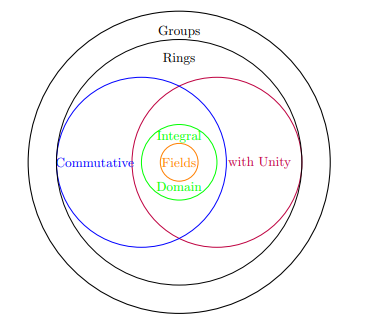
\includegraphics[width=0.5\textwidth]{Figs/algebric_structures.png}
    \caption{Algebraic Structures}
\end{figure}

\subsection{Vector Space}

A major difference between a field and a vector space is that the operations on a field \( \mathbb{F} \) are
\begin{itemize}
    \item \( +: \mathbb{F} \times \mathbb{F} \to \mathbb{F} \)
    \item \( \times: \mathbb{F} \times \mathbb{F} \to \mathbb{F} \)
\end{itemize}

but the operations on a vector space \( \mathbb{V} \) over a field \( \mathbb{F} \) are
\begin{itemize}
    \item \( +: \mathbb{V} \times \mathbb{V} \to \mathbb{V} \)
    \item \( \cdot: \mathbb{F} \times \mathbb{V} \to \mathbb{V} \)
\end{itemize}

\bigbreak

\begin{definition}{\textbf{Vector Space}} \\
    A vector space over a field \( F \) is a non-empty set \( V \) together with two operations: vector addition \( + \) and scalar multiplication \( \cdot \), satisfying the following axioms for every \( u, v, w \in V \) and \( a, b \in F \):
    \begin{enumerate}
        \item Associativity of vector addition: \( u + (v + w) = (u + v) + w \)
        \item Commutativity of vector addition: \( u + v = v + u \)
        \item Identity element of vector addition: There exists an element \( 0 \in V \), called the \textbf{zero vector}, such that \( v + 0 = v \) for all \( v \in V \).
        \item Inverse elements of vector addition: For every \( v \in V \), there exists an element \( -v \in V \), called the \textbf{additive inverse} of \( v \), such that \( v + (-v) = 0 \).
        \item Compatibility of scalar multiplication with field multiplication: \( a(bv) = (ab)v \)
        \item Identity element of scalar multiplication: \( 1v = v \), where \( 1 \) denotes the multiplicative identity in \( F \).
        \item Distributivity of scalar multiplication with respect to vector addition: \( a(u + v) = au + av \)
        \item Distributivity of scalar multiplication with respect to field addition: \( (a + b)v = av + bv \)
    \end{enumerate}
\end{definition}

\begin{example*}
Examples of vector spaces:
\begin{enumerate}
\item \( \mathbb{R}^n \) is a vector space.
\item The space \( M_{m \times n}(\mathbb{F}) \) of \( m \times n \) matrices over a field \(\mathbb{F}\) is a vector space.
\item The set of all continuous functions over some interval is a vector space.
\item The space of all differentiable functions over a certain interval is a vector space.
\end{enumerate}
\end{example*}

\begin{definition}{\textbf{Homomorphism (Vector spaces)}} \\
    Let \(V\) and \(W\) be vector spaces over the same field \(F\). A map \( T: V \to W \) is called a \textbf{homomorphism}, 
    or more specifically, a \textbf{linear transformation}, if for all vectors \(u, v \in V\) and any scalar \(c \in F\), the following conditions hold:
    \begin{itemize}
        \item \textbf{Additivity:} \( T(u + v) = T(u) + T(v) \).
        \item \textbf{Homogeneity:} \( T(c \cdot u) = c \cdot T(u) \).
    \end{itemize}
    These conditions ensure that the map \(T\) preserves the vector space structure between \(V\) and \(W\).
\end{definition}

\begin{definition}{\textbf{Image and Kernel}} \\
    Let \( V \) and \( W \) be vector spaces over a field \( F \), and let \( T: V \to W \) be a linear transformation.  \\
    The \textbf{image} of \( T \), denoted \( \text{Im}(T) \), is the set of all vectors in \( W \) that can be expressed as \( T(v) \) for some \( v \in V \). \\
    The \textbf{kernel} of \( T \), denoted \( \text{Ker}(T) \), is the set of all vectors in \( V \) that are mapped to the zero vector in \( W \), i.e., \( T(v) = 0 \).
\end{definition}


If a homomorphism is bijective, it is called an isomorphism.

\begin{definition}{\textbf{Isomorphism (Vector spaces)}} \\
    Let \( V \) and \( W \) be vector spaces over the same field \( F \). 
    A map \( T: V \to W \) is called an \textbf{isomorphism} if it is a bijective \textbf{linear transformation}, 
    meaning that \( T \) is both a homomorphism and has an inverse \( T^{-1}: W \to V \) which is also a homomorphism. 
    For \( T \) to be an isomorphism, the following conditions must be met:
    \begin{itemize}
        \item \textbf{Bijectivity:} \( T \) is one-to-one and onto.
        \item \textbf{Additivity:} \( T(u + v) = T(u) + T(v) \) for all vectors \( u, v \in V \).
        \item \textbf{Homogeneity:} \( T(c \cdot u) = c \cdot T(u) \) for all vectors \( u \in V \) and any scalar \( c \in F \).
    \end{itemize}
    An isomorphism thus establishes a perfect correspondence between the two vector spaces, preserving all vector space operations.
\end{definition}

If \(V\) and \(W\) are isomorphic, we write \(V \cong W\).


\begin{definition}{\textbf{Complex conjugate}} \\
    The complex conjugate of a complex number \( z = a + bi \) is the number \( \overline{z} = a - bi \).
\end{definition}

\begin{definition}{\textbf{The Dual Space}} \\
    Let \( V \) be a vector space over a field \( F \). The dual space of \( V \), denoted \( V^* \), is the set of all linear functionals on \( V \), 
    which are linear maps from \( V \) to \( F \). The dual space is itself a vector space over \( F \) with the operations of addition and scalar multiplication defined pointwise.
\end{definition}

\subsubsection{Basis and Dimension}

\begin{definition}{\textbf{Basis}} \\
    Let \( V \) be a vector space over a field \( F \). A set of vectors \( \{v_1, v_2, \dots, v_n\} \) in \( V \) is called a basis of \( V \) if every vector \( v \in V \) can be expressed as a unique linear combination of the basis vectors:
    \[
    v = \sum_{i=1}^n a_i v_i
    \]
    where \( a_i \in F \) are scalars. The basis vectors must be linearly independent, meaning that no vector in the set can be expressed as a linear combination of the others.
\end{definition}

\begin{definition}{\textbf{Dimension}} \\
    The dimension of a vector space \( V \) is the number of vectors in any basis of \( V \). The dimension of \( V \) is denoted \( \text{dim}(V) \).
\end{definition}

\begin{definition}{\textbf{Rank}} \\
    The rank of a matrix is the dimension of the vector space spanned by its columns.
\end{definition}

\begin{definition}{\textbf{Nullity}} \\
    The nullity of a matrix is the dimension of the vector space of solutions to the homogeneous system \( Ax = 0 \).
\end{definition}

\begin{definition}{\textbf{Rank-Nullity Theorem}} \\
    Let \( A \) be an \( m \times n \) matrix. The rank of \( A \) plus the nullity of \( A \) equals the number of columns in \( A \), i.e., 
    \[
    \text{rank}(A) + \text{nullity}(A) = n
    \]
\end{definition}

\begin{definition}{\textbf{Invertible matrix}} \\
    A square matrix \( A \) is invertible if there exists a matrix \( A^{-1} \) such that \( A A^{-1} = A^{-1} A = I \), where \( I \) is the identity matrix.
\end{definition}

\subsubsection{Cross Product and The determinant}

\begin{definition}{\textbf{Determinant}} \\
    The determinant of a square matrix \( A \) is a scalar value that is computed from the elements of \( A \) and provides significant information about the matrix.     
    For a \( 2 \times 2 \) matrix 
    \[
    det(A) = det( \begin{bmatrix} a & b \\ c & d \end{bmatrix} ) = ad - bc
    \]
    For an \( n \times n \) matrix \( A \), the determinant can be calculated using Laplace's expansion, which is defined as:
    \[
    \det(A) = \sum_{j=1}^{n} (-1)^{i+j} a_{ij} \det(A_{ij}) = \sum_{\sigma \in S_n} \text{sgn}(\sigma) \prod_{i=1}^{n} a_{i, \sigma(i)}
    \]
    where 
    \begin{itemize}
        \item \( a_{ij} \) is the element at the \( i \)-th row and \( j \)-th column of \( A \).
        \item \( A_{ij} \) is the \((n-1) \times (n-1)\) matrix obtained by removing the \( i \)-th row and \( j \)-th column from \( A \).
        \item \( S_n \) is the set of all permutations of \( n \) elements.
        \item \( \text{sgn}(\sigma) \) is the sign of the permutation \( \sigma \), which is \( +1 \) if \( \sigma \) is even and \( -1 \) if \( \sigma \) is odd.
    \end{itemize}
\end{definition}

\paragraph{Intuition for the Determinant} : \\
The determinant of a matrix can be thought of as a measure of the volume scaling factor by which a linear transformation affects a given volume when applied to a space. 
If the determinant is zero, the transformation compresses the space into a lower dimension, leading to a loss in volume. 
If the determinant is positive, the orientation of the space is preserved after transformation; if negative, the orientation is reversed.


\begin{figure}[H]
    \begin{subfigure}{0.4\textwidth}
        \centering
        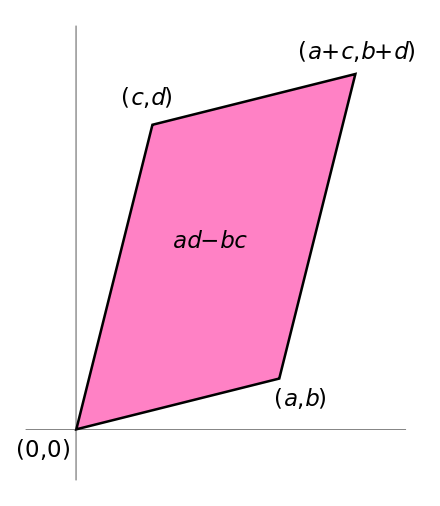
\includegraphics[width=0.8\textwidth]{Figs/area_parallellogram_as_determinant.png}
        \caption{The area of the parallelogram is the absolute value of the determinant of the matrix formed by the vectors representing the parallelogram's sides.}
    \end{subfigure}
    \hfill
    \begin{subfigure}{0.4\textwidth}
        \centering
        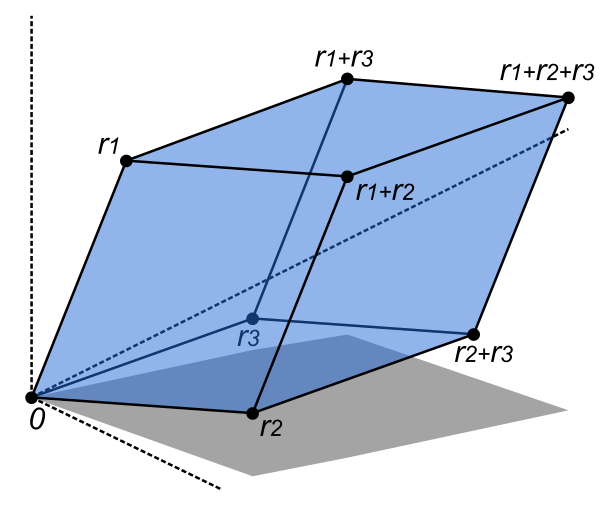
\includegraphics[width=0.8\textwidth]{Figs/determinant_parallelepiped.png}
        \caption{The volume of this parallelepiped is the absolute value of the determinant of the matrix formed by the columns constructed from the vectors r1, r2, and r3.}
    \end{subfigure}
\end{figure}

\begin{definition}{\textbf{Cross Product (in $\mathbb{R}^3$)}} \\
    The cross product of two vectors \( u = (u_1, u_2, u_3) \) and \( v = (v_1, v_2, v_3) \) in \( \mathbb{R}^3 \) is a vector \( u \times v \) defined as:
    \[
    u \times v = \begin{bmatrix} i & j & k \\ u_1 & u_2 & u_3 \\ v_1 & v_2 & v_3 \end{bmatrix} = (u_2 v_3 - u_3 v_2) i - (u_1 v_3 - u_3 v_1) j + (u_1 v_2 - u_2 v_1) k
    \]
\end{definition}

Let \( u = (x_1, y_1, z_1) \) and \( v = (x_2, y_2, z_2) \) be two vectors in \( \mathbb{R}^3 \). 
The cross product of \( u \) and \( v \) is orthogonal to both \( u \) and \( v \), and its magnitude is equal to the area of the parallelogram spanned by \( u \) and \( v \).
\begin{proof}
    We will define new axis: 
    \begin{itemize}
        \item i-axis: will be the span of \( u \)
        \item j-axis: will be orthogonal to the x-axis such that \( y \in span({u, v}) \)
        \item k-axis: will be orthogonal to the x and y axes
    \end{itemize}
    Then, we can write \( u \) and \( v \) as:
    \begin{align*}
        u &= \begin{pmatrix}x1 \\ 0 \\ 0\end{pmatrix} \quad v = \begin{pmatrix}x2 \\ y2 \\ 0\end{pmatrix} \\
        u \times v &= det\begin{pmatrix}i & j & k \\ x1 & 0 & 0 \\ x2 & y2 & 0\end{pmatrix} = 
         0 i - 0 j + x1 \cdot y2 \cdot k = \begin{pmatrix}0 \\ 0 \\ x1 \cdot y2\end{pmatrix} \\
         | \vec{w} | &= | \vec{u} | \times | \vec{v} | = | x1 \cdot y2 | = | x1 | \times | y2 | = \text{area of the parallelogram}
    \end{align*}
\end{proof}

\begin{figure}[H]
    \centering
    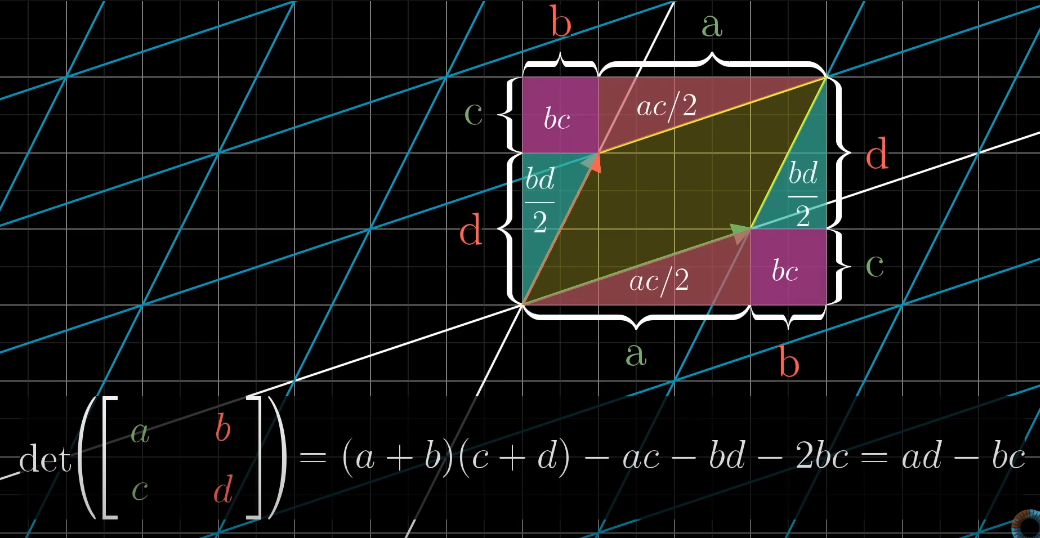
\includegraphics[width=0.7\textwidth]{Figs/determinant_in_R2.png}
    \caption{The determinant of a \( 2 \times 2 \) matrix is the area of the parallelogram spanned by the column vectors.}
\end{figure}

\begin{definition}{\textbf{Cross Product (in $\mathbb{R}^n$)}} \\
    The cross product of two vectors \( u \) and \( v \) in \( \mathbb{R}^n \) is a vector \( u \times v \) defined as:
    \[
    u \times v = \text{det} \begin{bmatrix} e_1 & e_2 & \dots & e_n \\ u_1 & u_2 & \dots & u_n \\ v_1 & v_2 & \dots & v_n \end{bmatrix}
    \]
\end{definition}

\begin{theorem}
Let \( A \) be an \( n \times n \) matrix. The following statements are equivalent:
\begin{enumerate}
    \item The matrix \( A \) is invertible.
    \item The determinant of \( A \) is nonzero (\( \det(A) \neq 0 \)).
    \item The rank of \( A \) is \( n \).
    \item \( A \) can be expressed as a product of elementary matrices.
    \item The dimension of the column space of \( A \) is \( n \).
\end{enumerate}
\end{theorem}

\begin{proof}
The equivalence of these conditions results from fundamental principles in linear algebra:
\begin{itemize}
    \item A non-zero determinant implies that the linear transformation associated with \( A \) is volume preserving and thus has no zero eigenvalues, which implies invertibility.
    \item An invertible matrix has full rank (\( n \)), meaning every row and column contributes to the matrix's span, ensuring that the transformation is onto and one-to-one.
    \item A matrix with full rank \( n \) means there are no free variables in its row-reduced form, hence it transforms \( \mathbb{R}^n \) onto itself without reducing dimension, corroborating the property of invertibility.
    \item The ability to express \( A \) as a product of elementary matrices indicates a series of elementary row operations that transform \( I \) to \( A \), again confirming the full rank and invertibility of \( A \).
\end{itemize}
\end{proof}

\todo[inline]{Add stuff about Leibniz formula for determinant}

% * * * * * * * * * * * * * * * * * * * * * * * *
% * * * * * * * * * * * * * * * * * * * * * * * *
% * * * * * * * * * * * * * * * * * * * * * * * *
% * * * * * * * * * * * * * * * * * * * * * * * *
% * * * * * * * * * * * * * * * * * * * * * * * *
% * * * * * * * * * * * * * * * * * * * * * * * *
% * * * * * * * * * * * * * * * * * * * * * * * *

\subsubsection{Eigenvalues and Eigenvectors}


\begin{definition}{\textbf{Conjugate transpose}} \\
    The conjugate transpose of a matrix \( A \) is the matrix obtained by taking the transpose of \( A \) and then taking the complex conjugate of each entry.
\end{definition}

\begin{example}
    Consider the matrix 
    \[
    A = \begin{bmatrix} 1+i & 2-i \\ 3+i & 4-2i \end{bmatrix}.
    \]
    The conjugate transpose of \( A \), denoted \( A^* \) or \( A^\dagger \), is calculated by first transposing the matrix, and then taking the complex conjugate of each element. Thus,
    \[
    A^* = \begin{bmatrix} 1-i & 3-i \\ 2+i & 4+2i \end{bmatrix}.
    \]
\end{example}

\begin{definition}{\textbf{Unitary matrix}} \\
    A square matrix \( U \) is called unitary if its conjugate transpose is equal to its inverse, i.e., \( U^* U = U U^* = I \).
\end{definition}

\begin{definition}{\textbf{Orthogonal complement}} \\
    Let \( V \) be a vector space over a field \( F \) and \( W \) be a subspace of \( V \). The orthogonal complement of \( W \), denoted \( W^\perp \), 
    is the set of all vectors in \( V \) that are orthogonal to every vector in \( W \).
\end{definition}

\begin{definition}{\textbf{Similarity}} \\
    Two matrices \( A \) and \( B \) are said to be similar if there exists an invertible matrix \( P \) such that \( B = P^{-1} A P \).
\end{definition}

\begin{definition}{\textbf{Diagonalizable}} \\
    A matrix \( A \) is said to be diagonalizable if it is similar to a diagonal matrix, i.e., 
    if there exists an invertible matrix \( P \) such that \( P^{-1} A P = D \), where \( D \) is a diagonal matrix.
\end{definition}

\begin{definition}{\textbf{Eigenvalue and Eigenvector}} \\
    Let \( A \) be an \( n \times n \) matrix. A scalar \( \lambda \) is called an eigenvalue of \( A \) if there exists a non-zero vector \( v \) such that \( A v = \lambda v \). 
    The vector \( v \) is called an eigenvector corresponding to the eigenvalue \( \lambda \).
\end{definition}

\begin{definition}{\textbf{Characteristic polynomial}} \\
    The characteristic polynomial of a square matrix \( A \) is defined as \( \text{det}(A - \lambda I) \), where \( I \) is the identity matrix.
\end{definition}

\begin{definition}{\textbf{Cayley-Hamilton Theorem}} \\
    Let \( A \) be an \( n \times n \) matrix. The Cayley-Hamilton theorem states that the matrix \( A \) satisfies its own characteristic equation, i.e., 
    \( p(A) = 0 \), where \( p(\lambda) \) is the characteristic polynomial of \( A \).
\end{definition}

\begin{definition}{\textbf{Spectral decomposition}} \\
    The spectral decomposition of a matrix \( A \) is a representation of \( A \) as a sum of its eigenvectors and eigenvalues, i.e., 
    \( A = PDP^{-1} \), where \( P \) is the matrix whose columns are the eigenvectors of \( A \) and \( D \) is the diagonal matrix of eigenvalues.
\end{definition}

\begin{definition}{\textbf{Unitary diagonalization}} \\
    A matrix \( A \) is said to be unitarily diagonalizable if it is similar to a diagonal matrix by a unitary matrix, i.e., 
    if there exists a unitary matrix \( U \) such that \( U^* A U = D \), where \( D \) is a diagonal matrix.
\end{definition}

\begin{theorem}
    Let \( A \) be an \( n \times n \) matrix. The following statements are equivalent:
    \begin{enumerate}
        \item The matrix \( A \) is unitarily diagonalizable.
        \item The matrix \( A \) is normal, i.e., \( A^* A = A A^* \).
        \item The matrix \( A \) has an orthonormal basis of eigenvectors.
    \end{enumerate}
\end{theorem} 

% * * * * * * * * * * * * * * * * * * * * * * * *
% * * * * * * * * * * * * * * * * * * * * * * * *
% * * * * * * * * * * * * * * * * * * * * * * * *
% * * * * * * * * * * * * * * * * * * * * * * * *
% * * * * * * * * * * * * * * * * * * * * * * * *
% * * * * * * * * * * * * * * * * * * * * * * * *
% * * * * * * * * * * * * * * * * * * * * * * * *


\subsubsection{Quadradic and Bilinear Forms}

\begin{definition}{\textbf{Congruence}} \\
    Two matrices \( A \) and \( B \) are said to be congruent if there exists an invertible matrix \( P \) such that \( B = P^T A P \).
\end{definition}


\begin{definition}{\textbf{Quadratic Form}} \\
    A quadratic form on a vector space \( V \) over a field \( F \) is a function \( Q: V \to F \) that is homogeneous of degree 2, 
    meaning that for all \( v \in V \) and \( a \in F \), the quadratic form satisfies:
    \begin{enumerate}
        \item Homogeneity: \( Q(av) = a^2 Q(v) \)
        \item Additivity: \( Q(u + v) = Q(u) + Q(v) \)
    \end{enumerate}
\end{definition}

Any $n \times n$ matrix $A$ defines a quadratic form $Q(v) = v^T A v$ for $v \in \mathbb{R}^n$.  \\
Two matrices $A$ and $B$ define the same quadratic form if and only if they have the same elements on the diagonal and $a_{ij} + a_{ji} = b_{ij} + b_{ji}$ for all $i \neq j$. \\
In general a quadratic form can be written as $Q(v) = v^T A v$ where $A$ is a symmetric matrix. \\
The correspondence between quadratic forms and symmetric matrices is one-to-one, when the basis is fixed.

\begin{definition}{\textbf{Bilinear Form}}
    A bilinear form on a vector space \( V \) over a field \( F \) is a function \( B: V \times V \to F \) that is linear in each of its two arguments independently. This means that for all \( u, v, w \in V \) and \( a \in F \), the bilinear form satisfies:
    \begin{enumerate}
        \item Linearity in the first argument: \( B(au + w, v) = a B(u, v) + B(w, v) \)
        \item Linearity in the second argument: \( B(u, av + w) = a B(u, v) + B(u, w) \)
    \end{enumerate}
    The bilinear form \( B \) is symmetric if \( B(u, v) = B(v, u) \) for all \( u, v \in V \).
\end{definition}

\paragraph{Matrix Representation of a Bilinear Form}: \\ 
Every bilinear form \( B \) on a finite-dimensional vector space \( V \) can be represented by a matrix \( A \) with respect to a basis 
\( \{e_1, e_2, \dots, e_n\} \) of \( V \). 
The entry \( a_{ij} \) in the matrix is defined as \( a_{ij} = B(e_i, e_j) \). Thus, the matrix \( A \) of the bilinear form \( B \) is given by:
\[
A = [a_{ij}] \quad \text{where} \quad a_{ij} = B(e_i, e_j)
\]
Let \( u = \sum_{i=1}^n u_i e_i \) and \( v = \sum_{j=1}^n v_j e_j \) be vectors in \( V \). The matrix representation of the bilinear form \( B \) is then:
\[
B(u, v) = u^T A v 
= \begin{bmatrix} u_1 & u_2 & \cdots & u_n \end{bmatrix} \begin{bmatrix} a_{11} & a_{12} & \cdots & a_{1n} \\ a_{21} & a_{22} & \cdots & a_{2n} \\ \vdots & \vdots & \ddots & \vdots \\ a_{n1} & a_{n2} & \cdots & a_{nn} \end{bmatrix} \begin{bmatrix} v_1 \\ v_2 \\ \vdots \\ v_n \end{bmatrix}
= \sum_{i=1}^n \sum_{j=1}^n a_{ij} u_i v_j
\]


\begin{theorem}{:} \\
    Two matrices \( A \) and \( B \) are congruent if and only if they represent the same quadratic (bilinear) form, i.e., \( Q_A(v) = Q_B(v) \) for all \( v \).
\end{theorem}

\begin{proof} 
    Let $v_1, v_2, \ldots, v_n$ be some basis in $\mathbb{R}^n$, and consider the matrix $P$ whose columns are these basis vectors. 
    Then $P$ is non singular and $\forall x \in \mathbb{R}^n$, $\exists y \in \mathbb{R}^n$ such that $x = Py$. \\
    \\
    Let \( A \) and \( B \) be congruent matrices, i.e., \( B = P^T A P \) for some invertible matrix \( P \). 
    Then, for any vector \( v \), we have:
    \[
    Q_B(v) = v^T B v = v^T P^T A P v = (Pv)^T A (Pv) 
    \]
    Thus, the quadratic form \( Q_B(v) \) is represented by the matrix \( A \) in the basis \( Pv \). 
\end{proof}


\paragraph{Differences Between Congruence and Similarity}: \\

While both congruence and similarity involve transformations of matrices via invertible matrices, they are used in different contexts and have distinct algebraic implications:

\begin{itemize}
    \item \textbf{Congruence}: This relationship focuses on the geometric properties of matrices, 
    particularly those representing quadratic forms or symmetric bilinear forms. When two matrices \( A \) and \( B \) are congruent, 
    it implies that they represent the same quadratic form but in possibly different coordinate systems. 
    The transformation \( B = P^T A P \) can be interpreted as a change of basis in which the basis vectors are orthogonalized or rotated, 
    maintaining the essence of the geometric structure represented by the matrix. 
    Thus, congruence preserves the type of conic sections (e.g., ellipses, hyperbolas) or other geometric objects described by these forms under orthogonal transformations.

    \item \textbf{Similarity}: Similarity transformations are concerned with the preservation of eigenvalues of a matrix. 
    When \( A \) and \( B \) are similar, they represent the same linear transformation expressed in different bases. 
    The condition \( B = P^{-1} A P \) indicates that changing the basis does not alter the intrinsic properties of the linear transformation such as 
    trace, determinant, and eigenvalues. Essentially, similarity is related to the fundamental operations of the matrix and does not 
    concern itself directly with geometric interpretations in the same way as congruence. 

\end{itemize}

% * * * * * * * * * * * * * * * * * * * * * * * *
% * * * * * * * * * * * * * * * * * * * * * * * *
% * * * * * * * * * * * * * * * * * * * * * * * *
% * * * * * * * * * * * * * * * * * * * * * * * *
% * * * * * * * * * * * * * * * * * * * * * * * *
% * * * * * * * * * * * * * * * * * * * * * * * *
% * * * * * * * * * * * * * * * * * * * * * * * *

\subsubsection{Inner Product Space}

\begin{definition}{\textbf{Inner Product Space}} \\
    An inner product space is a vector space \( V \) over a field \( F \) equipped with an inner product, which is a function that associates each pair of vectors \( u, v \) in \( V \) with a scalar in \( F \), denoted \( \langle u, v \rangle \), and satisfies the following properties for all \( u, v, w \in V \) and \( a \in F \):
    \begin{enumerate}
        \item Linearity in the first argument: \( \langle au + v, w \rangle = a \langle u, w \rangle + \langle v, w \rangle \)
        \item Conjugate symmetry: \( \langle u, v \rangle = \overline{\langle v, u \rangle} \)
        \item Positive-definiteness: \( \langle u, u \rangle \geq 0 \) and \( \langle u, u \rangle = 0 \) if and only if \( u = 0 \)
    \end{enumerate}
\end{definition}


\begin{theorem}{\textbf{Inner product and PD matrix}} \\
    Let \( V \) be an inner product space over a field \( F \). The inner product \( \langle u, v \rangle \) is positive-definite if and only if 
    the matrix representing the inner product in any basis is symmetric positive-definite (SPD).
\end{theorem}

\begin{theorem}{A matrix \( A \) defines inner product $\iff$ congruent to identity matrix} \\
\end{theorem}

\begin{proof}
    The proof involves showing that the matrix \( A \) is congruent to \( I \) if and only if it defines an inner product. \\
    \\
    \textbf{If \( A \) defines an inner product, then \( A \) is congruent to \( I \)}: \\
    Assume that the matrix \( A \) on a vector space \( V \) of dimension \( n \) defines an inner product. By definition, this inner product, denoted as \( \langle \mathbf{u}, \mathbf{v} \rangle \), for any vectors \( \mathbf{u}, \mathbf{v} \in V \) can be expressed in terms of the matrix \( A \) as:
    \[
    \langle \mathbf{u}, \mathbf{v} \rangle = \mathbf{u}^T A \mathbf{v}.
    \]

    To show that \( A \) is congruent to \( I \), we need to find an invertible matrix \( P \) such that:
    \[
    P^T A P = I.
    \]

    Since \( A \) defines an inner product, it must be symmetric and positive definite. A symmetric matrix \( A \) can be orthogonally diagonalized to a diagonal matrix \( D \) with positive diagonal entries because it is positive definite. This orthogonal diagonalization can be represented as:
    \[
    A = Q^T D Q,
    \]
    where \( Q \) is an orthogonal matrix (i.e., \( Q^{-1} = Q^T \)) and \( D \) is a diagonal matrix with positive entries along the diagonal.

    The matrix \( D \) can be transformed into the identity matrix by scaling. Let \( D^{1/2} \) be the diagonal matrix whose diagonal entries are the square roots of the corresponding diagonal entries of \( D \). Define a new matrix \( P \) as:
    \[
    P = Q D^{-1/2}.
    \]

    Then,
    \[
    P^T A P = (Q D^{-1/2})^T (Q^T D Q) (Q D^{-1/2}) = D^{-1/2} Q^T Q^T D Q Q D^{-1/2} = D^{-1/2} D D^{-1/2} = I.
    \]

    \medbreak
    \textbf{If \( A \) is congruent to \( I \), then \( A \) defines an inner product}: \\
    Suppose that the matrix \( A \) is congruent to the identity matrix \( I \). Then, there exists an invertible matrix \( P \) such that \( A = P^T I P = P^T P \). 
    Since \( P \) is invertible, the matrix \( P^T P \) is symmetric positive-definite, and hence defines an inner product. 
    Therefore, the matrix \( A \) defines an inner product. \\

\end{proof}

\begin{definition}{\textbf{Norm}} \\
    The norm of a vector \( v \) in an inner product space is defined as \( ||v|| = \sqrt{\langle v, v \rangle} \).
\end{definition}


\begin{definition}{\textbf{Hermetian adjoint}} \\
    Let \( V \) be an inner product space over a field \( F \). 
    The Hermetian adjoint of a linear operator \( T: V \to V \) is the unique linear operator \( T^*: V \to V \) such that for all \( u, v \in V \), we have \( \langle Tu, v \rangle = \langle u, T^*v \rangle \).
\end{definition}

A classic exmaple of an inner product space is the \textbf{Euclidean space} \( \mathbb{E}^n \), which is a vector space equipped with 
the inner product \( \langle u, v \rangle = u^T v \).
The geometry of Euclidean space follows the familiar rules of Euclidean geometry, which include notions such as angles, lengths, and the Pythagorean theorem.
It is always complete, meaning that every Cauchy sequence in Euclidean space converges to a point within the space.
Euclidean space can be thought of as the "standard" \( n \)-dimensional space that conforms to our intuitive geometric concepts.



% * * * * * * * * * * * * * * * * * * * * * * * * 
% * * * * * * * * * * * * * * * * * * * * * * * * 
% * * * * * * * * * * * * * * * * * * * * * * * * 
% * * * * * * * * * * * * * * * * * * * * * * * * 
% * * * * * * * * * * * * * * * * * * * * * * * * 
% * * * * * * * * * * * * * * * * * * * * * * * * 
% * * * * * * * * * * * * * * * * * * * * * * * * 
% * * * * * * * * * * * * * * * * * * * * * * * * 
% * * * * * * * * * * * * * * * * * * * * * * * * 
% * * * * * * * * * * * * * * * * * * * * * * * * 
% * * * * * * * * * * * * * * * * * * * * * * * * 
% * * * * * * * * * * * * * * * * * * * * * * * * 
% * * * * * * * * * * * * * * * * * * * * * * * * 
% * * * * * * * * * * * * * * * * * * * * * * * * 
% * * * * * * * * * * * * * * * * * * * * * * * * 
% * * * * * * * * * * * * * * * * * * * * * * * * 
% * * * * * * * * * * * * * * * * * * * * * * * * 
% * * * * * * * * * * * * * * * * * * * * * * * * 
% * * * * * * * * * * * * * * * * * * * * * * * * 

\chapter{Multivariable Calculus}

\begin{definition}{Diffrentiability, single variable} \\
Let $f: (a,b) \rightarrow \mathbb{R}$ be a function. We say that $f$ is differentiable at $x_0 \in (a,b)$ if
\begin{equation}
    \lim_{h \rightarrow 0} \frac{f(x_0 + h) - f(x_0)}{h}
\end{equation}
exists. If $f$ is differentiable at $x_0$, then $f'(x_0)$ is the derivative of $f$ at $x_0$.
\end{definition} 

\bigbreak

\begin{definition}{Diffrentiability, single variable (alternative)} \\
Let $f: (a,b) \rightarrow \mathbb{R}$ be a function. We say that $f$ is differentiable at $x_0 \in (a,b)$ if there exists a number m such that:
\begin{equation}
    f(x_0 + h) = f(x_0) + m \cdot h + E(h) \text{ where } \lim_{h \rightarrow 0} \frac{E(h)}{h} = 0
\end{equation}
If $f$ is differentiable at $x_0$, then $f'(x_0) = m$ is the derivative of $f$ at $x_0$.
\end{definition}

\bigbreak

Suppose the $S \subseteq \mathbb{R}^n$ and $f: S \rightarrow \mathbb{R}$ is a function. 

\bigbreak

\begin{definition}{Limit, multivariate function} \\
We say that the limit of $f$ at $x_0$ is $L$ if for all $\epsilon > 0$, there exists $\delta > 0$ such that 
for all $x$ such that $||x - x_0|| < \delta$, we have $|f(x) - L| < \epsilon$.
\end{definition}

\begin{definition}{Diffrentiability, multivariable} \\
    Let $f: \mathbb{R}^n \rightarrow \mathbb{R}$ be a function. We say that $f$ is differentiable at $x_0$ if there exists a vector m $\in \mathbb{R}^n$ such that:
    \begin{equation}
        \lim_{h \rightarrow 0} \frac{f(x_0 + h) - f(x_0) - m \cdot h}{||h||} = 0
    \end{equation}
    If $f$ is differentiable at $x_0$, then $m$ is the gradient of $f$ at $x_0$, denoted $\nabla f(x_0)$.
\end{definition}
    
\bigbreak

\begin{definition}{Diffrentiability, multivariable (alternative)} \\
We say that $f$ is differentiable at $x_0$ if there exists a vector m $\in \mathbb{R}^n$ such that:
\begin{equation}
    f(x_0 + h) = f(x_0) + m^T \cdot h + E(h) \text{ where } \lim_{h \rightarrow 0} \frac{E(h)}{||h||} = 0
\end{equation}
If $f$ is differentiable at $x_0$, then $m$ is the gradient of $f$ at $x_0$, denoted $\nabla f(x_0)$.
\end{definition}

\bigbreak

\begin{definition}{\textbf{Differentiability of a function $f: \mathbb{R}^n \rightarrow \mathbb{R}^m$}} \\
    Let $f: \mathbb{R}^n \rightarrow \mathbb{R}^m$ be a function. We say that $f$ is differentiable at $x_0$ 
    if there exists a matrix $A \in \mathbb{R}^{m \times n}$ such that:
    \begin{equation}
        \lim_{h \rightarrow 0} \frac{||f(x_0 + h) - f(x_0) - A \cdot h||}{||h||} = 0
    \end{equation}
    If $f$ is differentiable at $x_0$, then $A$ is the Jacobian matrix of $f$ at $x_0$, denoted $J_f(x_0)$.
\end{definition}


\begin{definition}{The Jacobian matrix} \\
    The Jacobian matrix of $f: \mathbb{R}^n \rightarrow \mathbb{R}^m$ at $x$ is the matrix of partial derivatives of $f$ at $x$:
    \[
        J = \left[
        \begin{array}{ccc}
        \frac{\partial f}{\partial x_1} & \cdots & \frac{\partial f}{\partial x_n}
        \end{array}
        \right]
        = \left[
        \begin{array}{c}
        \nabla^T f_1 \\
        \vdots \\
        \nabla^T f_m
        \end{array}
        \right]
        = \left[
        \begin{array}{ccc}
        \frac{\partial f_1}{\partial x_1} & \cdots & \frac{\partial f_1}{\partial x_n} \\
        \vdots & \ddots & \vdots \\
        \frac{\partial f_m}{\partial x_1} & \cdots & \frac{\partial f_m}{\partial x_n}
        \end{array}
        \right]
    \]
    \end{definition}
    
    \begin{example*}
    Let $f: \mathbb{R}^2 \rightarrow \mathbb{R}^2$ be a function defined by $f(x,y) = (x^2, y^2)$. Then the Jacobian matrix of $f$ is:
    \begin{equation}
        J_f(x,y) = \begin{bmatrix}
        2x & 0 \\
        0 & 2y
        \end{bmatrix}
    \end{equation}
\end{example*}
    

\begin{definition}{Partial Derivative} \\
The partial derivative of $f$ with respect to the $i$-th variable at $x$ is:
\begin{equation}
    \frac{\partial f}{\partial x_i}(x) = \lim_{h \rightarrow 0} \frac{f(x + h \cdot e_i) - f(x)}{h}
\end{equation}
where $e_i$ is the $i$-th standard basis vector.
\end{definition}

\bigbreak

\begin{theorem}(Diffrentiability vs. Partial Derivatives) \\
If $f$ is differentiable at $x$, then all partial derivatives of $f$ exist at $x$ and:
\begin{equation}
    \nabla f(x) = \left( \frac{\partial f}{\partial x_1}(x), \ldots, \frac{\partial f}{\partial x_n}(x) \right)
\end{equation}    
\end{theorem}

\bigbreak

\begin{itemize}
    \item If any partial derivative of $f$ does not exist at $x$, then $f$ is not differentiable at $x$.
    \item If all partial derivatives of $f$ exist at $x$, then $f$ may still not be differentiable at $x$ 
    and the vector $m = \nabla f(x)$ is the only possible vector that satisfies the definition of differentiability.
\end{itemize}

\bigbreak

\begin{definition}
    The partial derivative of the function \( f_i \) with respect to the variable \( x_j \), denoted by \( \frac{\partial f_i}{\partial x_j} \), is defined as the limit
    \[
    \frac{\partial f_i}{\partial x_j} = \lim_{h \to 0} \frac{f_i(x_1, \ldots, x_j + h, \ldots, x_n) - f_i(x_1, \ldots, x_j, \ldots, x_n)}{h}
    \]
\end{definition}

\begin{definition}{Continuously Differentiable} \\
We say that $f$ is continuously differentiable or of class $C^1$  if all partial derivatives of $f$ exist and are continuous at every point in $S$.
\end{definition}

\bigbreak

\begin{theorem}
If $f$ is continuously differentiable, then $f$ is differentiable.
\end{theorem}

\bigbreak

\begin{definition}{The directional derivative} \\
For a given $x \in S$ and a unit vector $u \in \mathbb{R}^n$, the directional derivative of $f$ at $x$ in the direction of $u$ is:
\begin{equation}
    \partial_u f(x) = \lim_{h \rightarrow 0} \frac{f(x + h \cdot u) - f(x)}{h}
\end{equation}
Equivalently, $\partial_u f(x) = g'(0)$ where $g(h) = f(x + h \cdot u)$.
\end{definition}

\bigbreak

\begin{theorem}
If $f$ is differentiable at $x$, then for all $u \in \mathbb{R}^n$, the directional derivative of $f$ at $x$ in the direction of $u$ exists and is given by:
\begin{equation}
    \partial_u f(x) = \nabla f(x) \cdot u
\end{equation}
\end{theorem}

\bigbreak

\begin{theorem}{Fermat's Theorem} \\
If $f$ is differentiable at $x$ and $x$ is a local minimum of $f$, then $\nabla f(x) = 0$.
\end{theorem}

\bigbreak

\begin{definition}{\textbf{Differential of a function at a point} (in $\mathbb{R}^n$)} \\
    Let \( f: \mathbb{R}^n \to \mathbb{R} \) be a function of class \( C^1 \). \\
    The differential of f at a point \( p \in \mathbb{R}^n \) is the linear map \( df_p : \mathbb{R}^n \to \mathbb{R} \) defined as
    \begin{equation*}
        df_p(v) = \sum_{i=1}^{n} \frac{\partial f}{\partial x_i}(p) \cdot v_i
    \end{equation*}
    for every \( v = (v_1, \ldots, v_n) \in \mathbb{R}^n \).
\end{definition}

\bigbreak

The relation between the differential and the gradient: \\  
\begin{equation}
    df_p(v) = \nabla f(p) \cdot v
\end{equation}

Recall that the gradient is the Jacobian matrix of the function \( f: \mathbb{R}^n \to \mathbb{R} \), 
So in general the relation between the differential and the Jacobian matrix is:
\begin{equation}
    df_p(v) = J_f(p) \cdot v
\end{equation}

The range of the differential is the set of all linear functions of the form \( df_p(v) = J_f(p) \cdot v \) for \( v \in \mathbb{R}^n \),
and is called the tangent space to the point \( p \) of the graph of the function \( f \).

\bigbreak

\begin{theorem}
Suppose that $f: S \rightarrow \mathbb{R}$ is differentiable at $x$. Then $\nabla f(x)$ is orthogonal to the level set of $f$ that passes through $x$.    
\end{theorem}

\bigbreak

\begin{theorem}{The mean value theorem} \\
If $f: S \rightarrow \mathbb{R}$ is differentiable on the open interval between $a$ and $b$, then there exists $c \in [a,b]$ such that:
\begin{equation}
    f(b) - f(a) = \nabla f(c) \cdot (b-a)
\end{equation}
where $[a,b] = {a + t(b-a) | t \in [0,1]}$.
\end{theorem}

\bigbreak

\begin{definition}{Second-order partial derivatives} \\
Suppose that f is a $C^1$ function. If the partial derivatives of f are differentiable, then the second-order partial derivatives of f are:
\begin{equation}
    \frac{\partial^2 f}{\partial x_i \partial x_j} = \frac{\partial}{\partial x_i} \left( \frac{\partial f}{\partial x_j} \right) 
\end{equation}
Equivalently, $\frac{\partial^2 f}{\partial i \partial j} = \partial_j \partial_j f$.
If i = j we denote $\frac{\partial^2 f}{\partial x_i^2}$ or $(\partial_i^2 f$
\end{definition}

\bigbreak

\begin{definition}\label{def:C^2_class}{The $C^2$ class} \\
We say that $f$ is of class $C^2$ if all second-order partial derivatives of $f$ exist and are continuous.
\end{definition}

\bigbreak

\begin{theorem}{Clairaut's Theorem} \\
If $f$ is of class $C^2$, then $\frac{\partial^2 f}{\partial x_i \partial x_j} = \frac{\partial^2 f}{\partial x_j \partial x_i}$.
\end{theorem}

\bigbreak

\begin{definition}{Hessian Matrix} \\
The Hessian matrix of $f$ at $x$ is the matrix of second-order partial derivatives of $f$ at $x$:
\begin{equation}
    \nabla^2 f(x) = \begin{bmatrix}
    \frac{\partial^2 f}{\partial x_1^2} & \frac{\partial^2 f}{\partial x_1 \partial x_2} & \ldots & \frac{\partial^2 f}{\partial x_1 \partial x_n} \\
    \frac{\partial^2 f}{\partial x_2 \partial x_1} & \frac{\partial^2 f}{\partial x_2^2} & \ldots & \frac{\partial^2 f}{\partial x_2 \partial x_n} \\
    \vdots & \vdots & \ddots & \vdots \\
    \frac{\partial^2 f}{\partial x_n \partial x_1} & \frac{\partial^2 f}{\partial x_n \partial x_2} & \ldots & \frac{\partial^2 f}{\partial x_n^2}
    \end{bmatrix}
\end{equation}
\end{definition}

\bigbreak

\begin{corollary*}{The interpretation of the Hessian matrix} \\
Let $u \in \mathbb{R}^n$ be a unit vector. then
\begin{equation}
    \partial_{uu}^2 f(x) = \sum_{i,j=1}^n \partial_{ij} f(x) u_i u_j  = u^T \nabla^2 f(x) u
\end{equation}
\end{corollary*}

\bigbreak

We can generalize the Hessian matrix to functions $f: \mathbb{R}^n \rightarrow \mathbb{R}^m$ by defining the Hessian tensor.
\begin{definition}{\textbf{Hessian Tensor}} \\
    The Hessian tensor of $f: \mathbb{R}^n \rightarrow \mathbb{R}^m$ at $x$ is the tensor of second-order partial derivatives of $f$ at $x$:
    \begin{equation}
        \mathbf{H}(x) = \begin{bmatrix}
        \nabla^2 f_1(x), &\nabla^2 f_2(x), &\ldots, &\nabla^2 f_m(x)
        \end{bmatrix}
    \end{equation}
    where $\nabla^2 f_i(x)$ is the Hessian matrix of $f_i$ at $x$.
\end{definition}

% * * * * * * * * * * * * * * * * * * * * * * * *
% * * * * * * * * * * * * * * * * * * * * * * * *
% * * * * * * * * * * * * * * * * * * * * * * * *
% * * * * * * * * * * * * * * * * * * * * * * * *
% * * * * * * * * * * * * * * * * * * * * * * * *
% * * * * * * * * * * * * * * * * * * * * * * * *
% * * * * * * * * * * * * * * * * * * * * * * * *

\section{Curves}

\begin{definition}{\textbf{Curve in \( \mathbb{R}^n \)}} \\
    A curve in \( \mathbb{R}^n \) is a function \( \gamma: I \to \mathbb{R}^n \), where \( I \) is an interval in \( \mathbb{R} \).
    In other words, a curve \( \gamma(t) = (\gamma_1(t), \gamma_2(t), \ldots, \gamma_n(t)) \) is a parametric representation of a path in \( \mathbb{R}^n \).
\end{definition}

\begin{definition}{\textbf{Differentiable curve in \( \mathbb{R}^n \)}} \\ 

    A differentiable curve in \( \mathbb{R}^n \) is a function \( \gamma: I \to \mathbb{R}^n \), where \( I \) is an interval in \( \mathbb{R} \), 
    such that each of the component functions of \( \gamma \) is differentiable at every point in \( I \). 

    In other words, a curve \( \gamma(t) = (\gamma_1(t), \gamma_2(t), \ldots, \gamma_n(t)) \) is differentiable 
    if each \( \gamma_i(t) \) has a derivative \( \gamma_i'(t) \) for all \( t \in I \).

    Formally, a curve \( \gamma: (a, b) \to \mathbb{R}^n \) is differentiable at a point \( t_0 \in (a, b) \) if the limit
    \[
    \lim_{t \to t_0} \frac{\gamma(t) - \gamma(t_0)}{t - t_0}
    \]
    exists, and is a vector in \( \mathbb{R}^n \). 
\end{definition}

This vector is the tangent vector to the curve at the point \( \gamma(t_0) \), and the collection of all such tangent vectors as
\( t \) varies in \( (a, b) \) forms a vector field along the curve, provided the curve is differentiable on the interval.


\begin{example}{\textbf{The Unit Circle in \( \mathbb{R}^2 \) as a curve}} \\
    Consider the curve \( \gamma: [0, 2\pi] \to \mathbb{R}^2 \) defined by
    \[
    \gamma(t) = (\cos(t), \sin(t)) 
    \]
    This curve traces out the unit circle in \( \mathbb{R}^2 \) as \( t \) varies from 0 to \( 2\pi \).

    The derivative of the curve \( \gamma \) at any point \( t \) is given by:
    \[
    \gamma'(t) = \left( -\sin(t), \cos(t) \right) = \left( \cos\left(t + \frac{\pi}{2}\right), \sin\left(t + \frac{\pi}{2}\right) \right)
    \]
    This derivative represents the tangent vector to the curve at each point, 
    showing the direction of motion along the circle. The magnitude of this tangent vector is always 1, indicating constant speed along the curve.
\end{example}

Note:  
\begin{itemize}
    \item The derivative of the curve \( \gamma : [a,b] \to \mathbb{R}^n \) is a vector in \( \mathbb{R}^n \). 
    \item In general, the derivative of a curve in \( \mathbb{R}^n \) is orthogonal to the curve itself at every point.
\end{itemize}


\begin{figure}[H]
    \centering
    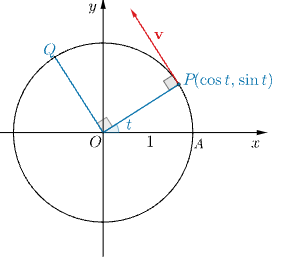
\includegraphics[width=0.3\textwidth]{./figs/unit_circle_curve_R2.png}
    \caption{The curve \( \gamma(t) = (\cos(t), \sin(t)) \) traces out the unit circle.}
\end{figure}

\begin{definition}{Approximation of a curve by linear segments} \\
    A curve in \( \mathbb{R}^n \) can be approximated by a sequence of linear segments connecting points along the curve.
    This process is called rectification of a curve, and the resulting sequence of line segments is called the rectification of the curve.
\end{definition}

\begin{figure}[H]
    \centering
    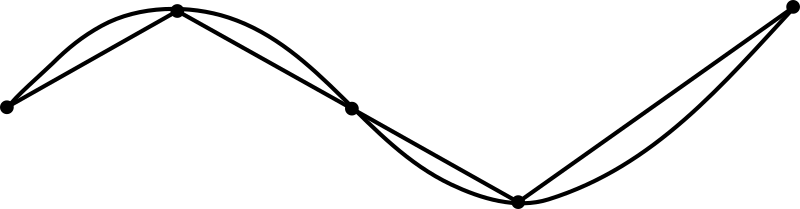
\includegraphics[width=0.3\textwidth]{./figs/Arclength.png}
    \caption{Rectification of a curve.}
\end{figure}

If the curve is differentiable, the rectification of the curve is a piecewise linear approximation of the curve that converges 
to the curve as the length of the segments approaches zero. 
As the length of the segments approaches zero, the rectification of the curve at each point converges to the tangent vector to the curve at that point.

\begin{definition}{\textbf{Arc length of a curve}} \\
    The arc length of a curve \( \gamma: [a, b] \to \mathbb{R}^n \) is the integral of the magnitude of the derivative of the curve over the interval:
    \[
    L = \int_{a}^{b} ||\gamma'(t)|| \, dt
    \]
    This integral represents the total distance traveled along the curve from \( \gamma(a) \) to \( \gamma(b) \).
\end{definition}


\todo [inline]{Add the definition of curvature of a curve with history of a circle.}
\begin{definition}{\textbf{Curvature of a curve}} \\
    The curvature of a curve \( \gamma: [a, b] \to \mathbb{R}^n \) is a measure of how much the curve deviates from a straight line at each point.
    The curvature is defined as the magnitude of the derivative of the tangent vector to the curve with respect to arc length:
    \[
    \kappa = \left|\frac{d\mathbf{T}}{ds}\right|
    \]
    where \( \mathbf{T} \) is the unit tangent vector to the curve, and \( s \) is the arc length parameter.
\end{definition}






% * * * * * * * * * * * * * * * * * * * * * * * *
% * * * * * * * * * * * * * * * * * * * * * * * *
% * * * * * * * * * * * * * * * * * * * * * * * *
% * * * * * * * * * * * * * * * * * * * * * * * *
% * * * * * * * * * * * * * * * * * * * * * * * *
% * * * * * * * * * * * * * * * * * * * * * * * *
% * * * * * * * * * * * * * * * * * * * * * * * *

\section{Taylor series}
\begin{definition}{Taylor Series} \\
Let $f: \mathbb{R} \rightarrow \mathbb{R}$ be a function that is $k$ times differentiable at $x_0$. Then the Taylor series of $f$ at $x_0$ is given by:
\begin{equation}
    f(x) = f(x_0) + f'(x_0)(x-x_0) + \frac{f''(x_0)}{2!}(x-x_0)^2 + \ldots + \frac{f^{(k)}(x_0)}{k!}(x-x_0)^k + R_k(x)
\end{equation}
where $R_k(x) = \frac{f^{(k+1)}(c)}{(k+1)!}(x-x_0)^{k+1}$ for some $c$ between $x$ and $x_0$.
\end{definition}

\bigbreak

\begin{definition}{Taylor Series for Multivariable Functions (k=2) } \\
Let $f: \mathbb{R}^n \rightarrow \mathbb{R}$ be a function that is $C^2$ at $x_0$. Then for any h such that $x_0 + h \in S$, there exists $\theta \in [0,1]$ such that:
\begin{equation}
    f(x_0 + h) = f(x_0) + \nabla f(x_0) \cdot h + \frac{1}{2} h^T \nabla^2 f(x_0 + \theta h) h
\end{equation}
\end{definition}

% * * * * * * * * * * * * * * * * * * * * * * * * 
% * * * * * * * * * * * * * * * * * * * * * * * * 
% * * * * * * * * * * * * * * * * * * * * * * * * 
% * * * * * * * * * * * * * * * * * * * * * * * * 
% * * * * * * * * * * * * * * * * * * * * * * * * 
% * * * * * * * * * * * * * * * * * * * * * * * * 
% * * * * * * * * * * * * * * * * * * * * * * * * 
% * * * * * * * * * * * * * * * * * * * * * * * * 
% * * * * * * * * * * * * * * * * * * * * * * * * 
% * * * * * * * * * * * * * * * * * * * * * * * * 
% * * * * * * * * * * * * * * * * * * * * * * * * 
% * * * * * * * * * * * * * * * * * * * * * * * * 
% * * * * * * * * * * * * * * * * * * * * * * * * 
% * * * * * * * * * * * * * * * * * * * * * * * * 
% * * * * * * * * * * * * * * * * * * * * * * * * 
% * * * * * * * * * * * * * * * * * * * * * * * * 
% * * * * * * * * * * * * * * * * * * * * * * * * 
% * * * * * * * * * * * * * * * * * * * * * * * * 
% * * * * * * * * * * * * * * * * * * * * * * * * 


\chapter{Convexity and Optimization}

\section{Important subsets of $\mathbb{R}^n$}

\begin{definition}{Open set} \\
A set $S \subseteq \mathbb{R}^n$ is open if for all $x \in S$, there exists $\epsilon > 0$ such that $B(x, \epsilon) \subseteq S$.
\end{definition}

\begin{definition}{Closed set} \\
A set $S \subseteq \mathbb{R}^n$ is closed if its complement is open.
\end{definition}

\begin{definition}{Interior point} \\
A point $x \in S$ is an interior point of $S$ if there exists $\epsilon > 0$ such that $B(x, \epsilon) \subseteq S$.
\end{definition}

\begin{corollary}{Open set characterization} \\
A set $S \subseteq \mathbb{R}^n$ is open if and only if every point in $S$ is an interior point of $S$.
\end{corollary}

\begin{definition}{Boundary point} \\
A point $x \in S$ is a boundary point of $S$ if for all $\epsilon > 0$, $B(x, \epsilon) \cap S \neq \emptyset$ and $B(x, \epsilon) \cap S^c \neq \emptyset$.
\end{definition}

\begin{definition}{Half-space} \\
A half-space in $\mathbb{R}^n$ is a set of the form $\{x \in \mathbb{R}^n : a^T x \leq b\}$ for some $a \in \mathbb{R}^n$ and $b \in \mathbb{R}$.
\end{definition}

\begin{definition}{Hyperplane} \\
A hyperplane in $\mathbb{R}^n$ is a set of the form $\{x \in \mathbb{R}^n : a^T x = b\}$ for some $a \in \mathbb{R}^n$ and $b \in \mathbb{R}$.
\end{definition}

\begin{definition}{Polyhedron (Polyhedra)} \\
A polyhedron in $\mathbb{R}^n$ is a set of the form $\{x \in \mathbb{R}^n : Ax \leq b\}$ for some $A \in \mathbb{R}^{m \times n}$ and $b \in \mathbb{R}^m$.
Equivalently, a polyhedron is the intersection of finitely many half-spaces.
\end{definition}

\begin{definition}{Polytope} \\
A polytope in $\mathbb{R}^n$ is a bounded polyhedron - i.e., there exists $r > 0$ such that $\forall x \in \{x \in \mathbb{R}^n : Ax \leq b\} \implies ||x|| \leq r$.
Equivalently, a polytope is the convex hull of finitely many points.
\end{definition}

\begin{figure}[H]
    \centering
    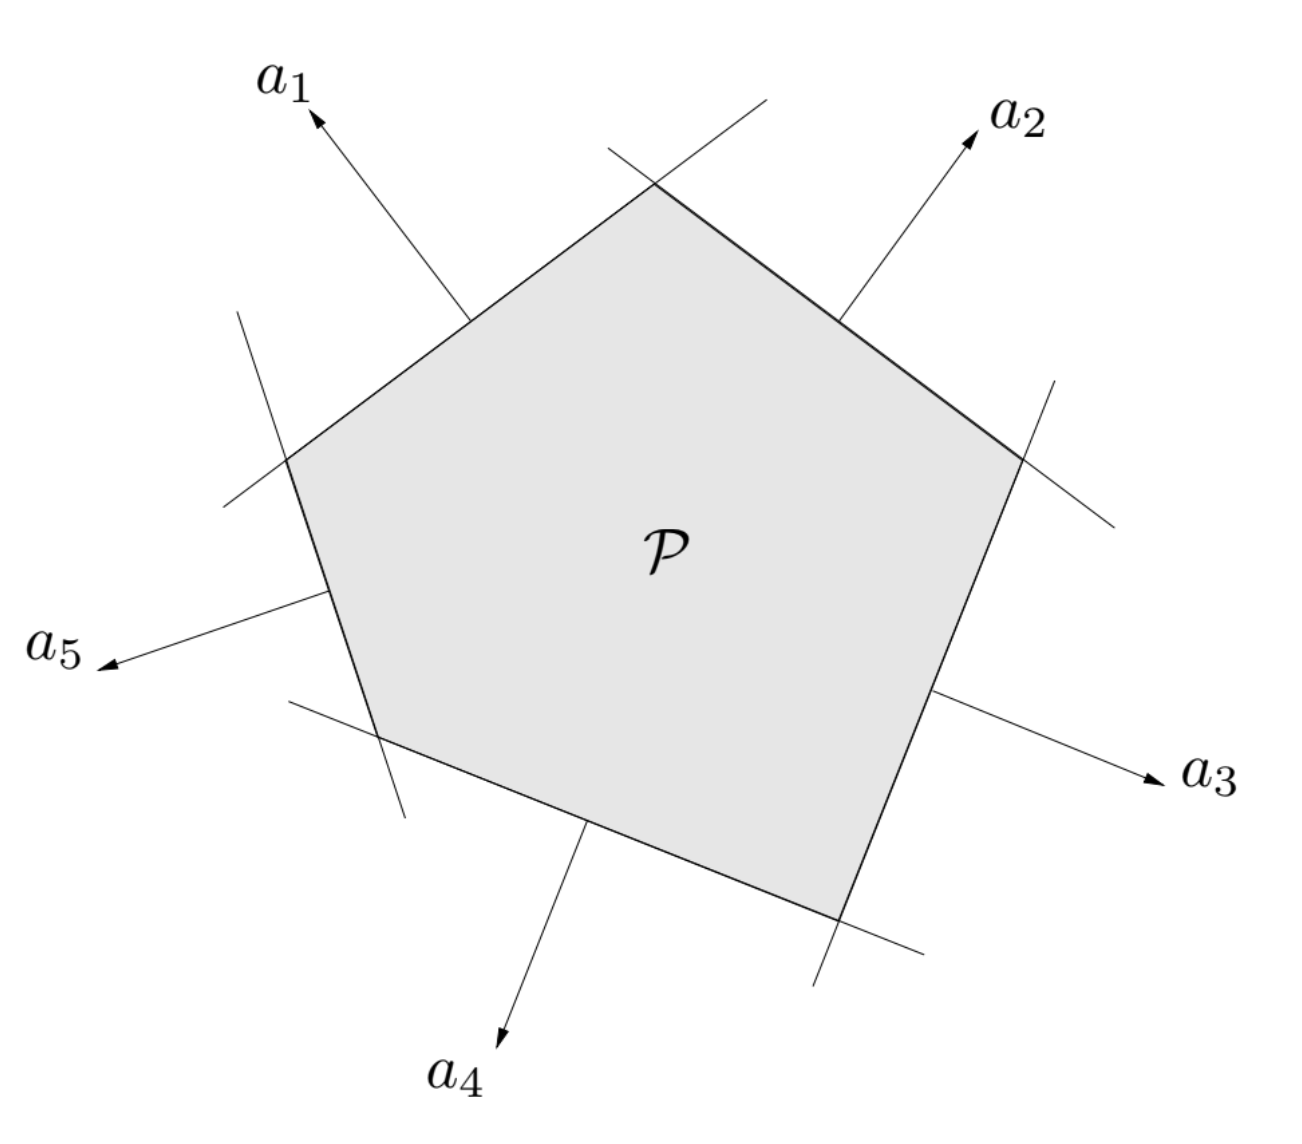
\includegraphics[width=0.3\textwidth]{Figs/polyhedron.png}
    \caption{Polytope}
\end{figure}

\begin{definition}{Convex set} \\
    A set $S \subseteq \mathbb{R}^n$ is convex if for all $x,y \in S$ and $\lambda \in [0,1]$, we have $\lambda t + (1- \lambda)y \in S$.
\end{definition}    

\begin{figure}[H]
    \centering
    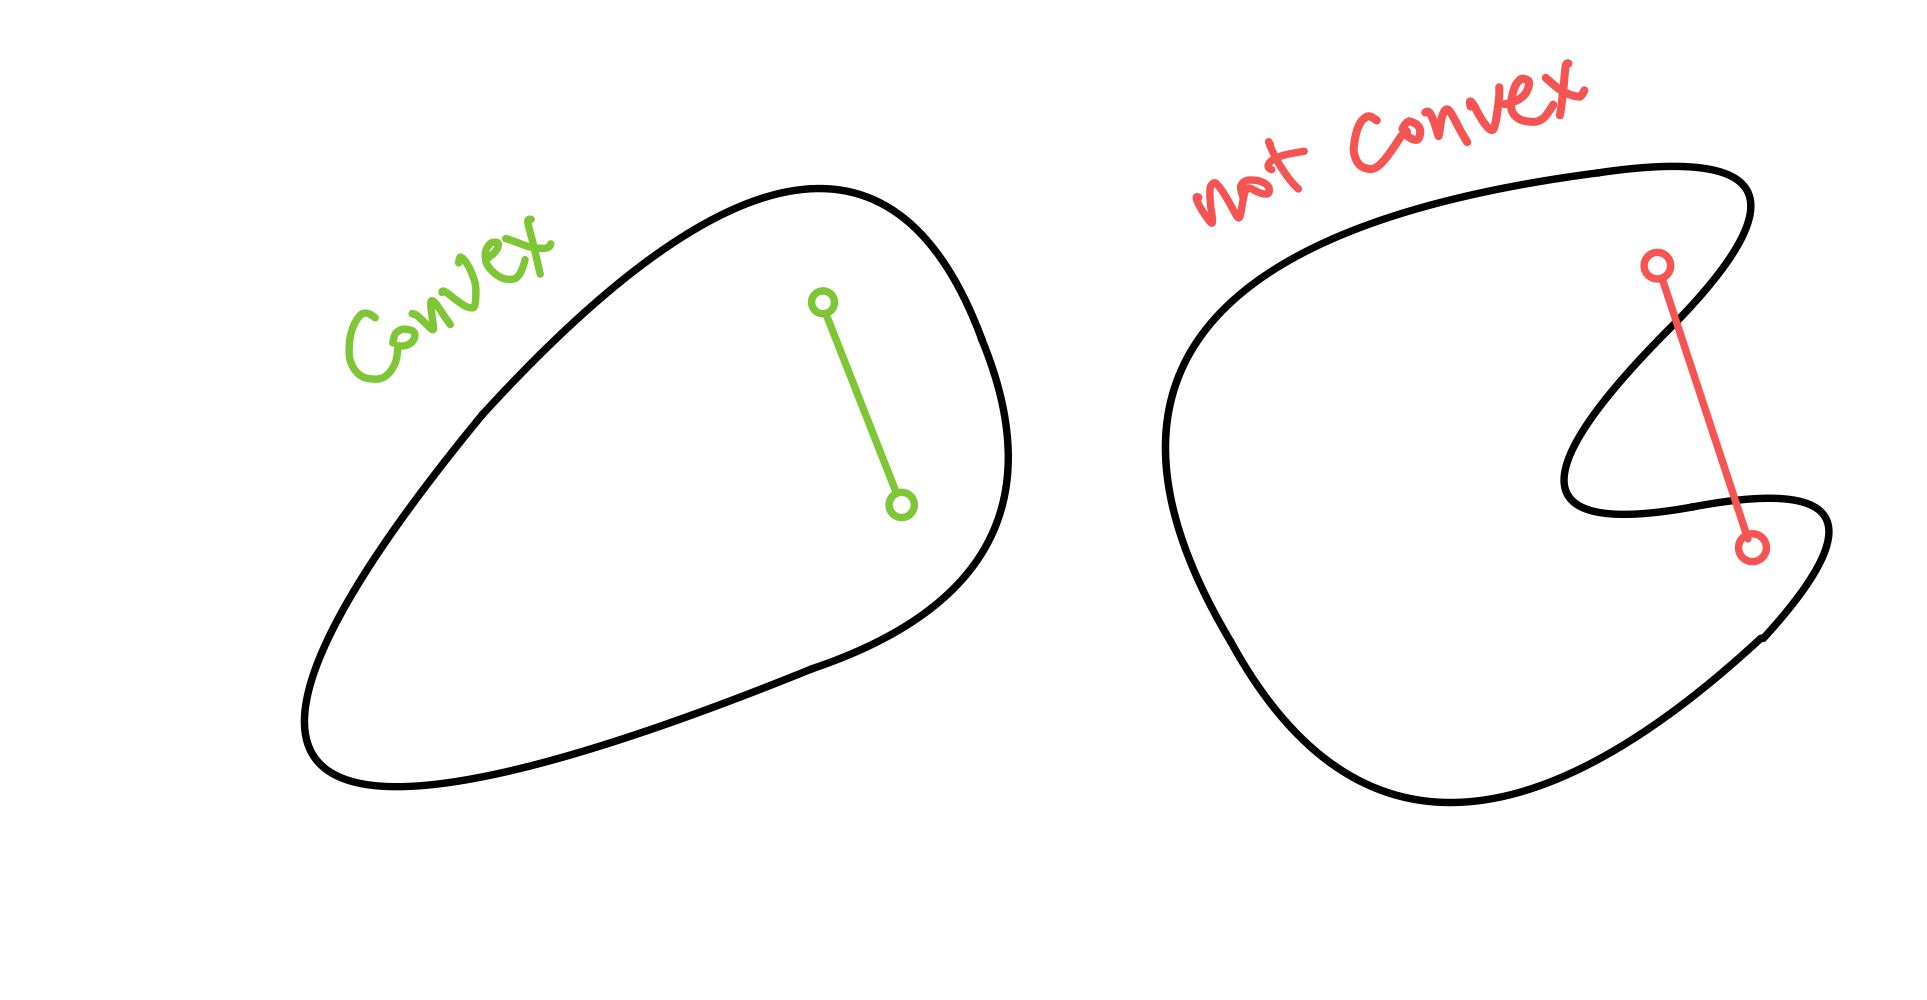
\includegraphics[width=0.5\textwidth]{Figs/convex_set.png}
    \caption{Convex set}
\end{figure}

\begin{definition}{Convex hull} \\
The convex hull of a set $S \subseteq \mathbb{R}^n$ is the smallest convex set that contains $S$.
\end{definition}


\begin{definition}{Conic combination} \\
A point $x \in \mathbb{R}^n$ is a conic combination of $y_1, \ldots, y_k \in \mathbb{R}^n$ 
if there exist $\lambda_1, \ldots, \lambda_k \geq 0$ such that $x = \sum_{i=1}^k \lambda_i y_i$.    
\end{definition}

\begin{definition}{Conic hull} \\
The conic hull of a finite set $S \subseteq \mathbb{R}^n$ is the set of all conic combinations of points in $S$.
\end{definition}


\begin{definition}{Convex cone} \\
A set $S \subseteq \mathbb{R}^n$ is a convex cone if for all $x \in S$ and $\lambda \geq 0$, we have $\lambda x \in S$.
\end{definition}

\begin{figure}[H]
    \begin{subfigure}{0.5\textwidth}
        \centering
        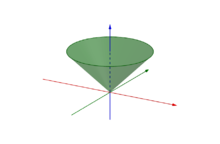
\includegraphics[width=\linewidth]{Figs/circular-pyramid.png}
        \caption{Convex cone that is not a conic hull of finitely many generators.}
    \end{subfigure}
    \begin{subfigure}{0.5\textwidth}
        \centering
        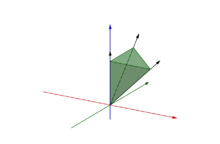
\includegraphics[width=\linewidth]{Figs/polyhedral_cone.png}
        \caption{Convex cone genrated by the conic combination of three black vectors (conic hull).}
    \end{subfigure}
\end{figure}

\begin{definition}{Normal cone} \\
The normal cone to a set $S$ at a point $x$ is defined as
\begin{equation}
    N_S(x) = \{ v \in \mathbb{R}^n : \langle v, y-x \rangle \leq 0 \text{ for all } y \in S \}
\end{equation}
\end{definition}

\begin{definition}{Tangent cone} \\
The tangent cone to a set $S$ at a point $x$ is defined as
\begin{equation}
    T_S(x) = \{ v \in \mathbb{R}^n : \lim_{t \rightarrow 0^+} \frac{x + tv - x}{t} \in S \}
\end{equation}
\end{definition}

\begin{figure}[H]
    \centering
    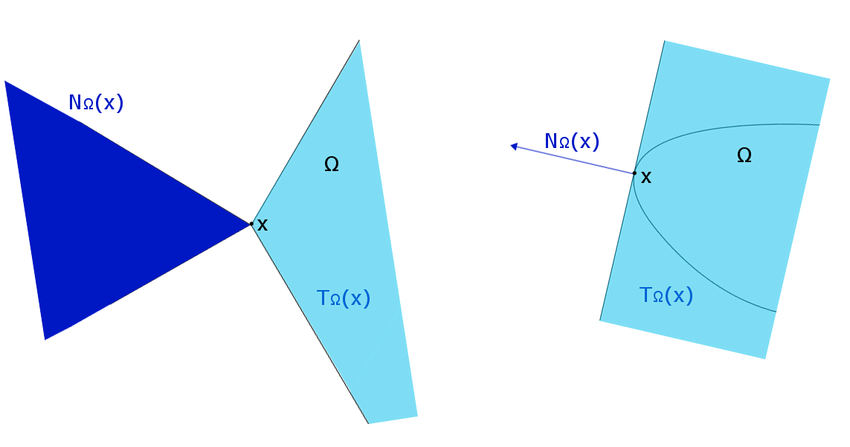
\includegraphics[width=0.5\textwidth]{Figs/normal-cones.png}
    \caption{Normal and tangent cones}
\end{figure}

\begin{theorem}{Normal cone of polyhedron} \\
The normal cone to a polyhedron $S = \{x \in \mathbb{R}^n : \forall j \in [m] \quad a_j \cdot x \leq b_j\}$ at a point $x$ is given by
\begin{equation}
    N_S(x) = \{ \sum_{j} \lambda_j a_j : \lambda_j \geq 0  \text{ and }  a_j \cdot x = b_j \}
\end{equation}
    
\end{theorem}


% * * * * * * * * * * * * * * * * * * * * * * * *
% * * * * * * * * * * * * * * * * * * * * * * * *
% * * * * * * * * * * * * * * * * * * * * * * * *
% * * * * * * * * * * * * * * * * * * * * * * * *
% * * * * * * * * * * * * * * * * * * * * * * * *
% * * * * * * * * * * * * * * * * * * * * * * * *
% * * * * * * * * * * * * * * * * * * * * * * * *


\section{Definitions and Fundamental Theorems}



\begin{definition} (Convex function): A function $f : S \rightarrow \mathbb{R}$ defined on a convex set $S$ is convex if, for all $x, y \in S$ and $\lambda \in [0,1]$, 
\[ f(\lambda x + (1-\lambda)y) \leq \lambda f(x) + (1-\lambda) f(y). \]
\end{definition}

\begin{figure}[H]
    \centering
    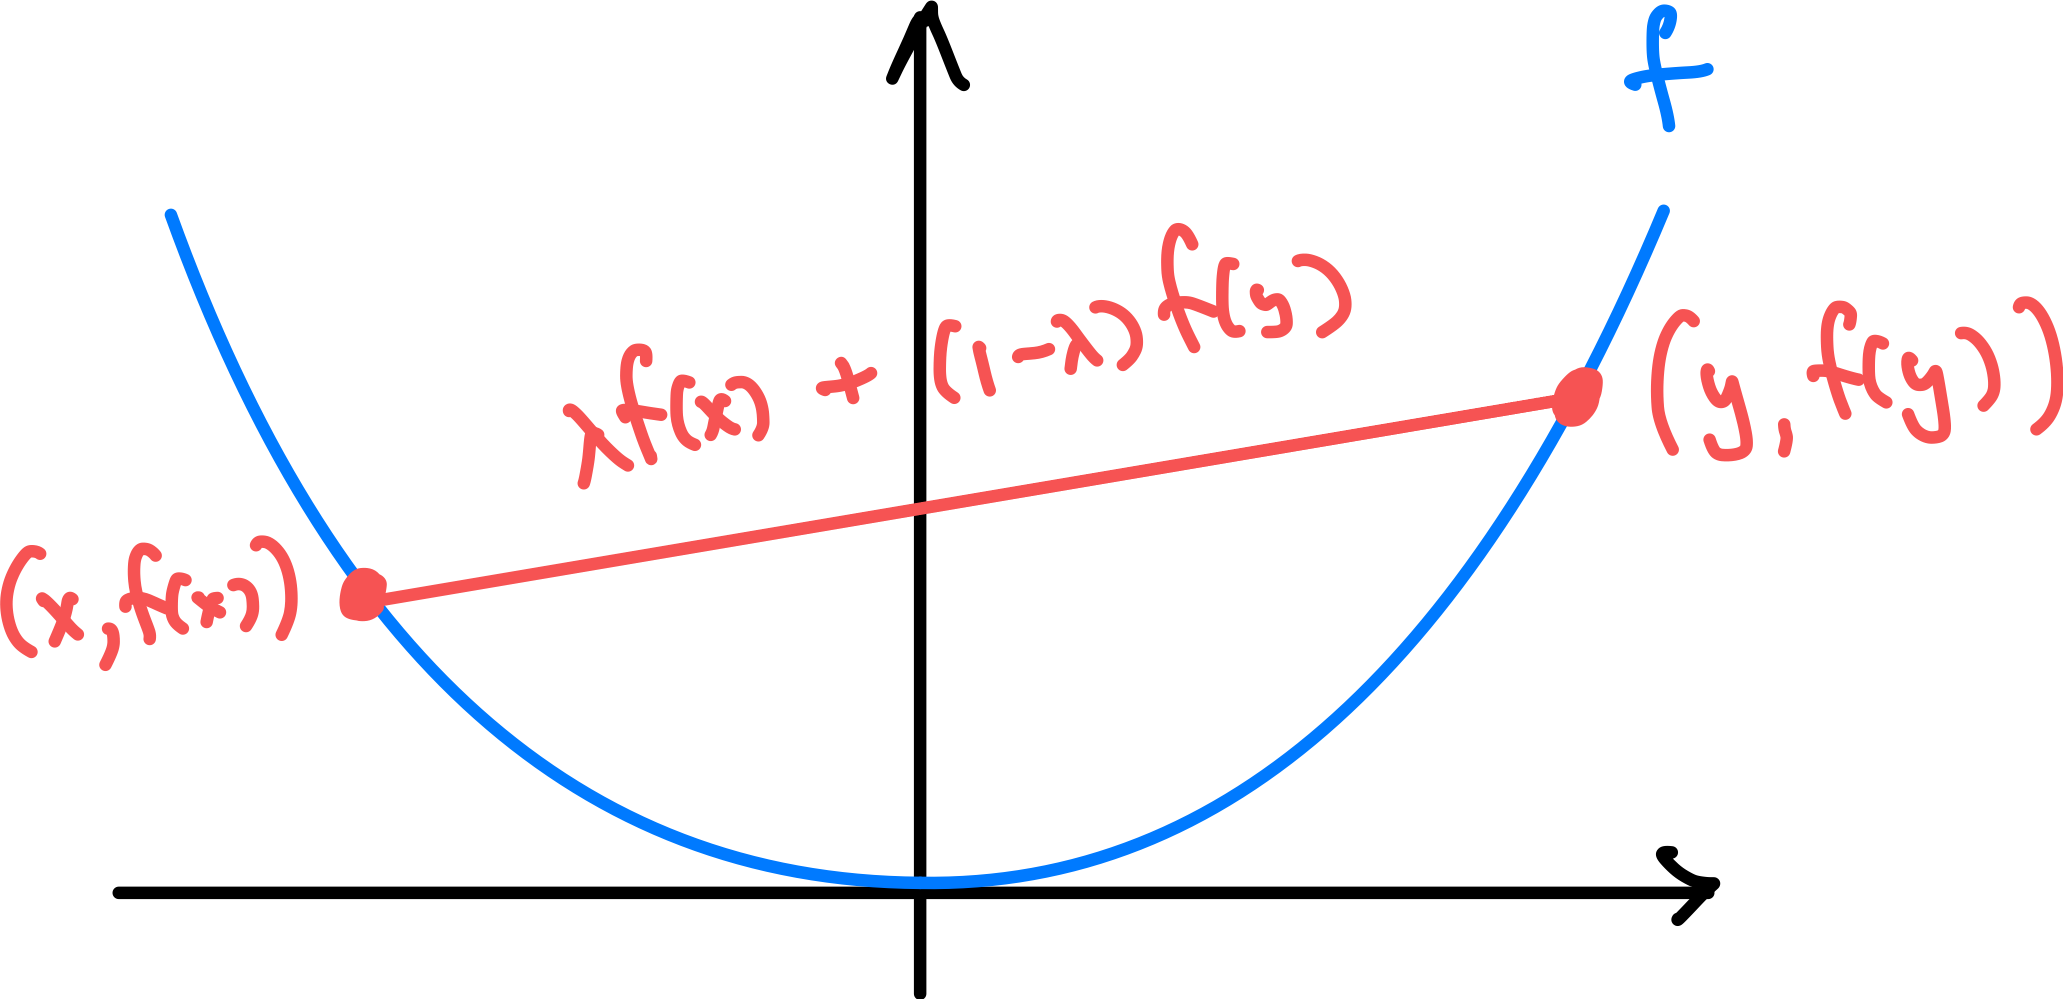
\includegraphics[width=0.5\textwidth]{Figs/convex_function.png}
    \caption{Convex function}
\end{figure}

\begin{theorem} (Characterization via epigraph): A function $f : S \to \mathbb{R}$ is convex if and only if its epigraph $\{(x,t) \in S \times \mathbb{R} : f(x) \leq t\}$ is a convex set.
\end{theorem}

\begin{figure}[H]
    \centering
    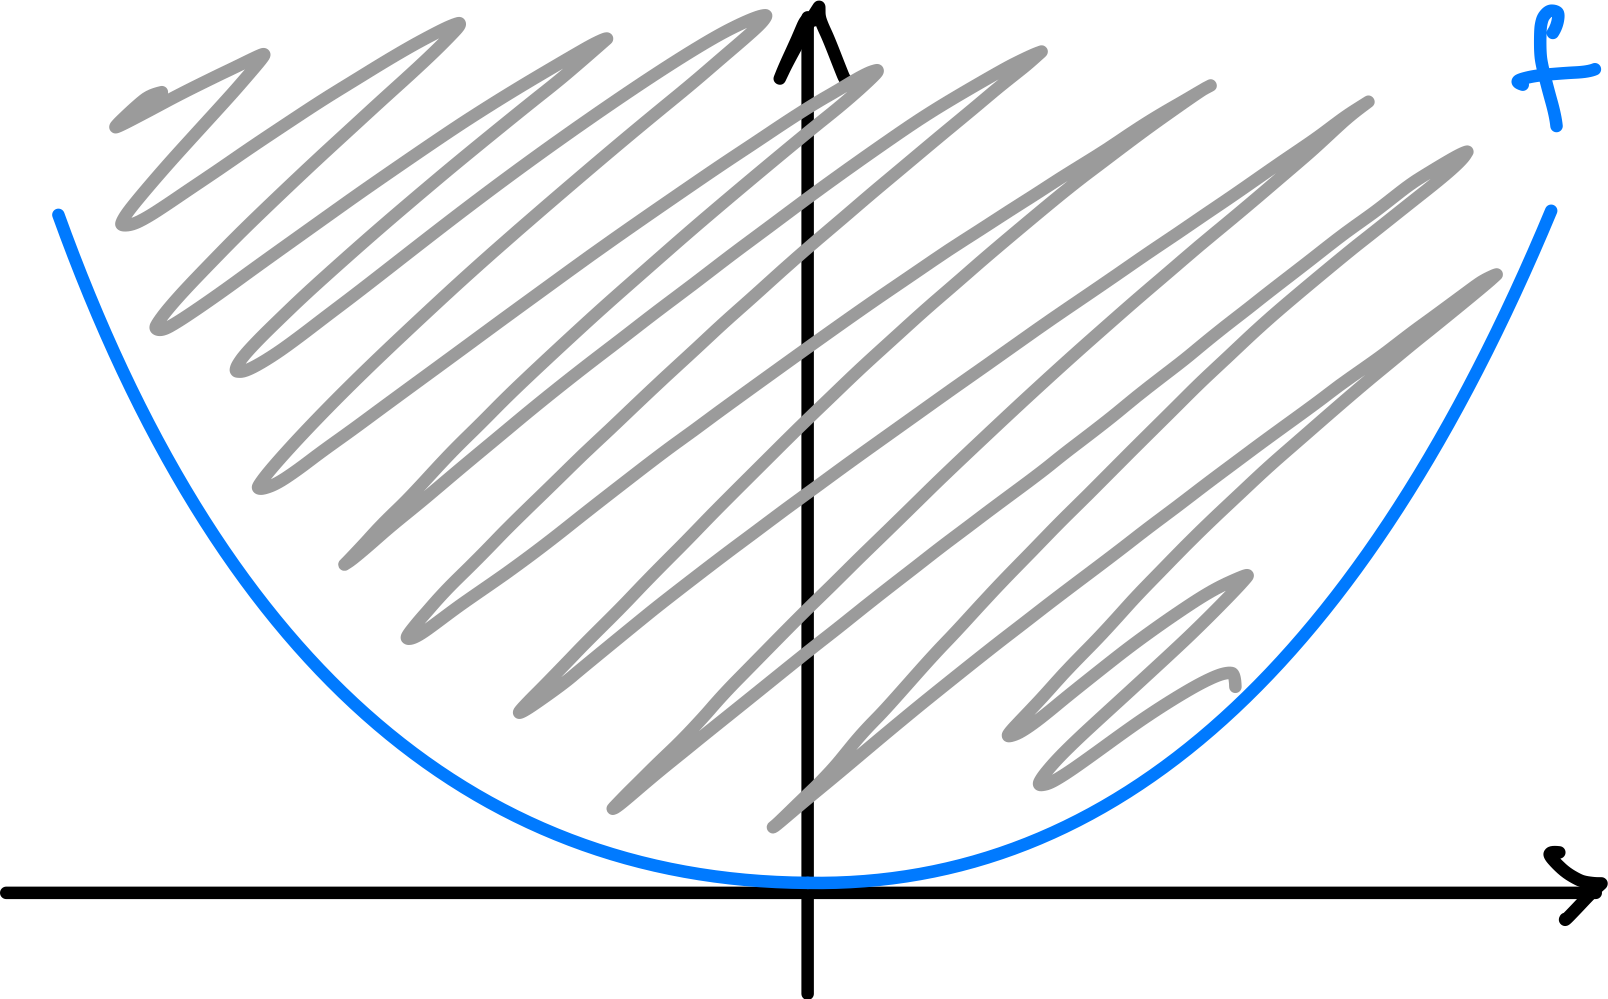
\includegraphics[width=0.3\textwidth]{Figs/epigraph_of_convex_function.png}
    \caption{Epigraph of a convex function}
\end{figure}


\begin{claim} (Convexity of sublevel sets): If $f : S \to \mathbb{R}$ is convex, then the sublevel set $S_t = \{ x \in S : f(x) \leq t\}$ is convex for any $t \in \mathbb{R}$.
\end{claim}

\section{Inequalities and Characterizations}

\begin{theorem}(Jensen's inequality): If $f$ is a convex function, then for any $x_1, x_2, \ldots, x_n \in S$ and any non-negative weights $\alpha_i$ such that $\sum_{i=1}^n \alpha_i = 1$,
\[ f\left(\sum_{i=1}^n \alpha_i x_i\right) \leq \sum_{i=1}^n \alpha_i f(x_i). \]
\end{theorem}


\begin{theorem}(First-order characterization, aka “the gradient inequality”): If $f$ is a differentiable convex function on an open set $S$, then for all $x, y \in S$,
\[ f(y) \geq f(x) + \nabla f(x)^\top (y - x). \]
\end{theorem}

\begin{figure}[H]
    \centering
    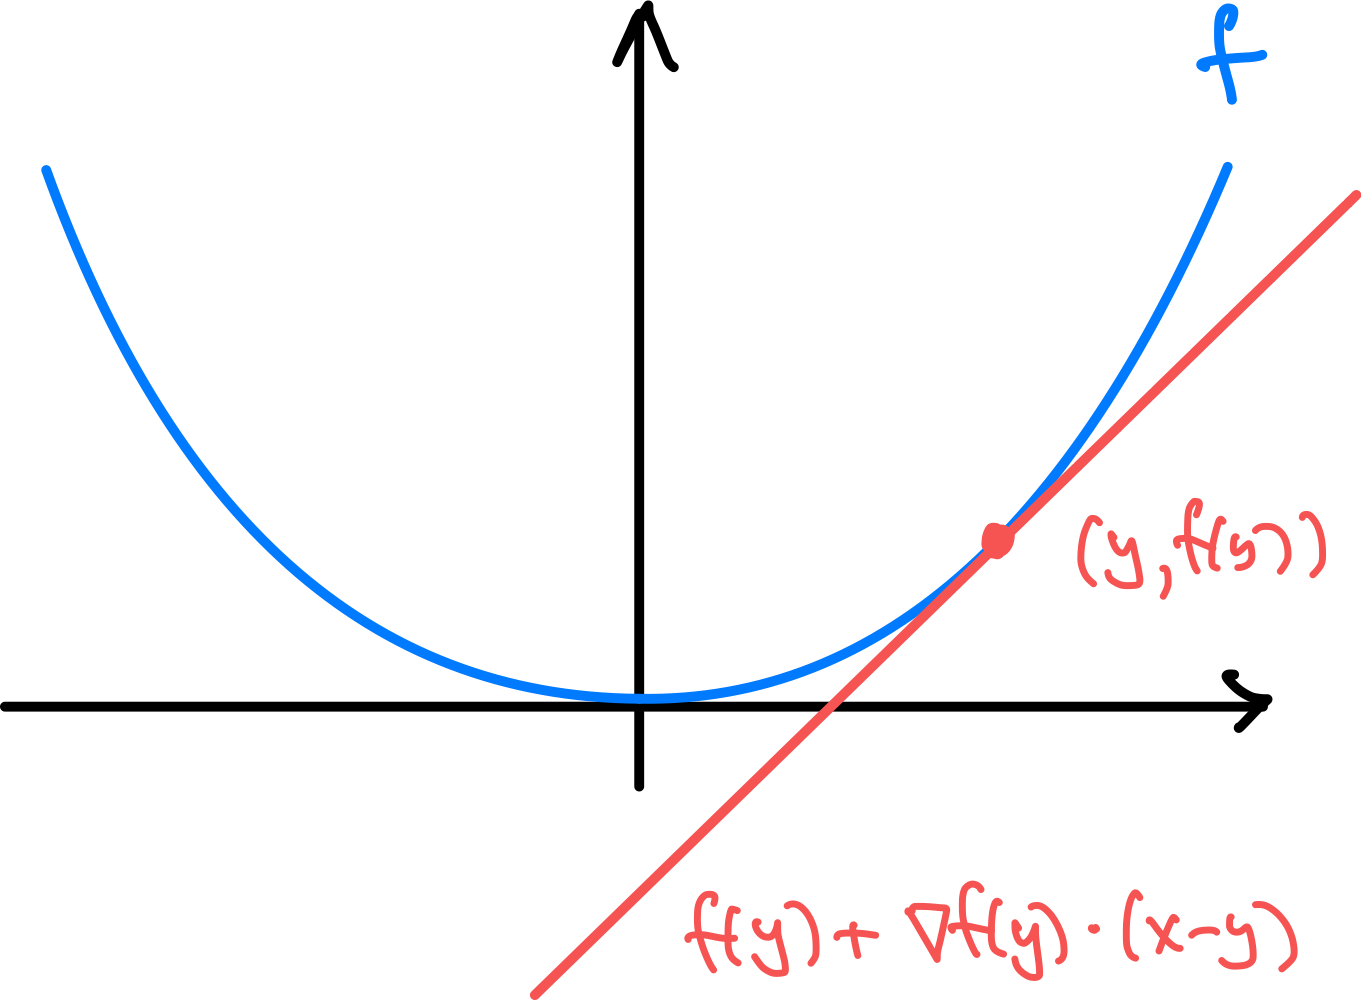
\includegraphics[width=0.3\textwidth]{Figs/first_order_characterization_of_convexity.png}
    \caption{First-order characterization of convexity}
\end{figure}

\begin{definition}{Bergman divergence (distance)} \\
The Bergman divergence between two points $x, y \in \mathbb{R}^n$ is defined as
\begin{equation}
    D_f(x,y) = f(x) - f(y) - \nabla f(y)^\top (x-y)
\end{equation}
\end{definition}


\begin{theorem} (Jensen’s inequality, generalized for expectation): If $f$ is a convex function and $X$ is a random variable over $S$, then
\[ f(\mathbb{E}[X]) \leq \mathbb{E}[f(X)]. \]
\end{theorem}


\begin{theorem} (Second-order characterization of convexity): A twice differentiable function $f$ is convex on an open set $S$ if and only if the Hessian matrix of $f$ is positive semidefinite at every point in $S$.
\end{theorem}

\section{Optimization and Projection}

\begin{definition} (Convex optimization): The problem of minimizing a convex function over a convex set.
\end{definition}

\begin{theorem} (Optimality conditions, unconstrained): If $f$ is convex and differentiable, \\
     $x^*$ is a local minimum of $f$ $\Leftrightarrow$ $x^*$ is a global minimum of $f$ $\Leftrightarrow$  $\nabla f(x^*) = 0$.
\end{theorem}

\begin{theorem} (Optimality conditions, constrained): If $f$ is differentiable and $C$ is a convex set,
     $x^*$ is a local minimum of $f$ on $C$ if and only if $\langle \nabla f(x^*), x - x^* \rangle \geq 0$ for all $x \in C$.
\end{theorem}

\begin{figure}[H]
    \centering
    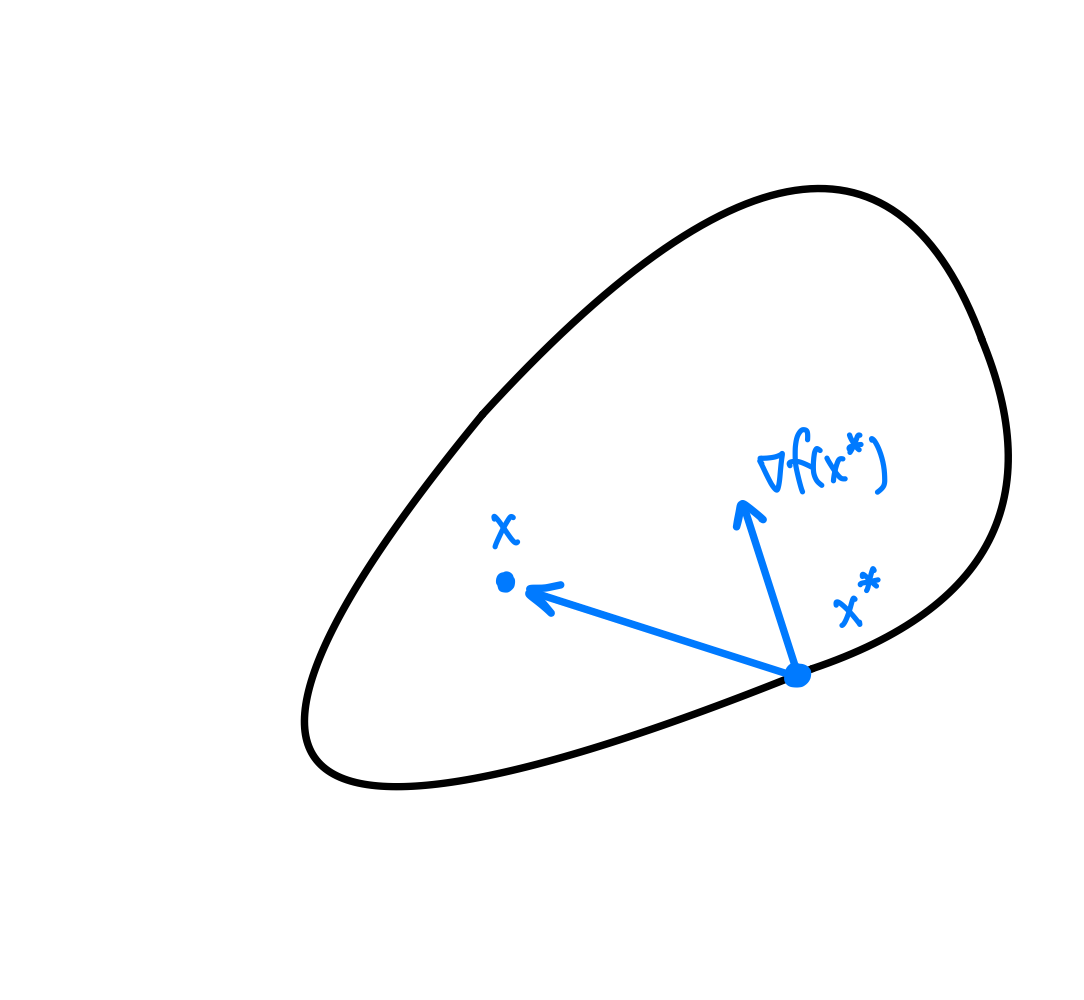
\includegraphics[width=0.5\textwidth]{Figs/optimality_condition_constrained.png}
    \caption{Optimality conditions, constrained}
\end{figure}


\begin{corollary}{Optimality conditions, constrained (alternative)} \\
If $f$ is differentiable and $C$ is a convex set, then $x^*$ is a local minimum of $f$ on $C$ if and only if $-\nabla f(x^*) \in N_C(x^*)$.
\end{corollary}

\begin{definition} (Projection): The projection of a point $x$ onto a convex set $S$ is defined as $\Pi_S(x) = \arg\min_{y \in S} \|y-x\|$.
\end{definition}

\begin{figure}[H]
    \centering
    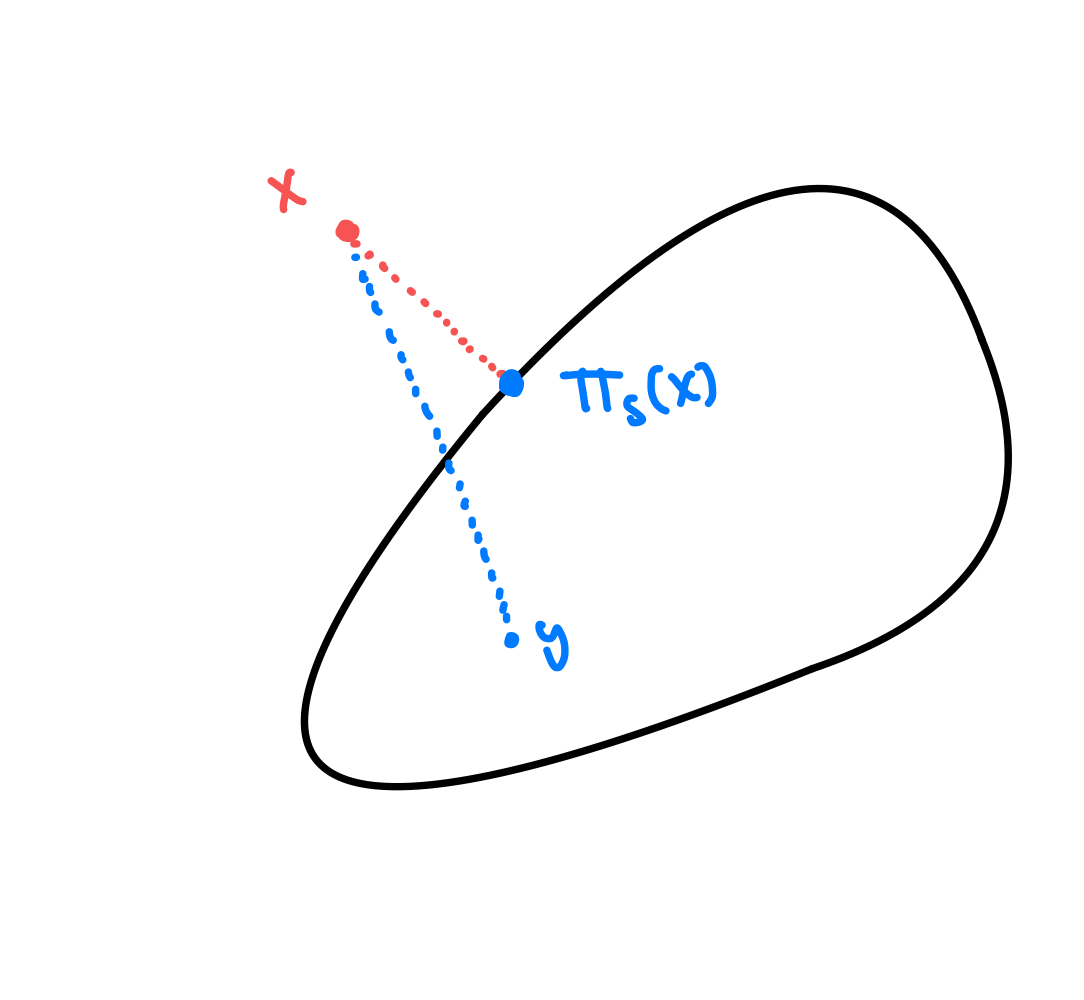
\includegraphics[width=0.3\textwidth]{Figs/projection.png}
    \caption{Projection}
\end{figure}


\begin{theorem} {Generalized cosine theorem} \\
    Let \( S \subseteq \mathbb{R}^d \) be convex and \( x \in \mathbb{R}^d \). Then the projection \( \Pi_S[x] \) is unique and satisfies:
    \begin{equation}
    \| x - \Pi_S[x] \|^2 + \| \Pi_S[x] - y \|^2 \leq \| x - y \|^2, \quad \forall y \in S.
    \end{equation}
    In particular:
    \begin{equation}
    \| \Pi_S[x] - y \| \leq \| x - y \|, \quad \forall y \in S.
    \end{equation}
\end{theorem}


% * * * * * * * * * * * * * * * * * * * * * * * *
% * * * * * * * * * * * * * * * * * * * * * * * *
% * * * * * * * * * * * * * * * * * * * * * * * *
% * * * * * * * * * * * * * * * * * * * * * * * *
% * * * * * * * * * * * * * * * * * * * * * * * *
% * * * * * * * * * * * * * * * * * * * * * * * *
% * * * * * * * * * * * * * * * * * * * * * * * *


\section{Smooth Optimization}
\todo[inline]{Add the definitions and remove unrelated content.}

\begin{definition}{L - Lipschitz continuous} \\
A function $f: S \rightarrow \mathbb{R}$ is L-Lipschitz continuous if for all $x, y \in S$,
\begin{equation}
    |f(x) - f(y)| \leq L ||x-y||
\end{equation}    
\end{definition}

\begin{theorem}{Convexity and Lipschitz continuity} \\
If $f$ is convex, differentiable and L-Lipschitz continuous, then $||\nabla f(x)|| \leq L$ for all $x \in S$. 
\end{theorem}

\begin{definition} {Smooth function} \\
    A differentiable function \( f \) is \(\beta\)-smooth over \( S \subseteq \text{dom} f \) if for all \( x, y \in S \):
    \[-\frac{\beta}{2} \|y - x\|^2 \leq f(y) - f(x) - \nabla f(x) \cdot (y - x) \leq \frac{\beta}{2} \|y - x\|^2.\]
\end{definition}


\begin{figure}[H]
    \centering
    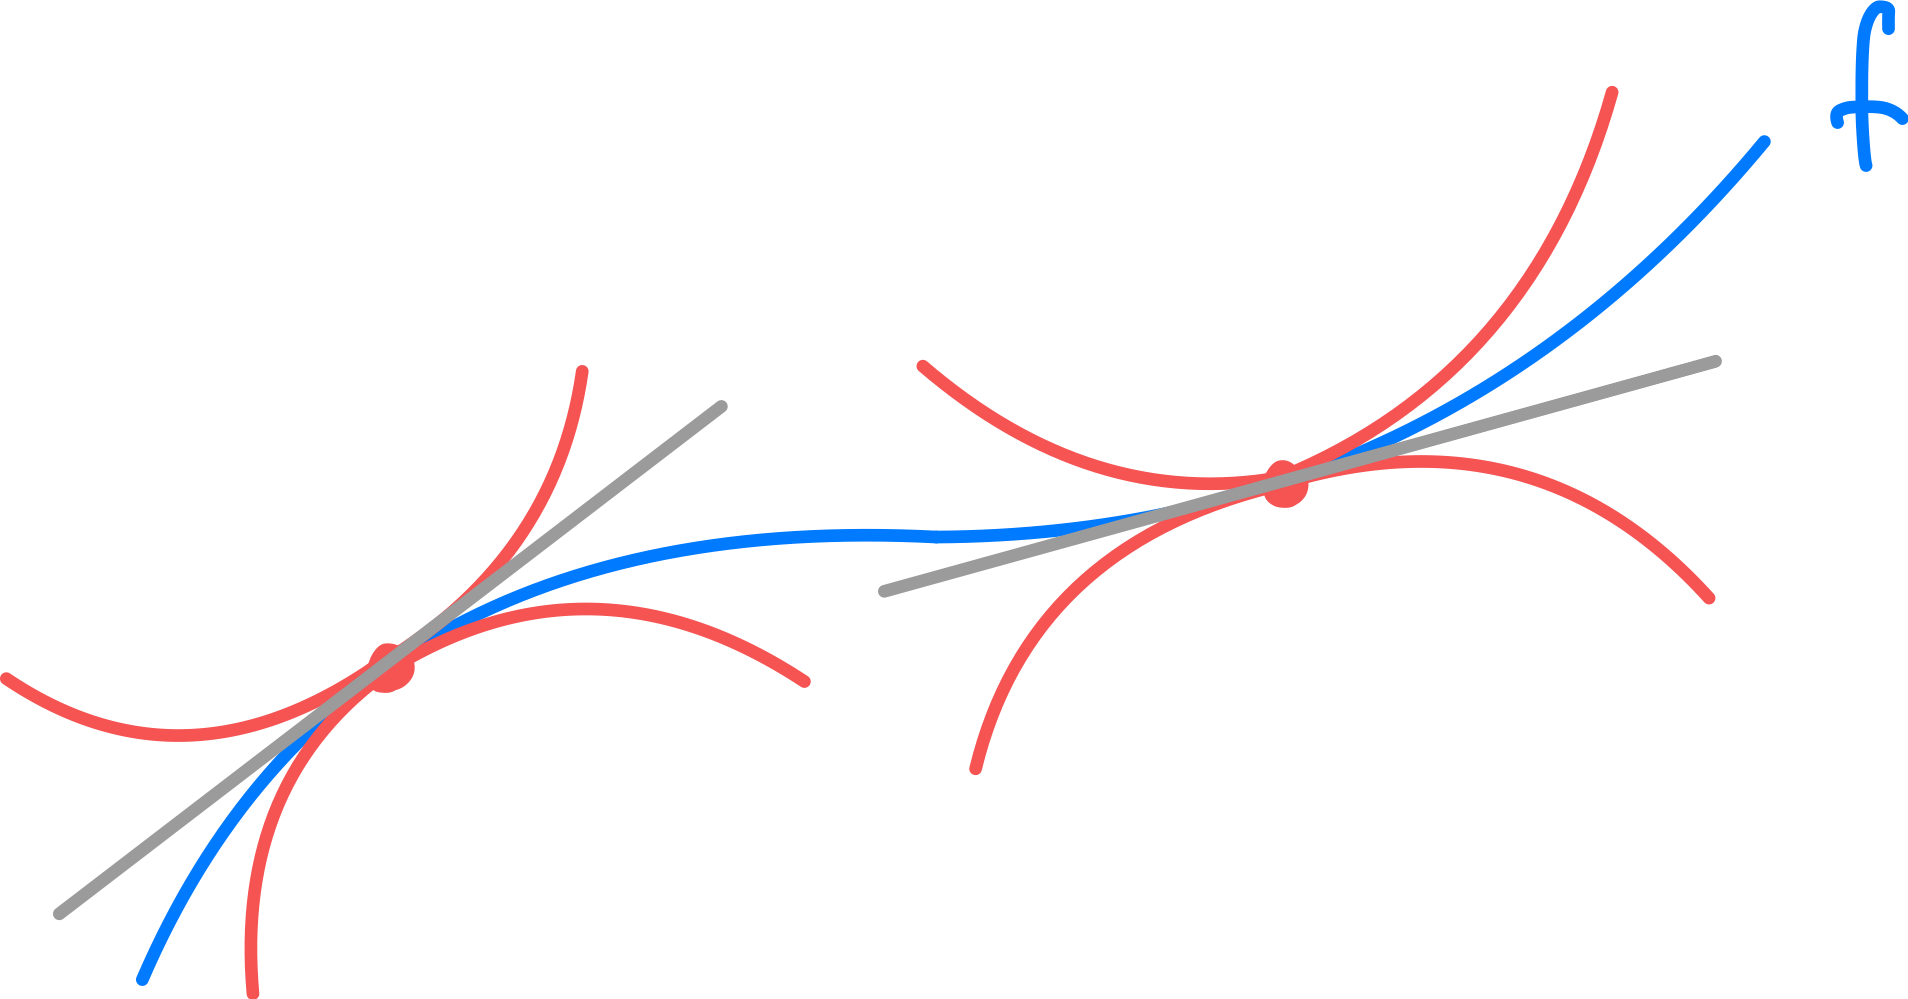
\includegraphics[width=0.7\textwidth]{Figs/beta_smooth_function.png}
    \caption{Smooth function}
\end{figure}


\begin{theorem} {Lipschitz gradient interpretation } \\
Let \( f \) be differentiable and let \( S \subseteq \text{dom} f \) be convex and closed. Suppose that
\[\|\nabla f(x) - \nabla f(y)\| \leq \beta \|x - y\|, \quad \forall x, y \in S.\]
Then \( f \) is \(\beta\)-smooth over \( S \).
\end{theorem}

\begin{theorem} {Second-order characterization of smoothness} \\
Let \( f \) be \( C^2 \) and let \( S \subseteq \text{dom} f \) be convex and closed. Then \( f \) is \(\beta\)-smooth over \( S \) if and only if
\[-\beta I \preceq \nabla^2 f(x) \preceq \beta I, \quad \forall x \in S.\]
\end{theorem}


\begin {lemma} {The Descent Lemma} \\
Let \( f : \mathbb{R}^d \rightarrow \mathbb{R} \) be \(\beta\)-smooth, and let \( x \in \mathbb{R}^d \).
\end{lemma}

\begin{itemize}
    \item For \( \eta \leq \frac{1}{\beta} \), \( x^{+} = x - \eta \nabla f(x) \), we have
    \[ f(x^{+}) - f(x) \leq -\frac{\eta}{2} \|\nabla f(x)\|^2. \]
    \item For \( x^{*} \in \text{arg\,min}_x f(x) \), we have
    \[ \frac{1}{2\beta} \|\nabla f(x)\|^2 \leq f(x) - f(x^{*}). \]
\end{itemize}

\textbf{Basic Facts}:
\begin{itemize}
    \item An affine function \( f : \mathbb{R}^d \rightarrow \mathbb{R}, f(x) = a^\top x + b \), is 0-smooth.
    \item A quadratic function \( f : \mathbb{R}^d \rightarrow \mathbb{R}, f(x) = \frac{1}{2} x^\top A x + b^\top x + c \), is \( \lambda_{\text{max}}(A) \)-smooth.
    \item A linear combination of smooth functions is smooth with an appropriate parameter.
    \item A convex combination of \(\beta\)-smooth functions is \(\beta\)-smooth.
\end{itemize}

\subsubsection{"Proximal" view of smooth optimization}

Our initial motivation for introducing smoothness was for ensuring that the gradient $\nabla f(x_t)$ 
(used in the optimization step) is indeed a faithful representative of the local behavior of the objective $f$ around $x_t$.

We formalized this by a requirement that the linear approximation of $f$ at $x_t$ is not too far from $f$ close to $x_t$: 
\[
f(x) \leq f(x_t) + \nabla f(x_t) \cdot (x - x_t) + \frac{\beta}{2} \|x - x_t\|^2.
\]
(We ignore the symmetric lower bound since we are still focusing on convex $f$.)

Revisiting this approach, a tempting idea is to use this approximation of $f$ for algorithm design: since it is easy to minimize a quadratic, we can try to construct $x_{t+1}$ by minimizing the RHS of the upper bound above.

\begin{figure}[H]
    \centering
    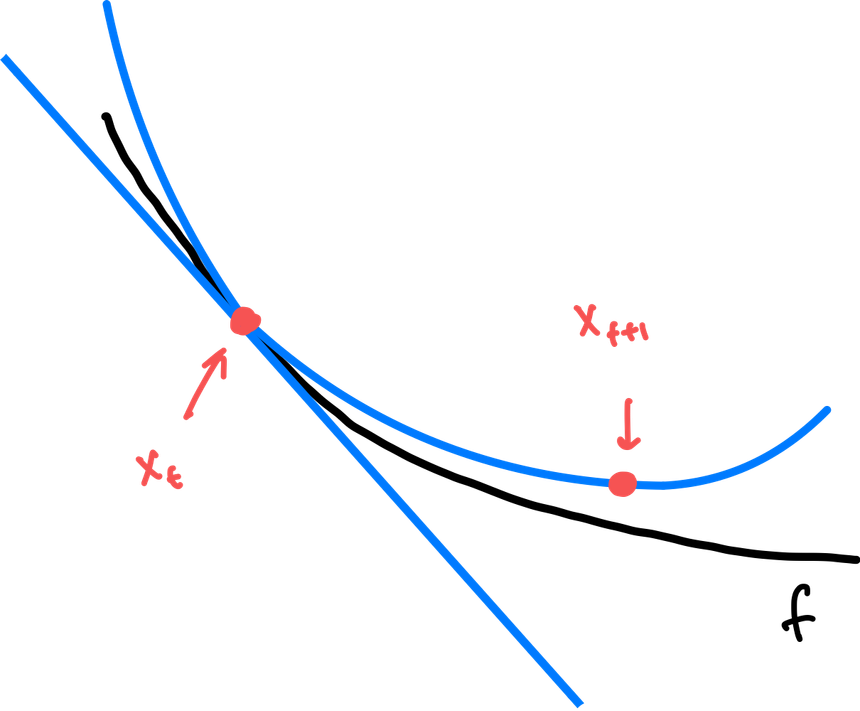
\includegraphics[width=0.4\textwidth]{Figs/proximal_view_of_smooth_optimization.png}
    \caption{Proximal view of smooth optimization}
\end{figure}

To solve this, let's take the gradient with respect to \( y \) and equate to zero:
\[
\nabla f(x_t) + \beta (x_{t+1} - x_t) = 0 \Rightarrow x_{t+1} = x_t - \frac{1}{\beta} \nabla f(x_t).
\]
This precisely gives gradient descent with \( \eta = \frac{1}{\beta} \)!

\begin{remark*}{\textbf{Gradient Descent as Proximal Operator}} \\
    Given a convex and \(\beta\)-smooth \( f \colon \mathbb{R}^d \rightarrow \mathbb{R} \) and starting from \( x_1 \in \mathbb{R}^d \), compute for \( t = 1, 2, \dots \):
    \[
    x_{t+1} = \arg\min_{x \in \mathbb{R}^d} \left\{ f(x_t) + \nabla f(x_t) \cdot (x - x_t) + \frac{\beta}{2} \| x - x_t \|^2 \right\}.
     \]
\end{remark*}

\medbreak

This motivates the following definition, central to convex optimization:

\begin{definition}{\textbf{Proximal operator (``prox'')}} \\
    The proximal operator associated with a convex function \( h \colon \mathbb{R}^d \rightarrow \mathbb{R} \) is:
    \[
    \text{prox}_{h,\eta}(x) = \arg\min_{y \in \mathbb{R}^d} \left\{ h(y) + \frac{1}{2\eta} \| y - x \|^2 \right\}
    \]
\end{definition}

Thus, a step of (unconstrained) gradient descent can be viewed as a proximal operator
\[
x_{t+1} = \text{prox}_{h_t, 1/\beta}(x_t),
\]
applied to a linearization \( h_t \) of \( f \) at \( x_t \):
\[
h_t(x) = f(x_t) + \nabla f(x_t) \cdot (x - x_t).
\]

A similar equivalence also holds in the constrained case.




% * * * * * * * * * * * * * * * * * * * * * * * *
% * * * * * * * * * * * * * * * * * * * * * * * *
% * * * * * * * * * * * * * * * * * * * * * * * *
% * * * * * * * * * * * * * * * * * * * * * * * *
% * * * * * * * * * * * * * * * * * * * * * * * *
% * * * * * * * * * * * * * * * * * * * * * * * *
% * * * * * * * * * * * * * * * * * * * * * * * *


\section{Strong Convexity}
\todo[inline]{Add the definitions and remove unrelated content.}


\begin{definition} {Strong convexity} \\
A function \( f \) is \(\alpha\)-strongly convex (for \(\alpha \geq 0\)) over a convex and closed set \( S \subseteq \text{dom} f \) if for any \( x \in S \), there exists \( g_x \in \partial f(x) \) such that:
\[
\forall y \in S, \quad f(y) \geq f(x) + g_x \cdot (y - x) + \frac{\alpha}{2} \|y - x\|^2.
\]
In particular, a differentiable \( f \) is \(\alpha\)-strongly convex over \( S \) if for any \( x \in S \),
\[
\forall y \in S, \quad f(y) \geq f(x) + \nabla f(x) \cdot (y - x) + \frac{\alpha}{2} \|y - x\|^2.
\]
\end{definition}

\begin{figure}[H]
    \centering
    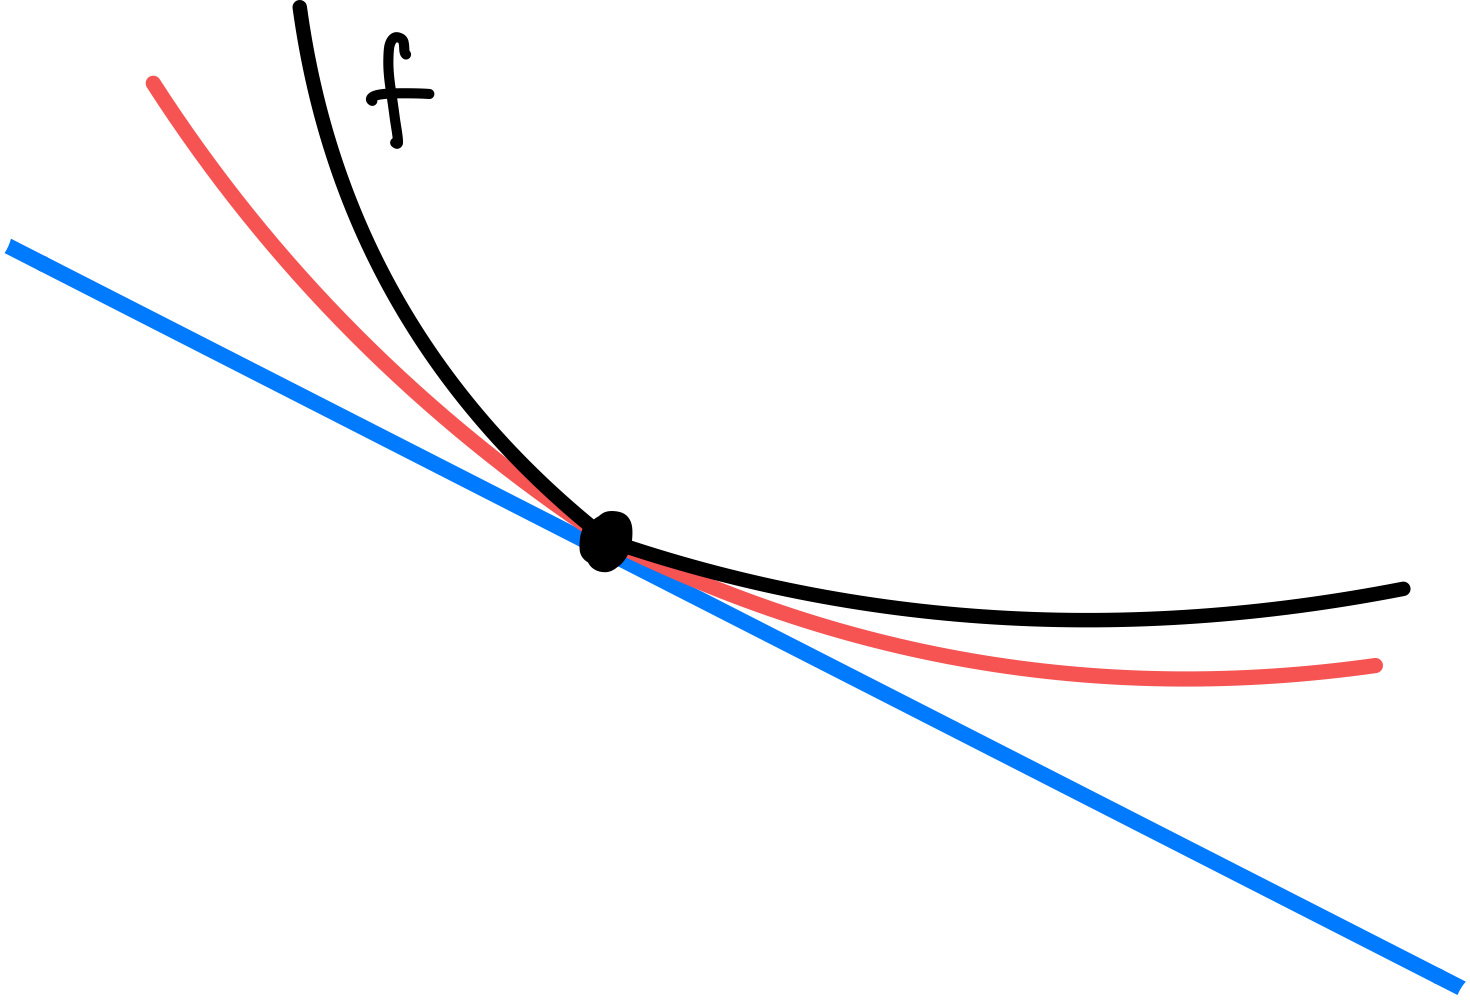
\includegraphics[width=0.5\textwidth]{Figs/strongly_convex.png}
    \caption{Strongly convex function}
\end{figure}

\begin{theorem} { Strong convexity, second-order characterization}\\
Let \( f \) be \( C^2 \) and let \( S \subseteq \text{dom} f \) be convex and closed. Then \( f \) is \(\alpha\)-strongly convex over \( S \) if and only if
\[
\forall x \in S, \quad \nabla^2 f(x) \succeq \alpha I.
\]
\end{theorem}


\begin{theorem} {Usage of strong convexity } \\
If a differentiable \( f \) is \(\alpha\)-strongly convex over a convex and closed \( S \subseteq \text{dom} f \) with a minimum at \( x^* \in S \), then
\[
\forall x \in S, \quad \frac{\alpha}{2} \|x - x^*\|^2 \leq f(x) - f(x^*) \leq \frac{1}{2\alpha} \|\nabla f(x)\|^2.
\]
In particular, the minimum of a strongly convex function is unique.
\end{theorem}

% * * * * * * * * * * * * * * * * * * * * * * * *
% * * * * * * * * * * * * * * * * * * * * * * * *
% * * * * * * * * * * * * * * * * * * * * * * * *
% * * * * * * * * * * * * * * * * * * * * * * * *
% * * * * * * * * * * * * * * * * * * * * * * * *
% * * * * * * * * * * * * * * * * * * * * * * * *
% * * * * * * * * * * * * * * * * * * * * * * * *


\section{}


% * * * * * * * * * * * * * * * * * * * * * * * *
% * * * * * * * * * * * * * * * * * * * * * * * *
% * * * * * * * * * * * * * * * * * * * * * * * *
% * * * * * * * * * * * * * * * * * * * * * * * *
% * * * * * * * * * * * * * * * * * * * * * * * *
% * * * * * * * * * * * * * * * * * * * * * * * *
% * * * * * * * * * * * * * * * * * * * * * * * *


\section{Important Inequalities}

\begin{theorem}{$1 + x \leq e^x$} \\
For all $x \in \mathbb{R}$, we have $1 + x \leq e^x$.    
\end{theorem}

\begin{proof}
Let $f(x) = e^x - 1 - x$. Then $f'(x) = e^x - 1$ and $f''(x) = e^x > 0$. Thus, $f$ is convex and $f(0) = 0$. Therefore, $f(x) \geq 0$ for all $x \in \mathbb{R}$.
\end{proof}

\begin{figure}[H]
    \centering
    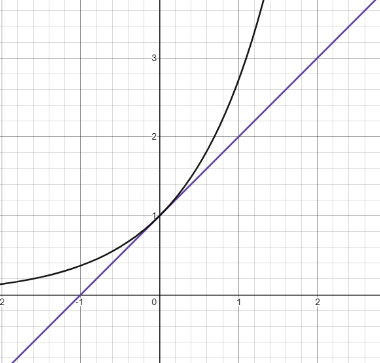
\includegraphics[width=0.3\textwidth]{Figs/1+x_leq_e^x.png}
    \caption{$1 + x \leq e^x$}
\end{figure}


% * * * * * * * * * * * * * * * * * * * * * * * * 
% * * * * * * * * * * * * * * * * * * * * * * * * 
% * * * * * * * * * * * * * * * * * * * * * * * * 
% * * * * * * * * * * * * * * * * * * * * * * * * 
% * * * * * * * * * * * * * * * * * * * * * * * * 
% * * * * * * * * * * * * * * * * * * * * * * * * 
% * * * * * * * * * * * * * * * * * * * * * * * * 
% * * * * * * * * * * * * * * * * * * * * * * * * 
% * * * * * * * * * * * * * * * * * * * * * * * * 
% * * * * * * * * * * * * * * * * * * * * * * * * 
% * * * * * * * * * * * * * * * * * * * * * * * * 
% * * * * * * * * * * * * * * * * * * * * * * * * 
% * * * * * * * * * * * * * * * * * * * * * * * * 
% * * * * * * * * * * * * * * * * * * * * * * * * 
% * * * * * * * * * * * * * * * * * * * * * * * * 
% * * * * * * * * * * * * * * * * * * * * * * * * 
% * * * * * * * * * * * * * * * * * * * * * * * * 
% * * * * * * * * * * * * * * * * * * * * * * * * 
% * * * * * * * * * * * * * * * * * * * * * * * * 



\chapter{Topology and manifolds}

\section{Metric space and complete metric space}

\begin{definition}{\textbf{Metric Space}} \\
    A metric space is a set \( X \) equipped with a metric, which is a function that defines a distance between each pair of elements in \( X \), satisfying the following properties for all \( x, y, z \in X \):
    \begin{enumerate}
        \item Non-negativity: \( d(x, y) \geq 0 \) and \( d(x, y) = 0 \) if and only if \( x = y \)
        \item Symmetry: \( d(x, y) = d(y, x) \)
        \item Triangle inequality: \( d(x, y) + d(y, z) \geq d(x, z) \)
    \end{enumerate}
\end{definition}

\( \textbf{Inner Product Space vs Metric Space} \)
\begin{itemize}
    \item An inner product space is a vector space equipped with an inner product, which is a function that associates each pair of vectors with a scalar.
    \item A metric space is a set equipped with a metric, which is a function that defines a distance between each pair of elements in the set.
    \item Every inner product space is a metric space, but not every metric space is an inner product space.
        \begin{example*}
            Each inner product space must satisfy the Parallelogram Law, which states that for all \( u, v \) in the space, \( 2\|u\|^2 + 2\|v\|^2 = \|u + v\|^2 + \|u - v\|^2 \).
            A clasic example of a metric space that is not an inner product space is the space of continuous functions on the interval \([0, 1]\) with the metric \( d(f, g) = \max_{x \in [0, 1]} |f(x) - g(x)| \).
        \end{example*}
\end{itemize}

\begin{definition}{ \textbf{Open $\epsilon$-ball} } \\
    Let \( (X, d) \) be a metric space and \( x \in X \). \\
    The open \(\varepsilon\)-ball centered at \( x \) is the set \(  B(x, \varepsilon) = \{ y \in X : d(x, y) < \varepsilon \} \).
\end{definition}

\begin{definition}{ \textbf{Open set} (metric space) } \\
    A subset \( U \) of a metric space \( (X, d) \) is open if for every point \( x \in U \), 
    there exists an open \(\varepsilon\)-ball centered at \( x \) that is contained in \( U \).
\end{definition}

\begin{definition}{\textbf{Convergence of a sequence}} \\
    A sequence \( (x_n) \) in a metric space \( (X, d) \) is said to \emph{converge} to a limit \( a \in X \) if, for every positive real number \( \varepsilon > 0 \),
    there exists a positive integer \( N \) such that for all positive integers \( n \geq N \), \( x_n \in B_{\varepsilon}(a) \).
\end{definition}

\begin{definition}{\textbf{Cauchy Sequence}} \\
    In a metric space \( (X, d) \), a sequence \( \{x_1, x_2, x_3, \ldots\} \) is said to be \emph{Cauchy} if, for every positive real number \( \varepsilon > 0 \),
     there exists a positive integer \( N \) such that for all positive integers \( m, n > N \), the distance
    \[ d(x_m, x_n) < \varepsilon. \]
\end{definition}

\begin{figure}[H]
    \begin{subfigure}{0.5\textwidth}
        \centering
        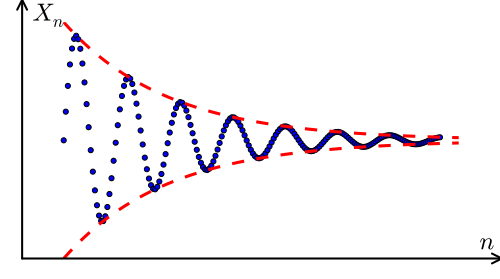
\includegraphics[width=0.45\textwidth]{Figs/Cauchy_sequence_illustration.png}
        \caption{The plot of a Cauchy sequence \( (x_n) \) shown in blue, as \( x_n \) versus \( n \). If the space is complete, then the sequence has a limit.}
    \end{subfigure}
    \hfill
    \begin{subfigure}{0.45\textwidth}
        \centering
        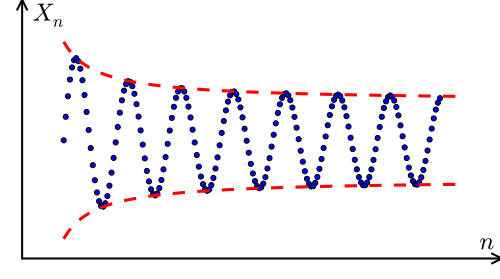
\includegraphics[width=0.5\textwidth]{Figs/Cauchy_sequence_illustration2.png}
        \caption{A sequence that is not Cauchy. The elements of the sequence do not get arbitrarily close to each other as the sequence progresses.}
    \end{subfigure}
    \caption{Cauchy Sequence}
\end{figure}

\begin{definition}{\textbf{Complete Metric Space}} \\
    A metric space is complete if every Cauchy sequence in the space converges to a limit in the space.
\end{definition}

\subsubsection{Hilbert Space}

\begin{definition}{\textbf{Hilbert Space}} \\
    A \emph{Hilbert space} is a complete inner product space. That is, it is an inner product space \( \mathcal{H} \) that 
    is also a complete metric space with respect to the metric induced by its inner product. 
    The metric is given by \( d(x,y) = \sqrt{\langle x-y, x-y \rangle} \) for all \( x, y \in \mathcal{H} \).
\end{definition}
    
A Hilbert space generalizes the notion of Euclidean space to an infinite-dimensional context. 
In a Hilbert space, one can still use concepts like angle, orthogonality, and projection, which are crucial in many areas of mathematics and physics. 
Completeness is a key feature of Hilbert spaces, meaning that every Cauchy sequence in the space converges to a limit within the space. 
    

% * * * * * * * * * * * * * * * * * * * * * * * *
% * * * * * * * * * * * * * * * * * * * * * * * *
% * * * * * * * * * * * * * * * * * * * * * * * *
% * * * * * * * * * * * * * * * * * * * * * * * *
% * * * * * * * * * * * * * * * * * * * * * * * *
% * * * * * * * * * * * * * * * * * * * * * * * *
% * * * * * * * * * * * * * * * * * * * * * * * *


\section{Topological Space}

\begin{definition}{\textbf{Topology}} \\
A topology \( \mathcal{T} \) on a set \( X \) is a collection of subsets of  \( X \) that satisfy the following properties:
\begin{enumerate}
    \item \( \emptyset, X \in \mathcal{T} \).
    \item The intersection of any finite number of sets is in \( \mathcal{T} \) - \\ 
    \( U_1, U_2, \ldots, U_n \in \mathcal{T} \) implies \( \bigcap_{i=1}^n U_i \in \mathcal{T} \).
    \item The union of any number of sets (finite or infinite) is in \( \mathcal{T} \) - \\
    \( U_\alpha \in \mathcal{T} \) for all \( \alpha \) in some index set \( A \) implies \( \bigcup_{\alpha \in A} U_\alpha \in \mathcal{T} \).
\end{enumerate}
\end{definition}

\begin{definition}{\textbf{Topological Space}} \\
A topological space is a pair \( (X, \mathcal{T}) \) consisting of a set \( X \) and a topology \( \mathcal{T} \) on \( X \).
\end{definition}

A metric space \( (X, d) \) induces a topology on \( X \) by defining the open sets to be the unions of open \( \varepsilon \)-balls centered at each point in \( X \). 

\begin{example*}
Examples of topological spaces:
\begin{enumerate}
    \item \( X = {1, 2, 3} \) with the topology \( T = \{\varnothing , \{1\}, \{1, 2\}, \{1, 2, 3\} \} \).
    \item Given any set $X$, \textbf{the discrete topology} on $X$ is the power set of $X$ - $\mathcal{T} = P(X)$ and is the largest possible topology on $X$.
    \item \textbf{The indiscrete topology} on $X$ is $\mathcal{T} = \{\emptyset, X\}$ and is the smallest possible topology on $X$ - 
    $\forall \mathcal{T}$, $\{\emptyset, X\} \subseteq \mathcal{T} \subseteq P(X)$.
    \item The real line \( \mathbb{R} \) with the standard topology.
    \item The set of integers \( \mathbb{Z} \) with the discrete topology.
    \item The set of real numbers \( \mathbb{R} \) with the lower limit topology.
\end{enumerate}
\end{example*}

\begin{definition}{\textbf{Open Set (topological space)}} \\
    A subset \( U \) of a topological space \( (X, \mathcal{T}) \) is open if \( U \in \mathcal{T} \).
\end{definition}

\begin{definition}{\textbf{Metrizible Space}} \\
    A topological space \( (X, \mathcal{T}) \) is metrizable if there exists a metric \( d \) on \( X \) such that 
    the topology induced by \( d \) is equal to \( \mathcal{T} \).
\end{definition}

% * * * * * * * * * * * * * * * * * * * * * * * *
% * * * * * * * * * * * * * * * * * * * * * * * *
% * * * * * * * * * * * * * * * * * * * * * * * *
% * * * * * * * * * * * * * * * * * * * * * * * *
% * * * * * * * * * * * * * * * * * * * * * * * *
% * * * * * * * * * * * * * * * * * * * * * * * *
% * * * * * * * * * * * * * * * * * * * * * * * *


\section{Interior, exterior, boundary, and accumulation points}

Let \( (X, \mathcal{T}) \) be a topological space , and \( S \subseteq X \) (it can be an open set but it not necessarily has to be).

\begin{definition}{\textbf{Interior point}} \\
    A point \( p \in S \) is an interior point of \( S \) if there exists an open set \( U \) such that \( p \in U \subseteq S \).
\end{definition}

\begin{definition}{\textbf{Exterior point}} \\
    A point \( p \in X \) is an exterior point of \( S \) if there exists an open set \( U \) such that \( p \in U \subseteq X \setminus S \).
\end{definition}

\begin{definition}{\textbf{Boundary point}} \\
    A point \( p \in X \) is a boundary point of \( S \) if for every open set \( U \) containing \( p \), both \( U \cap S \) and \( U \cap (X \setminus S) \) are non-empty.
\end{definition}

\begin{definition}{\textbf{Accumulation (limit) point}} \\
    A point \( p \in X \) is an accumulation point of \( S \) if for every open set \( U \) containing \( p \), the set \( ( U \setminus \{p\} ) \cap S \) is non-empty.
\end{definition}

\begin{figure}[H]
    \begin{subfigure}{0.24\textwidth}
        \centering
        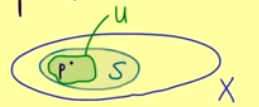
\includegraphics[width=\textwidth]{Figs/interior.png}
        \caption{Interior point}
    \end{subfigure}
    \begin{subfigure}{0.24\textwidth}
        \centering
        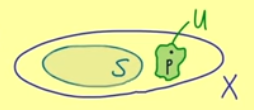
\includegraphics[width=\textwidth]{Figs/exterior.png}
        \caption{Exterior point}
    \end{subfigure}
    \begin{subfigure}{0.24\textwidth}
        \centering
        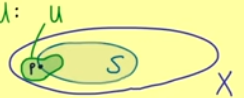
\includegraphics[width=\textwidth]{Figs/boundary.png}
        \caption{Boundary point}
    \end{subfigure}
    \begin{subfigure}{0.24\textwidth}
        \centering
        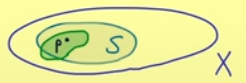
\includegraphics[width=\textwidth]{Figs/accumulation.png}
        \caption{Accumulation point}
    \end{subfigure}
    \caption{Interior, exterior, and boundary points of a set}
\end{figure}


\begin{definition}{\textbf{Interior of a set}} \\
    The interior of a set \( S \), denoted by \( \text{int}(S) \) or \( S^\circ \), is the set of all interior points of \( S \).
    \begin{equation*}
        S^\circ = \{ p \in S : p \text{ is an interior point of } S \}
    \end{equation*}
\end{definition}


\begin{definition}{\textbf{Exterior of a set}} \\
    The exterior of a set \( S \), denoted by \( \text{ext}(S) \), is the set of all exterior points of \( S \).
    \begin{equation*}
        \text{ext}(S) = \{ p \in X : p \text{ is an exterior point of } S \}
    \end{equation*}
\end{definition}

\begin{definition}{\textbf{Boundary of a set}} \\
    The boundary of a set \( S \), denoted by \( \text{bd}(S) \) or \( \partial S \), is the set of all boundary points of \( S \).
    \begin{equation*}
        \partial(S) = \{ p \in X : p \text{ is a boundary point of } S \}
    \end{equation*}
\end{definition}

The boundary of a set \( S \) consists of all points that are either in the interior of \( S \) or in the exterior of \( S \).


\begin{definition}{\textbf{Derived set} (derivative of a set)} \\
    The derived set of a set \( S \), denoted by \( S' \), is the set of all accumulation points of \( S \).
    \begin{equation*}
        S' = \{ p \in X : p \text{ is an accumulation point of } S \}
    \end{equation*}
\end{definition}

\begin{definition}{\textbf{Closure of a set}} \\
    The closure of a set \( S \), denoted by \( \overline{S} \), is the set of all points in \( X \) that are either in \( S \) or are accumulation points of \( S \).
    \begin{equation*}
        \overline{S} = S \cup S'
    \end{equation*}
\end{definition}


\begin{example*}
    X = \( \mathbb{R} \) ,  \( \mathbb{T} = \{ \emptyset, \mathbb{R} \} \cup \{ ( a, \infty ) : a \in \mathbb{R} \} \) is a topology on \( \mathbb{R} \). \\
    S = \( (0, 1) \) is not an open set, and do not have any interior points. \\
    $ X \setminus S = (-\infty, 0] \cup [1, \infty) \Rightarrow  \text{ext}(S) = (1, \infty) \Rightarrow \partial S =  [-\infty, 1)  $.)
    
\end{example*}

\begin{definition}{\textbf{Closed set}} \\
    Let \( (X, \mathcal{T}) \) be a topological space. A set \( S \subseteq X \) is closed if any of the following equivalent conditions hold:
    \begin{itemize}
        \item A set \( S \) is closed if it contains all of its boundary points.
        \item A set \( S \) is closed if its complement \( X \setminus S \) is open.
        \item A set \( S \) is closed if it is equal to its closure \( \overline{S} \).
    \end{itemize}
\end{definition}

% * * * * * * * * * * * * * * * * * * * * * * * *
% * * * * * * * * * * * * * * * * * * * * * * * *
% * * * * * * * * * * * * * * * * * * * * * * * *
% * * * * * * * * * * * * * * * * * * * * * * * *
% * * * * * * * * * * * * * * * * * * * * * * * *
% * * * * * * * * * * * * * * * * * * * * * * * *
% * * * * * * * * * * * * * * * * * * * * * * * *

\section{Hausdorff space}

\begin{definition}{\textbf{Open neighbothood of a point}} \\
    An open neighborhood of a point \( a \) in a topological space \( (X, \mathcal{T}) \) is an open set containing \( a \).
\end{definition}

\begin{definition}{ \textbf{Convergence of a sequence} } \\
    A sequence \( (x_n) \) in a topological space \( (X, \mathcal{T}) \) is said to converge to a limit \( a \in X \) 
    if for every open neighborhood \( U \) of \( a \), there exists a positive integer \( N \) such that for all positive integers \( n \geq N \), \( x_n \in U \).
\end{definition}

Note that there can be multiple limits of a sequence in a topological space, and the limit need not be unique.

\begin{example*}
    X = \( \mathbb{R} \) ,  \( \mathbb{T} = \{ \emptyset, \mathbb{R} \} \cup \{ ( a, \infty ) : a \in \mathbb{R} \} \) is a topology on \( \mathbb{R} \). \\
    \( (a_n)_{n \in \mathbb{N}} = (\frac{1}{n})_{n \in \mathbb{N}} \) converges to 0, but also to any \( a \in (0, \infty) \).
    \begin{itemize}
        \item It converges to 0 - every open neighborhood of 0 looks like \( (a, \infty) \) for some \( a < 0 \) so \( \frac{1}{n} \in (a, \infty) \).
        \item It converges to -1 - every open neighborhood of -1 looks like \( (a, \infty) \) for some \( a < -1 \) so \( \frac{1}{n} \in (a, \infty) \).
        \item The same argument can be made for any \( a \in (-\infty, 0] \).
    \end{itemize}
\end{example*}

\begin{definition}{\textbf{Hausdorff Space}} \\
    A topological space \( (X, \mathcal{T}) \) is a Hausdorff space if for every pair of distinct points \( x, y \in X \), there exist open sets \( U \) and \( V \) such that \( x \in U \), \( y \in V \), and \( U \cap V = \emptyset \).
\end{definition}

\begin{figure}[H]
    \centering
    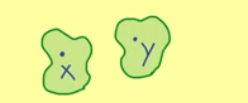
\includegraphics[width=0.3\textwidth]{Figs/hausdorff_space.png}
    \caption{Hausdorff space}
\end{figure}

In a Hausdorff space, every pair of distinct points can be separated by disjoint open sets.

% * * * * * * * * * * * * * * * * * * * * * * * *
% * * * * * * * * * * * * * * * * * * * * * * * *
% * * * * * * * * * * * * * * * * * * * * * * * *
% * * * * * * * * * * * * * * * * * * * * * * * *
% * * * * * * * * * * * * * * * * * * * * * * * *
% * * * * * * * * * * * * * * * * * * * * * * * *
% * * * * * * * * * * * * * * * * * * * * * * * *


\section{Quotient space}

\begin{definition}{\textbf{Projective space}} \\
    The projective space \( \mathbf{P}^n (\mathbb{R}) \) is the set of all lines passing through the origin in \( \mathbb{R}^{n+1} \).
    It can be thought of as the space of all one-dimensional subspaces of \( \mathbb{R}^{n+1} \).
\end{definition}

\begin{figure}[H]
    \centering
    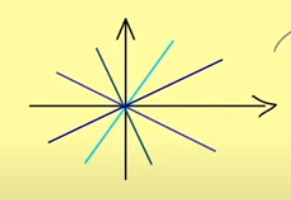
\includegraphics[width=0.3\textwidth]{Figs/projective_space_2d.png}
    \caption{The projective space \( \mathbf{P}^1 \) - all the lines passing through the origin in \( \mathbb{R}^2 \) }
\end{figure}

The directions define a set, and we want to create a topological space for this set.

\begin{definition}{\textbf{Equivalence relation}} \\
    An equivalence relation on a set \( X \) is a relation \( \sim \) that satisfies the following properties for all \( x, y, z \in X \):
    \begin{enumerate}
        \item Reflexivity: \( x \sim x \)
        \item Symmetry: \( x \sim y \) implies \( y \sim x \)
        \item Transitivity: \( x \sim y \) and \( y \sim z \) implies \( x \sim z \)
    \end{enumerate}
\end{definition}

\begin{definition}{\textbf{Equivalence class}} \\
    Let \( X \) be a set and \( \sim \) be an equivalence relation on \( X \). \\
    The equivalence class of \( x \) with respect to \( \sim \) is
    \begin{equation*}
        [x]_\sim = \{ y \in X : y \sim x \}
    \end{equation*}
\end{definition}

\begin{definition}{\textbf{Quotient set}} \\
    Let \( X \) be a set and \( \sim \) be an equivalence relation on \( X \). \\
    The quotient set \( X / \sim \) is defined as 
    \begin{equation*}
        X/\sim \quad = \{ [x]_\sim : x \in X \}
    \end{equation*}
\end{definition}

\begin{definition}{\textbf{Quotient map (Canonical projection)}} \\
    Let \( X \) be a set and \( \sim \) be an equivalence relation on \( X \). \\
    The canonical projection is a function:
    \begin{equation*}
        q: X \to X/\sim \quad \text{such that} \quad q(x) = [x]_\sim
    \end{equation*}
\end{definition}

\begin{definition}{\textbf{Quotient Topology}} \\
    Let \( X , \mathcal{T} \) be a topological space, \( \sim \) be an equivalence relation on \( X \) and \( q: X \to X/\sim \) be the canonical projection. \\
    The quotient topology \( \hat{\mathcal{T}} \) on \( X/\sim \) is defined as
    \begin{equation*}
        \hat{\mathcal{T}} = \{ U \subseteq X/\sim \quad : q^{-1}(U) \in \mathcal{T} \}
    \end{equation*}
\end{definition}

\begin{figure}[H]
    \centering
    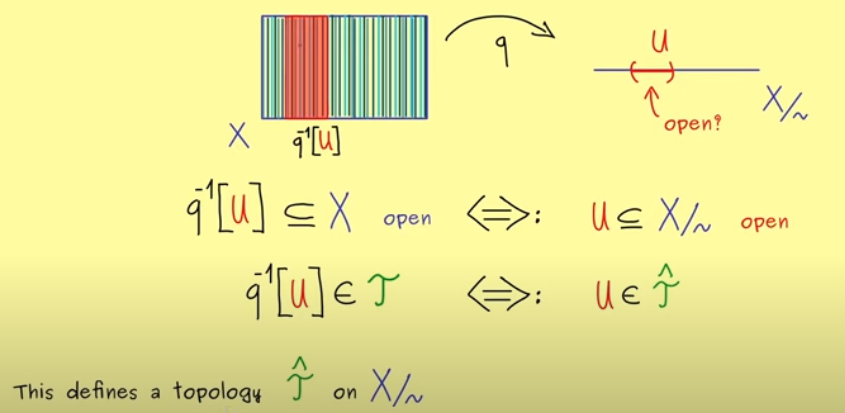
\includegraphics[width=0.8\textwidth]{Figs/quotient_topology.png}
    \caption{Quotient Topology}
\end{figure}

\begin{example*} A classic example of a quotient space is the \textbf{mobius strip}, which is constructed by taking a rectangular strip of paper, 
    giving one end a half-twist, and then gluing the two ends together. The mobius strip is a non-orientable surface, 
    meaning that it does not have a consistent notion of "left" and "right" across the entire surface. 
    The mobius strip is a quotient space of a square, where the opposite edges of the square are identified in a specific way.
    Formally, 
    \begin{align*}
        X = [0, 1] \times (-1, 1) \quad \text{and} \quad &\sim \text{ is the equivalence relation that identifies the points} \\
        (0, y) &\sim (1, -y) \quad \text{for all} \quad y \in (-1, 1).
    \end{align*}
\end{example*}

\begin{figure}[H]
    \centering
    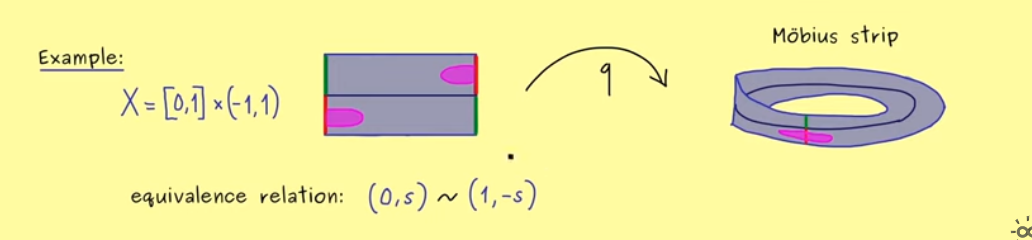
\includegraphics[width=0.8\textwidth]{Figs/mobius_strip.png}
    \caption{Mobius Strip}
\end{figure}

% * * * * * * * * * * * * * * * * * * * * * * * *
% * * * * * * * * * * * * * * * * * * * * * * * *
% * * * * * * * * * * * * * * * * * * * * * * * *
% * * * * * * * * * * * * * * * * * * * * * * * *
% * * * * * * * * * * * * * * * * * * * * * * * *
% * * * * * * * * * * * * * * * * * * * * * * * *
% * * * * * * * * * * * * * * * * * * * * * * * *


\section{Projective Space}

So far we have seen the transition from topological space to quotient space:
\begin{equation*}
    (X, \mathcal{T}) \to (X/\sim, \hat{\mathcal{T}})
\end{equation*}

Recall that the projective space \( \mathbf{P}^n (\mathbb{R}) \) is the set of all lines passing through the origin in \( \mathbb{R}^{n+1} \).

\begin{definition}{\textbf{Sphere}} \\
    The sphere \( S^n \) is the set of all points in \( \mathbb{R}^{n+1} \) that are at a fixed distance of 1 from the origin.
    \begin{equation*}
        S^n = \{ x \in \mathbb{R}^{n+1} : \|x\|_2 = 1 \}
    \end{equation*}
\end{definition}

\begin{definition}{\textbf{The Projective Space as quotient space}} \\
    The projective space \( \mathbf{P}^n (\mathbb{R}) \) can be constructed as a quotient space of the sphere \( S^n \) by identifying antipodal points.
    \begin{equation*}
        \mathbf{P}^n (\mathbb{R}) = S^n / \sim
    \end{equation*}
    where the equivalence relation \( \sim \) is defined as
    \begin{equation*}
        x \sim y \quad \text{if} \quad x = y \quad \text{or} \quad x = -y
    \end{equation*}
\end{definition}

\begin{figure}[H]
    \centering
    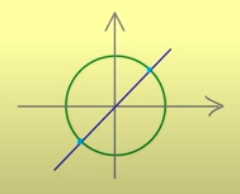
\includegraphics[width=0.3\textwidth]{Figs/projective_space.png}
    \caption{Projective Space as a quotient space}
\end{figure}

The sphere \( S^n \) is a hausdorff space, and the projective space \( \mathbf{P}^n (\mathbb{R}) \) is also a hausdorff space.
But in general, the quotient space of a hausdorff space is not necessarily a hausdorff space.
Take \( [x]_\sim, [y]_\sim \in \mathbf{P}^n (\mathbb{R}) \) such that \( [x]_\sim \neq [y]_\sim \Rightarrow x \neq y \) and \( x \neq -y \) .

\begin{figure}[H]
    \begin{subfigure}{\textwidth}
        \centering
        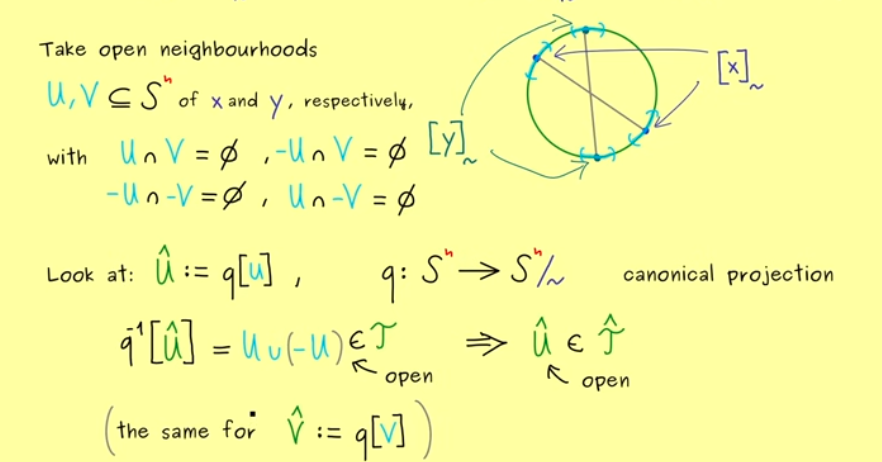
\includegraphics[width=\textwidth]{Figs/projective_space_is_hausdorff.png}
    \end{subfigure}
    \begin{subfigure}{\textwidth}
        \centering
        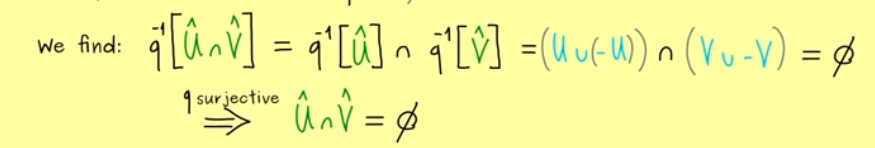
\includegraphics[width=\textwidth]{Figs/projective_space_is_hausdorff2.png}
    \end{subfigure}
    \caption{Projective Space as a hausdorff space}
\end{figure}

% * * * * * * * * * * * * * * * * * * * * * * * *
% * * * * * * * * * * * * * * * * * * * * * * * *
% * * * * * * * * * * * * * * * * * * * * * * * *
% * * * * * * * * * * * * * * * * * * * * * * * *
% * * * * * * * * * * * * * * * * * * * * * * * *
% * * * * * * * * * * * * * * * * * * * * * * * *
% * * * * * * * * * * * * * * * * * * * * * * * *

\section{First Countable Space}

\begin{definition}{\textbf{First Countable Space}} \\
    A topological space \( (X , \mathcal{T}) \) is said to be \emph{first countable} if at every point \( x \) in \( X \), 
    there exists a countable basis for the neighborhoods of \( x \). That is: \\ 
    \begin{align*}
        &\forall x \in X, \quad \exists \{ U_i \}_{i=1}^{\infty} \quad \text{such that} \quad \forall i \in \mathbb{N} \quad x \in U_i \\
        &\text{and} \quad \forall V \in \mathcal{T} \quad \text{such that} \quad x \in V , \quad \exists i \quad \text{such that} \quad U_i \subseteq V
    \end{align*}
    The countable set of open sets \( \{ U_i \}_{i=1}^{\infty} \) is called a \textbf{local basis} at \( x \).
\end{definition}

\begin{examples*} of first countable spaces:
    \begin{itemize}
        \item \textbf{Metric Spaces}: Every metric space is first countable. 
        The local basis at any point \( x \) in a metric space can be chosen as the collection of open balls centered 
        at \( x \) with radii \( 1/n \), where \( n \) is a positive integer.

        \item \textbf{Subspaces of Metric Spaces}: Any subspace of a metric space inherits the first countability. 
        If \( Y \) is a subspace of a metric space \( X \), then the local bases in \( Y \) can be constructed using 
        the intersections of open balls in \( X \) with \( Y \).

        \item \textbf{Euclidean Spaces \( \mathbb{R}^n \)}: The Euclidean space with its standard topology, 
        which is generated by the open balls, is first countable.

        \item \textbf{The Space of Rational Numbers \( \mathbb{Q} \)}: As a subspace of the real line \( \mathbb{R} \), 
        which is a metric space, the space of rational numbers \( \mathbb{Q} \) is first countable.
    \end{itemize}
\end{examples*}

\section{Second Countable Space}

\begin{definition}{\textbf{Basis}} \\
    A basis for a topological space \( (X, \mathcal{T}) \) is a collection \( \mathcal{B} \subseteq \mathcal{T} \) of open sets 
    such that every open set in \( \mathcal{T} \) can be written as a union of sets in \( \mathcal{B} \).
\end{definition}

\begin{examples*} of basis:
    \begin{itemize}
        \item \( \mathcal{B} = \mathcal{T} \) is a basis for \( \mathcal{T} \).
        \item If \( \mathcal{T} \) is discrete, then \( \mathcal{B} = \{ \{ x \} : x \in X \} \) is a basis for \( \mathcal{T} \).
        \item Let \( (X, \mathcal{T}) \) be a topological space induced by a metric space \( (X, d) \). \\
            Then \( \mathcal{B} = \{ B_\varepsilon(x) : x \in X, \varepsilon > 0 \} \) is a basis for \( \mathcal{T} \).
        \item \( \mathbb{R}^n \) with the standard topology (defined by the Euclidean metric) has a basis of open balls.
            Then \( \mathcal{B} = \{ B_{\varepsilon}(x) : x \in \mathbb{Q}^n, \varepsilon \in \mathbb{Q}, \varepsilon > 0 \} \) is a basis for \( \mathcal{T} \).
            Eventhought the space is uncountable, the basis has a countable number of elements.
    \end{itemize}
\end{examples*}

\begin{definition}{\textbf{Second Countable Space}} \\
    A topological space \( (X, \mathcal{T}) \) is second countable if there exists a countable basis for \( \mathcal{T} \).
\end{definition}


\begin{examples*} of second countable spaces:
    \begin{itemize}
        \item Any finite or countable discrete space.
        \item The real line \( \mathbb{R} \) with the standard topology.
        \item The Euclidean space \( \mathbb{R}^n \) with the standard topology.
        \item The space of continuous functions \( C([0, 1]) \) with the topology of uniform convergence.
    \end{itemize}
\end{examples*}

\begin{examples*} of spaces that are not second countable:
    \begin{itemize}
        \item Consider an uncountable set (like \( \mathbb{R} \)) with the discrete metric (the distance between each pair of distinct
         points is 1, and the distance between a point and itself is 0). 
         In this metric space, every singleton set is open, therefore to have a base for the topology, we need to include every singleton,
         which is an uncountable number.
    \end{itemize}
    
\end{examples*}

\begin{definition}{\textbf{The space of continuous functions with the topology of uniform convergence}} \\
    Let \( C([0, 1]) \) be the space of continuous functions on the interval \( [0, 1] \). \\
    The topology of uniform convergence on \( C([0, 1]) \) is defined by the basis
    \begin{equation*}
        \mathcal{B} = \{ B_{\varepsilon}(f) : f \in C([0, 1]), \varepsilon > 0 \}
    \end{equation*}
    where \( B_{\varepsilon}(f) = \{ g \in C([0, 1]) : \| f - g \|_{\infty} < \varepsilon \} \).
\end{definition}

\begin{figure}[H]
    \centering
    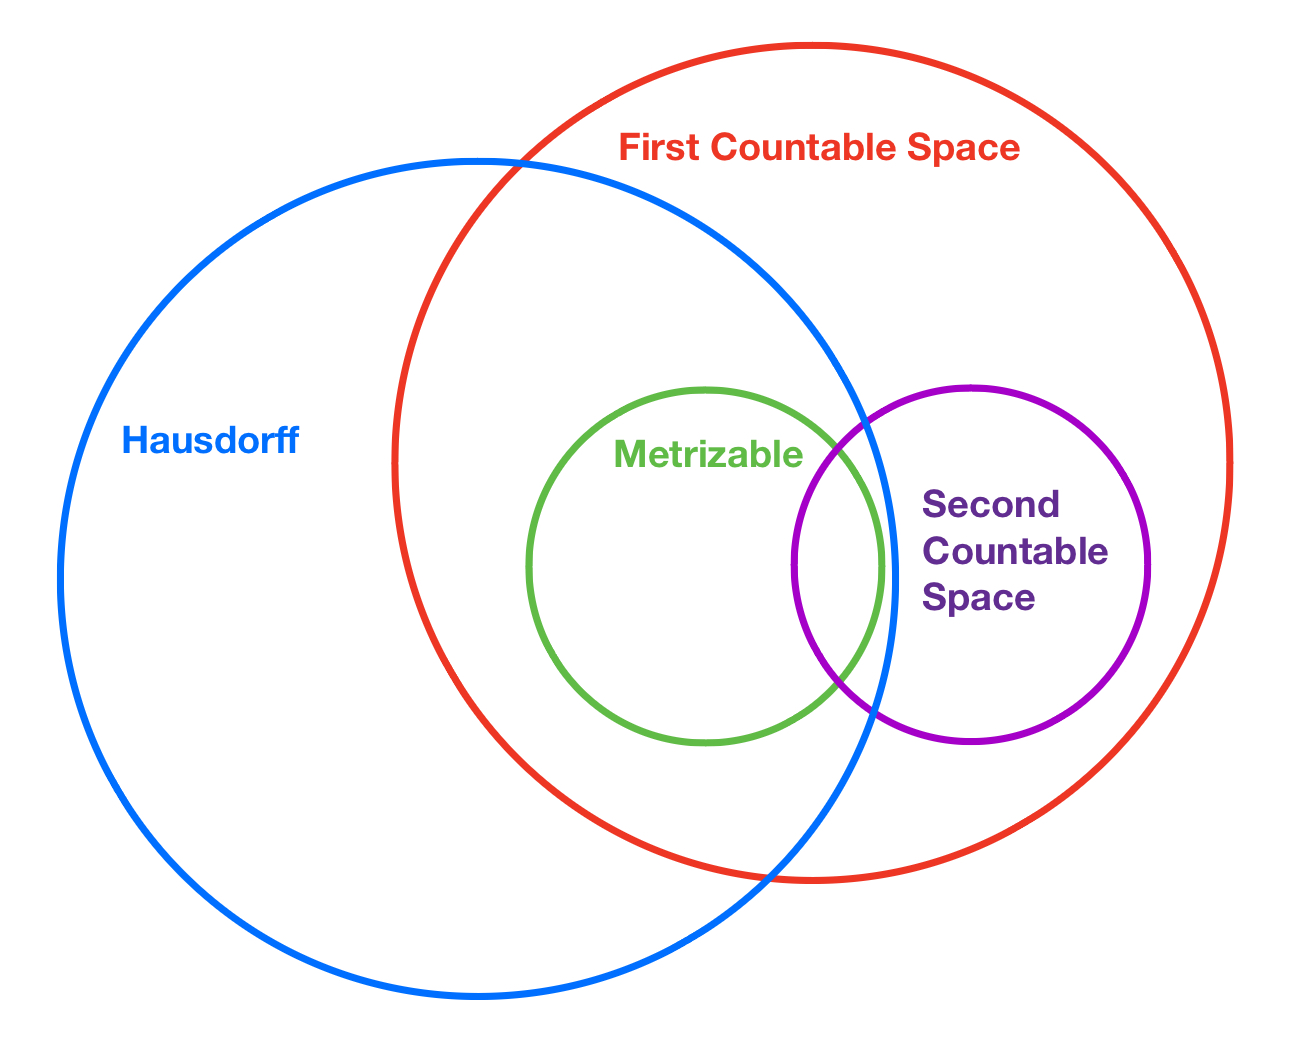
\includegraphics[width=0.5\textwidth]{Figs/topological_spaces_diagram.jpeg}
    \caption{Venn diagram of topological spaces - Metrizable, Hausdorff, First Countable, Second Countable}
\end{figure}


% * * * * * * * * * * * * * * * * * * * * * * * *
% * * * * * * * * * * * * * * * * * * * * * * * *
% * * * * * * * * * * * * * * * * * * * * * * * *
% * * * * * * * * * * * * * * * * * * * * * * * *
% * * * * * * * * * * * * * * * * * * * * * * * *
% * * * * * * * * * * * * * * * * * * * * * * * *
% * * * * * * * * * * * * * * * * * * * * * * * *

\section{Continuity}

Recall the definition of continuity of a function in $R^n$:
\begin{definition*}{\textbf{Continuity of a function}} \\
    A function \( f: \mathbb{R}^n \to \mathbb{R} \) is continuous at a point \( x \in \mathbb{R}^n \) 
    if for every \( \varepsilon > 0 \), there exists \( \delta > 0 \) such that for all \( y \in \mathbb{R}^n \) with
     \( \| x - y \|_2 < \delta \), we have \( \| f(x) - f(y) \|_2 < \varepsilon \).
\end{definition*}

or equivalently, in term of sequences:
\begin{definition*}{\textbf{Continuity of a function (sequence definition)}} \\
    A function \( f: \mathbb{R}^n \to \mathbb{R} \) is continuous at a point \( x \in \mathbb{R}^n \) 
    if for every sequence \( (x_k) \) in \( \mathbb{R}^n \) such that \( x_k \to x \), we have \( f(x_k) \to f(x) \).
\end{definition*}

Now, we extend the definition of continuity to topological spaces.

\begin{definition}{\textbf{Continuity of a function at a point (topological space)}} \\
    Let \( (X, \mathcal{T}_X) \) and \( (Y, \mathcal{T}_Y) \) be topological spaces. \\
    A function \( f: X \to Y \) is continuous at a point \( x \in X \) if for every neighborhood \( V \) of \( f(x) \) in \( Y \),
    there exists a neighborhood \( U \) of \( x \) in \( X \) such that \( f(U) \subseteq V \).
\end{definition}

\begin{figure}[H]
    \centering
    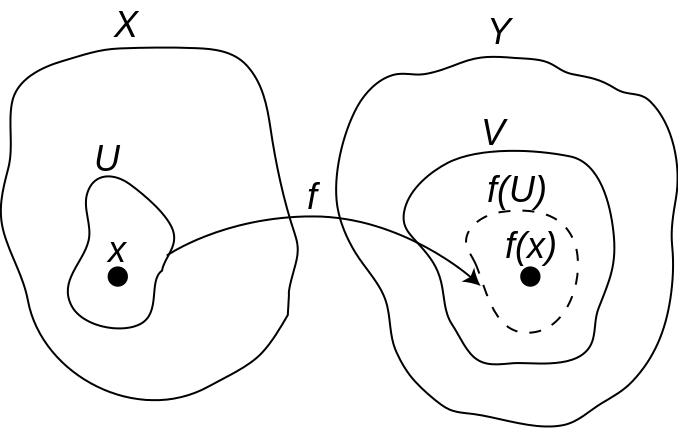
\includegraphics[width=0.4\textwidth]{Figs/continuity_topology.png}
    \caption{Continuity of a function at a point} 
\end{figure}


\begin{definition}{\textbf{Continuity of a function (topological space)}} \\
    Let \( (X, \mathcal{T}_X) \) and \( (Y, \mathcal{T}_Y) \) be topological spaces. \\
    A function \( f: X \to Y \) is continuous if for every open set \( U \in \mathcal{T}_Y \), \( f^{-1}(U) \in \mathcal{T}_X \) \\
    (the preimage of an open set is open).
\end{definition}

\begin{figure}[H]
    \centering
    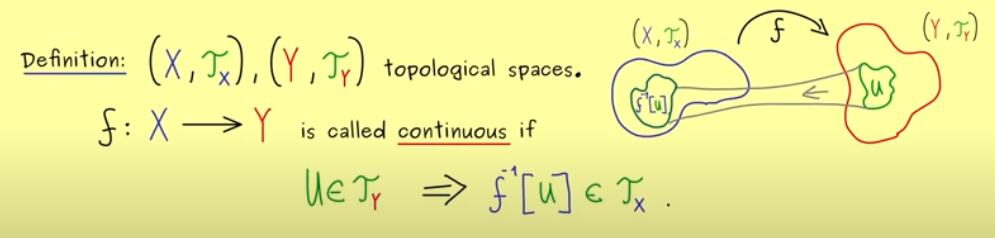
\includegraphics[width=\textwidth]{Figs/continuity.png}
    \caption{Continuity of a function}    
\end{figure}

In term of sequences:

\begin{definition}{\textbf{Sequentially continuous function (topological space)}} \\
    Let \( (X, \mathcal{T}_X) \) and \( (Y, \mathcal{T}_Y) \) be topological spaces. \\
    A function \( f: X \to Y \) is sequentially continuous if for every \( x \in X \) and every sequence 
    \( (x_n)_{n \in \mathbb{N}} \subseteq X \) such that \( x_n \to x \), \( (f(x_n))_{n \in \mathbb{N}} \subseteq Y \) convergent 
    with \( (f(x_n))_{n \in \mathbb{N}} \to f(x) \).
\end{definition}

\begin{figure}[H]
    \centering
    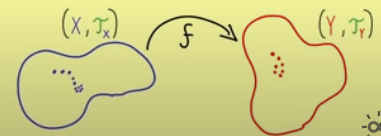
\includegraphics[width=0.4\textwidth]{Figs/sequentially_continues_function.png}
    \caption{Sequentially continuous function}
\end{figure}

\begin{theorem}{\textbf{Continuity vs Sequential Continuity}} \\
    Let \( (X, \mathcal{T}_X) \) and \( (Y, \mathcal{T}_Y) \) be topological spaces and \( f: X \to Y \) be a function. \\
    \begin{align*}
        \text{f is continuous} &\Rightarrow \text{f is sequentially continuous} \\
        \text{f is continuous} &\nLeftarrow \text{f is sequentially continuous}
    \end{align*}
\end{theorem}

\begin{theorem}{\textbf{Continuity vs Sequential Continuity in First Countable Spaces}} \\
    Let \( (X, \mathcal{T}_X) \) and \( (Y, \mathcal{T}_Y) \) be First Countable spaces and \( f: X \to Y \) be a function. Then 
    \begin{align*}
        \text{f is continuous} &\Leftrightarrow \text{f is sequentially continuous}
    \end{align*}
\end{theorem}

\begin{examples*} of continuous maps
    \begin{itemize}
        \item The indiscrete topology on \( X \) and \( Y \) - every function is continuous. \\
            e.g., \( \forall f: X \to Y \) , \( \mathcal{T}_X = \{ \emptyset, X \} \) and \( \mathcal{T}_Y = \{ \emptyset, Y \} \), 
            then \( f \) is continuous since the preimage of any open set in \( Y \) is either \( \emptyset \) or \( X \).

        \item The discrete topology on \( X \) and \( Y \) - every function is continuous. \\
            e.g., \( \forall f: X \to Y \) , \( \mathcal{T}_X = P(X) \) and \( \mathcal{T}_Y = P(Y) \), 
            then \( f \) is continuous since the preimage of any open set in \( Y \) must be a subset of \( X \).

        \item The quotient map \( q: X \to X/\sim \) is continuous. \\
            Let \( (X, \mathcal{T}) \) be a topological space and \( \sim \) be an equivalence relation on \( X \). \\
            Then the quotient map \( q: X \to X/\sim \) is continuous.
            \begin{proof}
                Let \( U \in \mathcal{T}_{X/\sim} \) be an open set in \( X/\sim \). \\
                Then \( q^{-1}(U) \in \mathcal{T}_X \) is an open set in \( X \) by definition of the quotient topology. 
                The same argument holds for the other direction.
            \end{proof}
    \end{itemize}
\end{examples*}

\begin{definition}{\textbf{Homeomorphism} (NOT homomorphism)}\label{def:homeomorphism} \\ 
    A function \( f: X \to Y \) between topological spaces \( (X, \mathcal{T}_X) \) and \( (Y, \mathcal{T}_Y) \) is a homeomorphism if
    \begin{enumerate}
        \item \( f \) is bijective (both injective and surjective - one-to-one and onto).
        \item \( f : X \to Y \) is continuous.
        \item \( f^{-1} : Y \to X \) is continuous.
    \end{enumerate}
\end{definition}

Not all continuous functions are homeomorphisms.
For example, a quotient map is continuous but not necessarily a homeomorphism, if more than one point is mapped 
to the same equivalence class.


% * * * * * * * * * * * * * * * * * * * * * * * *
% * * * * * * * * * * * * * * * * * * * * * * * *
% * * * * * * * * * * * * * * * * * * * * * * * *
% * * * * * * * * * * * * * * * * * * * * * * * *
% * * * * * * * * * * * * * * * * * * * * * * * *
% * * * * * * * * * * * * * * * * * * * * * * * *
% * * * * * * * * * * * * * * * * * * * * * * * *

\section{Compactness}

We know that any closed and bounded subset of \( \mathbb{R} \) is compact, for example, the closed interval \( [a, b] \in \mathbb{R} \) is compact.

\begin{definition}{\textbf{Compact set}} \\
    Let \( (X, \mathcal{T}) \) be a topological space, and \( A \subseteq X \). \\
    \( A \) is called compact if for every open cover \( \{ U_i \}_{i \in I} \) of \( A \), there exists a finite subcover of \( A \).
    \begin{equation*}
        A \subseteq \bigcup_{i \in I} U_i \quad \Rightarrow \quad A \subseteq \bigcup_{i \in I_0} U_i \quad \text{for some finite} \quad I_0 \subseteq I
    \end{equation*}
    
\end{definition}

\begin{figure}[H]
    \centering
    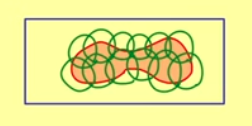
\includegraphics[width=0.3\textwidth]{Figs/compact_set.png}
    \caption{Compact set - every open cover has a finite subcover}
\end{figure}

We are already familiar with the Heine-Borel theorem for compact sets in \( \mathbb{R}^n \) with the standard topology.
\begin {theorem}{\textbf{Heine-Borel Theorem}} \\
    A subset \( A \subseteq \mathbb{R}^n \) is compact \( \Leftrightarrow A \) is closed and bounded.
\end{theorem}

We don't have this theorem for general topological spaces, simply because the term "bounded" is not defined in a general topological spaces.
If we had a metric we could define boundedness in terms of the metric, but even then the Heine-Borel theorem would not hold in general.

\begin{theorem}{\textbf{Compactness in hausdorff spaces}} \\
    Let \( (X, \mathcal{T}) \) be a hausdorff space and \( A \subseteq X \). \\ 
    If \( A \) is compact, then \( A \) is closed.
\end{theorem}

\begin{proof}
    Let \( A \) be a compact set in a hausdorff space \( X \). \\
    We want to show that \( A \) is closed. \\
    Let \( b \in X \setminus A \). 
    For every \( a \in A \), since \( X \) is hausdorff, there exist open sets \( U_a \) and \( V_a \) such that \( a \in U_a \), \( b \in V_a \), and \( U_a \cap V_a = \emptyset \). \\
    Then \( \{ U_a \}_{a \in A} \) is an open cover of \( A \). \\
    Since \( A \) is compact, there exists a finite subcover \( \{ U_{a_1}, U_{a_2}, \ldots, U_{a_n} \} \) of \( A \). \\
    Let \( V = \bigcap_{i=1}^n V_{a_i} \). \\
    Then \( V \) is an open set containing \( b \) and \( V \cap A = \emptyset \), which implies that \( b \) is an interior point of \( X \setminus A \). 
    Therefore, \( A \) is closed.
\end{proof}


% * * * * * * * * * * * * * * * * * * * * * * * *
% * * * * * * * * * * * * * * * * * * * * * * * *
% * * * * * * * * * * * * * * * * * * * * * * * *
% * * * * * * * * * * * * * * * * * * * * * * * *
% * * * * * * * * * * * * * * * * * * * * * * * *
% * * * * * * * * * * * * * * * * * * * * * * * *
% * * * * * * * * * * * * * * * * * * * * * * * *


\section{Locally Euclidean Spaces}

\begin{definition}{\textbf{n-dimensional (topological) Manifold}} \\
    A topological space \( (M , \mathcal{T}) \) is called a manifold of dimension \( n \) if it satisfies the following conditions:
    \begin{enumerate}
        \item \( (M , \mathcal{T}) \) is hausdorff space.
        \item \( (M , \mathcal{T}) \) is second countable.
        \item \( (M, \mathcal{T}) \) is locally euclidean of dimension \( n \).
    \end{enumerate}
\end{definition}

\begin{figure}[H]
    \centering
    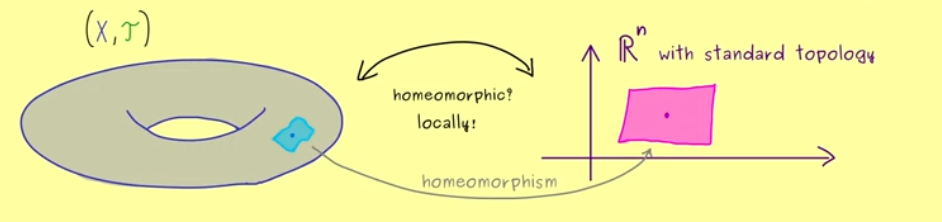
\includegraphics[width=\textwidth]{Figs/locally_euclidean_topological_space.png}
    \caption{Locally Euclidean Topological Space}
\end{figure}

\begin{definition}{\textbf{Locally Euclidean Space}} \\
    A topological space \( (M, \mathcal{T}) \) is locally euclidean of dimension \( n \) if \\ 
    \(\forall x \in M \), there exists an open neighborhood \( U \in \mathcal{T} \) and a homeomorphism \( h: U \to V \) where \( V \) is an open subset of \( \mathbb{R}^n \). \\
    Such an homeomorphism \( h: U \to V \) is called a \textbf{chart} of \( (M , \mathcal{T}) \) at \( x \).
\end{definition}

\begin{figure}[H]
    \centering
    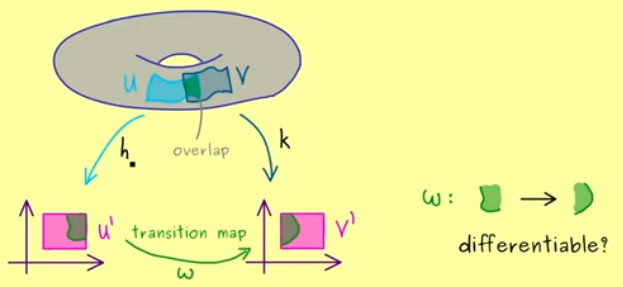
\includegraphics[width=0.7\textwidth]{Figs/chart_of_manifold.png}
    \caption{Charts and Atlases of a Manifold}
\end{figure}



% * * * * * * * * * * * * * * * * * * * * * * * *
% * * * * * * * * * * * * * * * * * * * * * * * *
% * * * * * * * * * * * * * * * * * * * * * * * *
% * * * * * * * * * * * * * * * * * * * * * * * *
% * * * * * * * * * * * * * * * * * * * * * * * *
% * * * * * * * * * * * * * * * * * * * * * * * *
% * * * * * * * * * * * * * * * * * * * * * * * *

\section{Examples of Manifolds}

\begin{definition}{\textbf{Atlas}} \\
    An atlas of a manifold \( M \) is a collection of charts that cover \( M \). \\
    Formally, an atlas \( \mathcal{A} \) of a manifold \( M \) is a collection of charts \( \{ (U_i, h_i) \}_{i \in I} \) such that 
    \begin{equation*}
        M = \bigcup_{i \in I} U_i
    \end{equation*}
\end{definition}

\begin{examples*} of Manifolds
    \begin{itemize}
        \item \( M , \mathcal{T} \) a discrete topological space with countably many points. \\
            Every point in \( M \) is a manifold of dimension 0.

        \item \( M \subseteq \mathbb{R}^n \) with the standard topology, \( (M , \mathcal{T}) \) is a manifold of dimension \( n \). \\
            h is the identity map and M is locally euclidean of dimension n (in fact, it is globally euclidean).

        \item \( S^2 = \{ x \in \mathbb{R}^3 : \| x \|_2 = 1 \} \) is a manifold of dimension 2. \\
            We have seen that \( S^2 \) is a hausdorff space. \\ 
            The atlas of \( S^2 \) consists of two charts: the upper hemisphere and the lower hemisphere. \\
            The upper hemisphere is the set \( U_{3, -} = \{ x \in S^2 : x_3 > 0 \} \) and the lower hemisphere is the set \( U_{3, -}^{'}= \{ x \in S^2 : x_3 < 0 \} \). \\
            The homeomorphism \( h_{3, -}: U_{3, -} \to \mathbb{R}^2 \) is defined as \( h_{3, -}(x_1, x_2, x_3) = (x_1, x_2) \). \\
            The inverse homeomorphism \( h_{3, -}^{-1}: \mathbb{R}^2 \to U_1 \) is defined as \( h_{3, -}^{-1}(x_1, x_2) = (x_1, x_2, \sqrt{1 - x_1^2 - x_2^2}) \). \\
            The same argument holds for the lower hemisphere. \\
            So \( (U_{i, \pm }, h_{i, \pm})_{i \in \{1,2,3\}} \) is an atlas of \( S^2 \).
    \end{itemize}
    
\end{examples*}


% * * * * * * * * * * * * * * * * * * * * * * * *
% * * * * * * * * * * * * * * * * * * * * * * * *
% * * * * * * * * * * * * * * * * * * * * * * * *
% * * * * * * * * * * * * * * * * * * * * * * * *
% * * * * * * * * * * * * * * * * * * * * * * * *
% * * * * * * * * * * * * * * * * * * * * * * * *
% * * * * * * * * * * * * * * * * * * * * * * * *

\section{Projective Space is a Manifold}

As we have seen that the sphere \( S^n = \{ x \in \mathbb{R}^{n+1} : \| x \|_2 = 1 \} \), 
is an n-dimensional manifold with atlas \( (U_{i, \pm}, h_{i, \pm})_{i \in \{1, \dots ,n+1\}} \) 
where \( U_{i, \pm} = \{ x \in \mathbb{R}^{n+1} : \pm x_i > 0 \} \) and \( h_{i, \pm}(x_1, \ldots, x_{n+1}) = (x_1, \ldots, x_{i-1}, x_{i+1}, \ldots, x_{n+1}) \).
We have also seen that the projective space \( \mathbf{P}^n (\mathbb{R}) = S^n / \sim \) with quotient topology and equivalence 
relation \( x \sim y \Leftrightarrow x = y \) or \( x = -y \). \\
We will show that the projective space \( \mathbf{P}^n (\mathbb{R}) \) is a manifold of dimension \( n \).

\medbreak

We will define \( V_i = \{ [x]_\sim \in \mathbf{P}^n : x_i \neq 0 \} \). 
Note that every equivilance class \( [x]_\sim \) contains exactly 2 points from the sphere \( S^n \).
\( q^{-1}[V_i] = U_{i, +} \cup U_{i, -} \) is an open set in the sphere \( S^n \) and \( q: S^n \to \mathbf{P}^n \) is a quotient map,
so \( V_i \) is an open set in the projective space \( \mathbf{P}^n \).

\medbreak

In order to show that \( \mathbf{P}^n (\mathbb{R}) \) is a manifold of dimension \( n \), 
we will present homeomorphisms \( h_i: V_i \to \mathbb{R}^n \) for each \( i \in \{1, \ldots, n+1\} \) such that \( (V_i, h_i) \) is a chart of \( \mathbf{P}^n (\mathbb{R}) \).

\begin{figure}[H]
    \begin{subfigure}{0.5\textwidth}
        \centering
        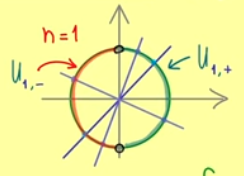
\includegraphics[width=0.5\textwidth]{Figs/projective_space_P1.png}
    \end{subfigure}
    \begin{subfigure}{0.5\textwidth}
        \centering
        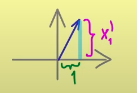
\includegraphics[width=0.5\textwidth]{Figs/projective_space_P1_2.png}
    \end{subfigure}
    \caption{Projective Space of dimension 1 as a quotient space of the circle}
\end{figure}

For n = 1: \\
\( V_1 = \{ [x]_\sim \in \mathbf{P}^1 : x_1 \neq 0 \} \) is an open set in \( \mathbf{P}^1 \). \\
\( q^{-1}[V_1] = U_{1, +} \cup U_{1, -} \) \\
We need homeomorphisms \( h_1: V_1 \to V_1' \) where \( V_1' \) is an open subset of \( \mathbb{R} \). \\
We can define \( h_1: V_1 \to V_1' \) as \( h_1([x]_\sim) = \frac{x_2}{x_1} \) (the slope) for \( x_1 \neq 0 \). \\
The invese homeomorphism \( h_1^{-1}: V_1' \to V_1 \) is defined as \( h_1^{-1}(x1) = [ \binom{1}{x1'} \cdot \frac{1}{\sqrt{1^2 + ({x1'})^2}} ]_\sim \). \\
\( V_2 = \{ [x]_\sim \in \mathbf{P}^1 : x_2 \neq 0 \} \) and we will do the same with the change of coordinates.

\medbreak

For $n \in \mathbb{N}$: \\
\( V_i = \{ [x]_\sim \in \mathbf{P}^n : x_i \neq 0 \} \) is an open set in \( \mathbf{P}^n \). \\
\( q^{-1}[V_i] = U_{i, +} \cup U_{i, -} \) \\
We need homeomorphisms \( h_i: V_i \to V_i' \) where \( V_i' \) is an open subset of \( \mathbb{R}^n \). \\
We can define \( h_i: V_i \to V_i' \) as \( h_i([x]_\sim) = \frac{1}{x_i} (x_1, \ldots, x_{i-1}, x_{i+1}, \ldots, x_{n+1}) \) for \( x_i \neq 0 \). \\
In the inverse we apply 1 to the i-th coordinate and normalize the vector.



% * * * * * * * * * * * * * * * * * * * * * * * *
% * * * * * * * * * * * * * * * * * * * * * * * *
% * * * * * * * * * * * * * * * * * * * * * * * *
% * * * * * * * * * * * * * * * * * * * * * * * *
% * * * * * * * * * * * * * * * * * * * * * * * *
% * * * * * * * * * * * * * * * * * * * * * * * *
% * * * * * * * * * * * * * * * * * * * * * * * *

\section{Smooth structures (differential structures)}

\begin{definition}{\textbf{Transition map}} \\
    Let \( (M, \mathcal{T}) \) be an n-manifold and \( (U, h) \) and \( (V, k) \) be two charts of \( M \). \\
    The transition map \( \omega : h(U \cap V) \to k(U \cap V) \) is called the transition map between the charts \( (U, h) \) and \( (V, k) \).
\end{definition}

Note that the transition map is a transoformation of subset of the $R^n$ space, it does not have to be a linear transformation.

We have seen in definition~\ref{def:C^2_class} that a function \( f: \mathbb{R}^n \to \mathbb{R} \) is of class \( C^2 \) 
if all partial derivatives of \( f \) up to order 2 exist and are continuous. We can extend this definition to manifolds.

\begin{definition}{\textbf{$C^k$-Diffeomorphism (Vector Space)}} \\
    A function \( \omega : \mathbb{R}^n \to \mathbb{R}^n \) $C^k$-diffeomorphism ($ k \in \{0, 1, \cdots\} \cup \{ \infty \} $) if the following conditions hold:
    \begin{enumerate}
        \item \( \omega \) is k times continuously differentiable (partial derivatives up to order k exist and are continuous).
        \item \( \omega \) is bijective (both injective and surjective - one-to-one and onto).
        \item The inverse function \( \omega^{-1} \in C^k \).
    \end{enumerate}
\end{definition}

If $k = \infty$, then \( \omega \) is called a smooth diffeomorphism (or simply a diffeomorphism) - all partial derivatives of \( \omega \) exist and are continuous. \\
If $k = 0$, then \( \omega \) is called a homeomorphism - \( \omega \) is continuous, bijactive, 
and the inverse function \( \omega^{-1} \) is continuous (see definition~\ref{def:homeomorphism}). By the composition of charts, the transition map is a always a homeomorphism.

\begin{definition}{\textbf{$C^k$-smoothly compatible charts}} \\
    Two charts \( (U, h) \) and \( (V, k) \) of a manifold \( M \) are called \( C^k \)-smoothly compatible 
    if the transition map \( \omega: h(U \cap V) \to k(U \cap V) \) is a \( C^k \)-diffeomorphism.
\end{definition}

(If $k = \infty$, then the charts are called smoothly compatible.)

What happens if any two charts of a manifold are $C^k$-smoothly compatible?

\begin{definition}{\textbf{$C^k$-atlas}} \\
    An atlas \( \mathcal{A} = \{ (U_i, h_i) \}_{i \in I} \) of a manifold \( M \) is called a \( C^k \)-atlas 
    if every pair of charts in \( \mathcal{A} \) are \( C^k \)-smoothly compatible.
\end{definition}


\begin{definition}{\textbf{Maximal $C^k$-atlas ($C^k$-smooth structure)}} \\
    A maximal \( C^k \)-atlas of a manifold \( M \) is \( \mathcal{A} \) is:
    \begin{enumerate}
        \item \( \mathcal{A} \) is a \( C^k \)-atlas of \( M \).
        \item For any other \( C^k \)-atlas \( \mathcal{B} \) of \( M \), \( \mathcal{A} \nsubseteq \mathcal{B} \).
    \end{enumerate}
\end{definition}


\begin{definition}{\textbf{n-dimensional $C^k$-smooth manifold}} \\
    A manifold \( M \) is called a \( C^k \)-smooth manifold if: 
    \begin{enumerate}
        \item \( M \) is n-dimensional topological manifold.
        \item There exists a maximal \( C^k \)-atlas of \( M \).
    \end{enumerate}
\end{definition}




% * * * * * * * * * * * * * * * * * * * * * * * *
% * * * * * * * * * * * * * * * * * * * * * * * *
% * * * * * * * * * * * * * * * * * * * * * * * *
% * * * * * * * * * * * * * * * * * * * * * * * *
% * * * * * * * * * * * * * * * * * * * * * * * *
% * * * * * * * * * * * * * * * * * * * * * * * *
% * * * * * * * * * * * * * * * * * * * * * * * *

\section{Examples of smooth manifolds}

\begin{example*}{\textbf{The n-dimensional Euclidean sphere \( S^n \subseteq \mathbb{R}^{n+1} \)}} \\
    We have seen that the sphere \( S^n = \{ x \in \mathbb{R}^{n+1} : \| x \|_2 = 1 \} \), 
    is an n-dimensional manifold with atlas \( (U_{i, \pm}, h_{i, \pm})_{i \in \{1, \dots ,n+1\}} \) 
    where \( U_{i, \pm} = \{ x \in \mathbb{R}^{n+1} : \pm x_i > 0 \} \) and \( h_{i, \pm}(x_1, \ldots, x_{n+1}) = (x_1, \ldots, x_{i-1}, x_{i+1}, \ldots, x_{n+1}) \).
    
    \begin{figure}[H]
        \centering
        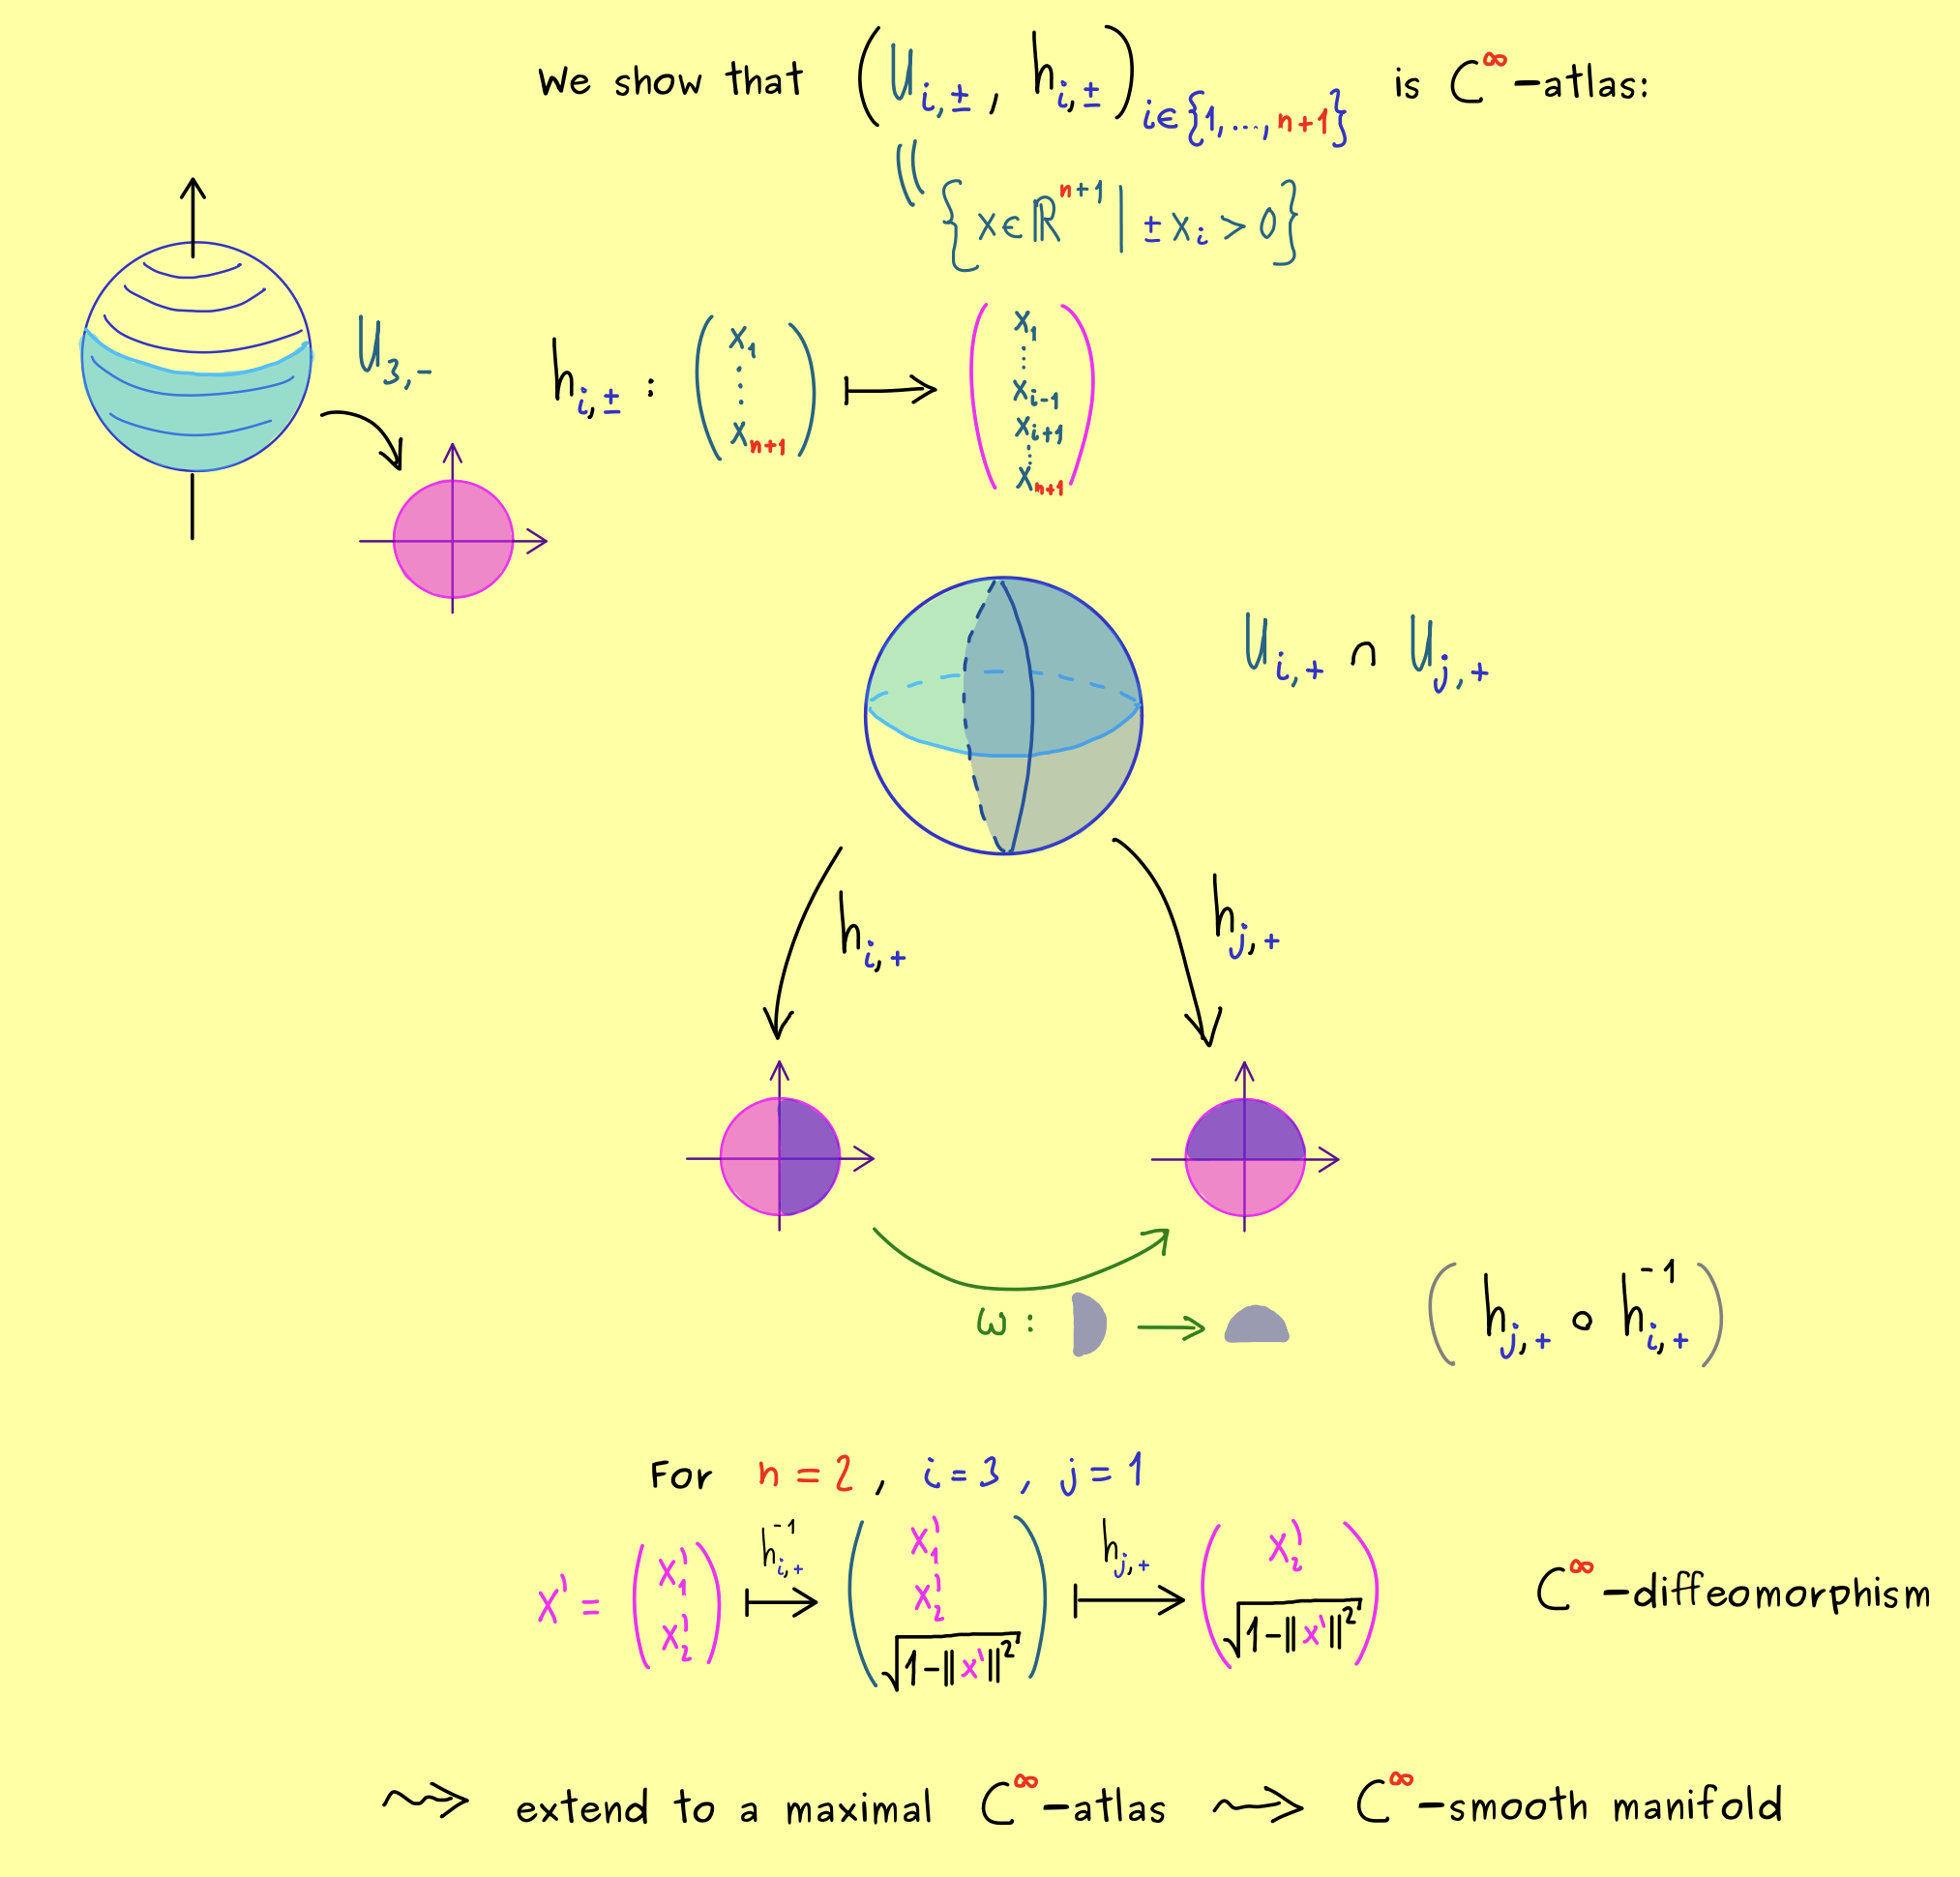
\includegraphics[width=\textwidth]{Figs/sphere_is_C^k_smooth.png}
        \caption{Sphere \( S^n \) is an n-dimensional $C^{\infty}$ smooth manifold}
    \end{figure}
    
\end{example*}

\begin{example*}{\textbf{$\mathbb{R}^n$ is a $C^{\infty}$ smooth manifold}} \\
    The Euclidean space \( \mathbb{R}^n \) is a \( C^{\infty} \) smooth manifold with the atlas \( \{ (\mathbb{R}^n, id) \} \).
    The is the standard smooth structure of \( \mathbb{R}^n \).
\end{example*}

\begin{example*}{\textbf{Consider $f \in C^1$}} \\
    Let \( f: \mathbb{R} \to \mathbb{R} \) be a function of class \( C^1 \). \\
    Let $ G_f = \{ (x, f(x)) \in \mathbb{R}^2 : x \in \mathbb{R} \} $ be the graph of \( f \). \\
    Then \( G_f \) is a \( C^1 \) smooth manifold with one chart: \( h : G_f \to \mathbb{R} \) defined as \( h(x, f(x)) = x \).
\end{example*}

In fact any graph of a function of class \( C^k \) is a \( C^k \) smooth manifold.
We can also observe that $G_f$ is a 1-dimensional $C^1$-smooth manifold that is embedded in another smooth manifold, \( \mathbb{R}^2 \).

% * * * * * * * * * * * * * * * * * * * * * * * *
% * * * * * * * * * * * * * * * * * * * * * * * *
% * * * * * * * * * * * * * * * * * * * * * * * *
% * * * * * * * * * * * * * * * * * * * * * * * *
% * * * * * * * * * * * * * * * * * * * * * * * *
% * * * * * * * * * * * * * * * * * * * * * * * *
% * * * * * * * * * * * * * * * * * * * * * * * *

\section{Submanifolds}

\begin{definition}{\textbf{Submanifold}} \\
    Let \( M \) be a an n-dimensional smooth manifold. 
    \( M_0 \subseteq M \) is called a k-dimensional submanifold of \( M \) if for every \( p \in M_0 \), there exists a chart \( (U, h) \) of \( M \) 
    such that \( h(U \cap M_0) = h(U) \cap (\mathbb{R}^k \times \{ 0 \}^{n-k}) \).
    \((U, h)\) is called a \textbf{submanifold chart} for \( M_0 \).
\end{definition}

Note: \( M_0 \) is also a manifold: 
\( (U, h) submanifold chart \to (\hat{U}, \hat{h}) \) chart, \( \hat{U} = U \cap M_0 \), \( \hat{h} = h|_{\hat{U}} \).

% * * * * * * * * * * * * * * * * * * * * * * * *
% * * * * * * * * * * * * * * * * * * * * * * * *
% * * * * * * * * * * * * * * * * * * * * * * * *
% * * * * * * * * * * * * * * * * * * * * * * * *
% * * * * * * * * * * * * * * * * * * * * * * * *
% * * * * * * * * * * * * * * * * * * * * * * * *
% * * * * * * * * * * * * * * * * * * * * * * * *

\section{Regular value theorem in \( \mathbb{R}^n \)}

\begin{definition}{\textbf{Critical point}} \\
    Let \( f: U \to \mathbb{R}^m \), \( U \subseteq \mathbb{R}^n \) open, \( C^1 \)-function. \\
    A point \( x \in U \) is called a critical point of f if the Jacobian matrix of f at x has rank less than m.
\end{definition}

\begin{definition}{\textbf{Regular value}} \\
    Let \( f: U \to \mathbb{R}^m \), \( U \subseteq \mathbb{R}^n \) open, \( C^1 \)-function. \\
    A point \( y \in f[U] \) is called a regular value of f if for every \( x \in f^{-1}(y) \), x is not a critical point of f.
\end{definition}

\begin{theorem}{\textbf{Regular value theorem in \( \mathbb{R}^n \)}} \\
    Let \( f: U \to \mathbb{R}^m \), \( U \subseteq \mathbb{R}^n \) open, \( C^\infty \)-function. \\
    If c is a regular value of f, then \( f^{-1}[\{c\}] \) is a submanifold of \( \mathbb{R}^n \) of dimension \( n - m \).
\end{theorem}

For example if \( f: \mathbb{R}^n \to \mathbb{R} \), \( f(x_1, \dots, x_n) = x_1^2 + \dots + x_n^2 \), then 0 is a regular value of f. \\
let \( 0 \neq r \in \mathbb{R} \), then r is a regular value of f, for example \( r = 1 \).
Then the sphere \( S^{n-1} \) is a submanifold of \( \mathbb{R}^n \) of dimension \( n - 1 \).


% * * * * * * * * * * * * * * * * * * * * * * * *
% * * * * * * * * * * * * * * * * * * * * * * * *
% * * * * * * * * * * * * * * * * * * * * * * * *
% * * * * * * * * * * * * * * * * * * * * * * * *
% * * * * * * * * * * * * * * * * * * * * * * * *
% * * * * * * * * * * * * * * * * * * * * * * * *
% * * * * * * * * * * * * * * * * * * * * * * * *

\section{Smooth maps}

Until now we have defined smooth manifolds (and \( C^k \)-smooth manifolds). \\
Recall that 
\begin{itemize}
    \item an n-dimensional manifold is a topological space that is locally euclidean of dimension n and hausdorff and second countable.
    \item a smooth manifold is a topological manifold with a maximal \( C^{\infty} \)-atlas.
    \item a \( C^{\infty} \)-atlas is a collection of charts that cover the manifold and the transition 
    maps between any two charts are \( C^{\infty} \)-diffeomorphisms.
    \item \( C^k \)-diffeomorphism is a function that is k times continuously differentiable, bijective, and the inverse function is also \( C^k \).
\end{itemize}

\begin{figure}
    \centering
    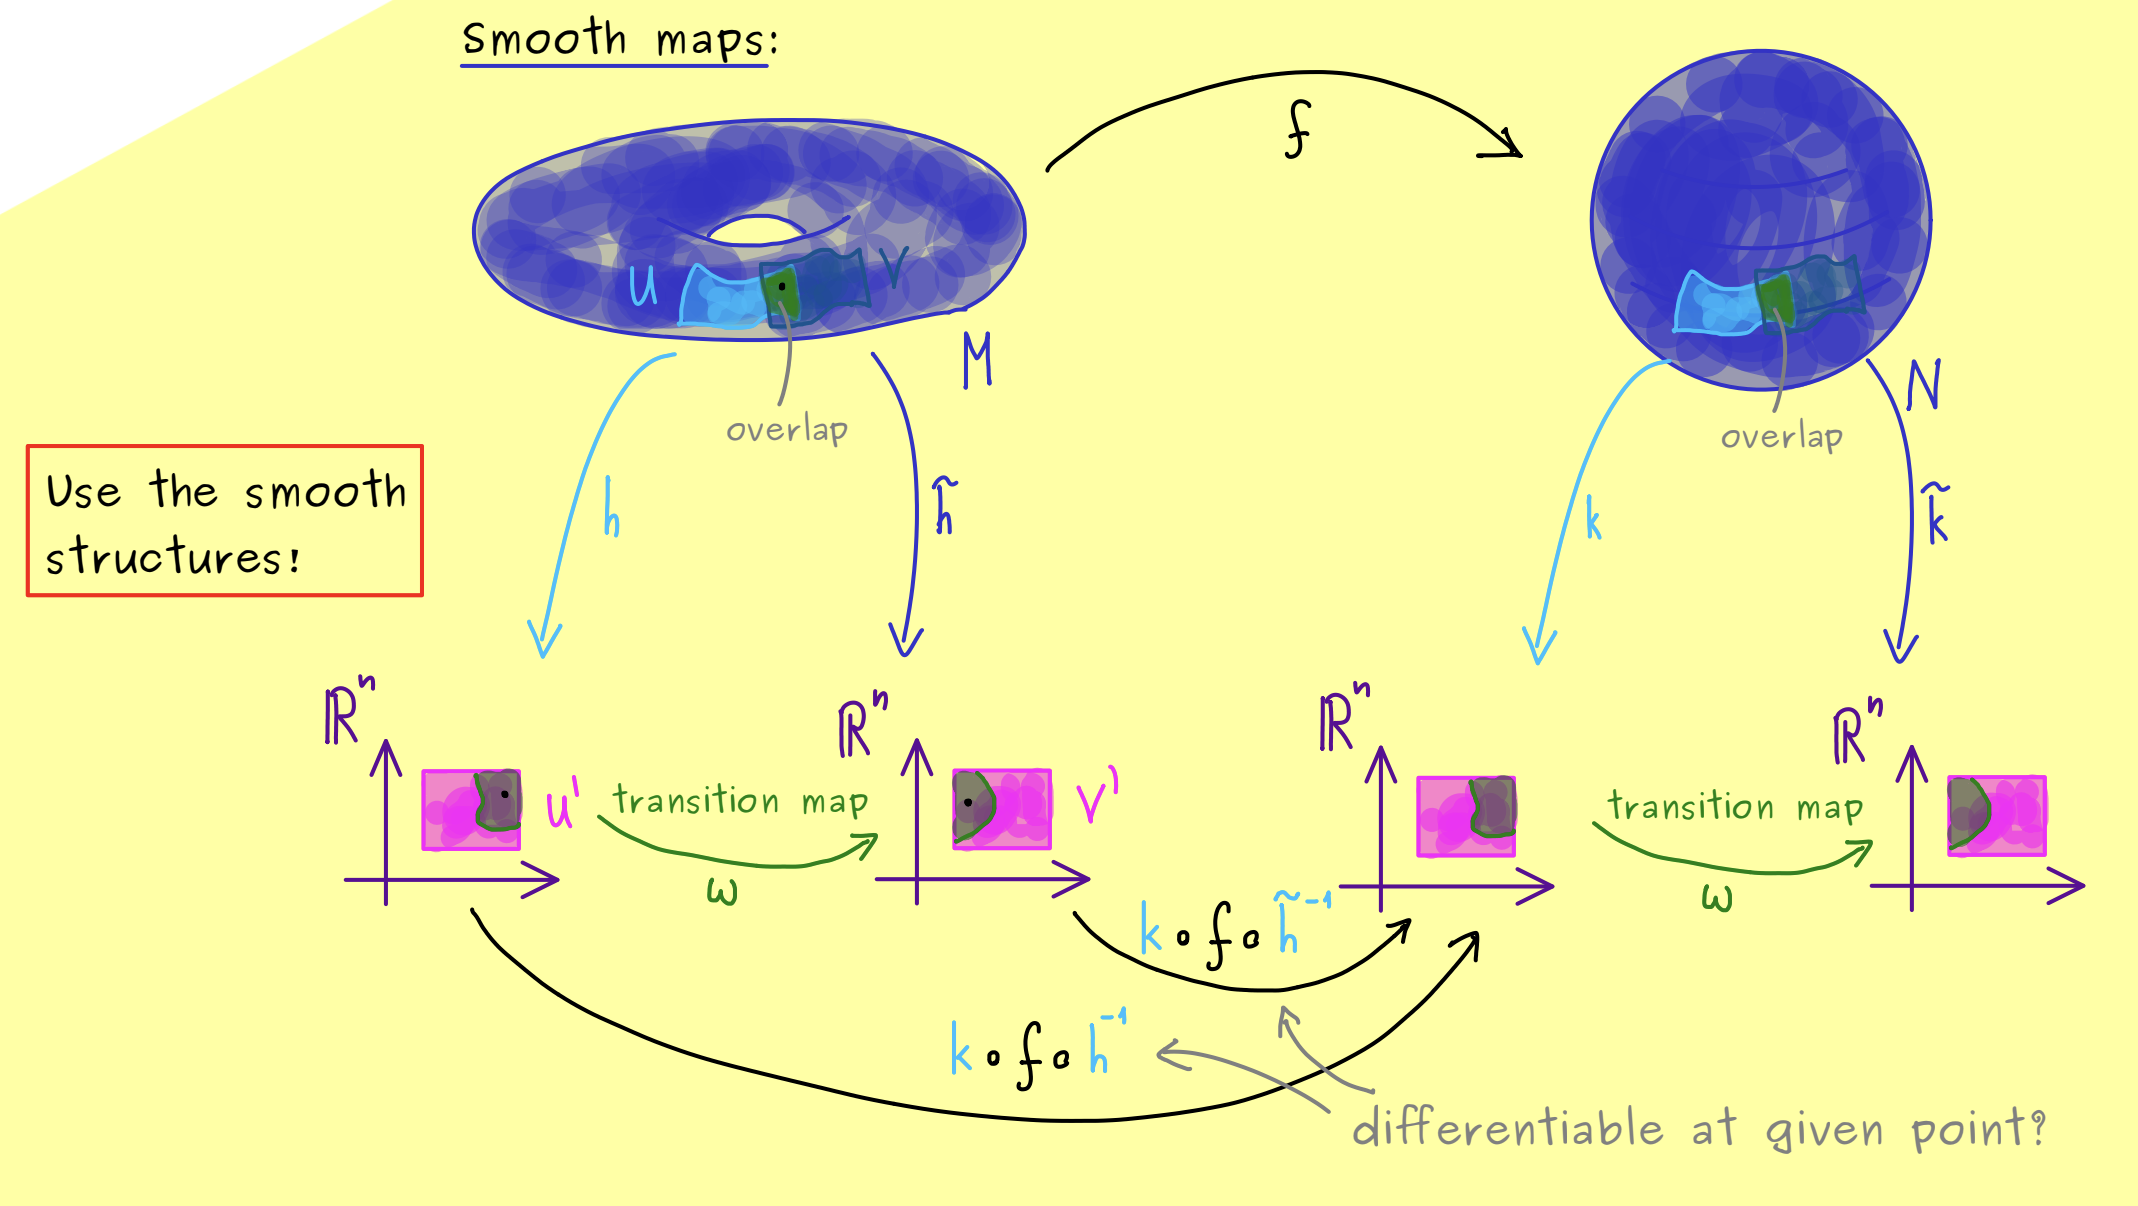
\includegraphics[width=\textwidth]{Figs/smooth_maps.png}
    \caption{Smooth map between two manifolds}
\end{figure}

\begin{definition}{\textbf{k-times differentiable map at a point}} \\
    Let \( f: M \to N \) be a map between two smooth manifolds. \\
    f is called k-times differentiable at a point \( p \in M \) if for every chart \( (U, h) \) of M and every chart \( (W, k) \) of N, 
    with \( p \in U \) and \( f(p) \in V \), the map \( k \circ f \circ h^{-1} \) is k-times differentiable at \( h(p) \).
\end{definition}

\begin{definition}{\textbf{(\(C^\infty\)) Smooth map}} \\
    Let \( f: M \to N \) be a map between two smooth manifolds. \\
    f is called smooth if f is k-times differentiable at every point \( p \in M \) for every \( k \in \mathbb{N} \).
\end{definition}

We often denote the set of smooth maps between two smooth manifolds M and N as \( C^\infty(M, N) \).

% * * * * * * * * * * * * * * * * * * * * * * * *
% * * * * * * * * * * * * * * * * * * * * * * * *
% * * * * * * * * * * * * * * * * * * * * * * * *
% * * * * * * * * * * * * * * * * * * * * * * * *
% * * * * * * * * * * * * * * * * * * * * * * * *
% * * * * * * * * * * * * * * * * * * * * * * * *
% * * * * * * * * * * * * * * * * * * * * * * * *

\section{Examples of smooth maps}

\begin{itemize}
    \item \( S^2 \rightarrow \mathbb{R}^3\) where i is the identity matrix.
    \item the quotient map \( q : S^2 \rightarrow P^2(\mathbb{R}) = S^2 / \sim \)
\end{itemize}


% * * * * * * * * * * * * * * * * * * * * * * * *
% * * * * * * * * * * * * * * * * * * * * * * * *
% * * * * * * * * * * * * * * * * * * * * * * * *
% * * * * * * * * * * * * * * * * * * * * * * * *
% * * * * * * * * * * * * * * * * * * * * * * * *
% * * * * * * * * * * * * * * * * * * * * * * * *
% * * * * * * * * * * * * * * * * * * * * * * * *

\section{Regular value theorem (abstract version)}

\begin{definition}{\textbf{Critical point}} \\
    Let \( f: M \to N \) be a smooth map between two smooth manifolds of dimensions m and n ($m \geq n$). \\
    Let \( p \in M \), \( (U, h) \) a chart of M at p and \((V, k)\) be a chart of N at \(f(p)\). \\
    A point \( p \in M \) is called a critical point of f if 
    \begin{equation*}
        rank(f_p) := rank(J_{k \circ f \circ h^{-1}}(h(p))) < n
    \end{equation*}
\end{definition}
    

\begin{theorem}{\textbf{Regular value theorem (abstract version)}} \\
    Let \( f: M \to N \) be a smooth map between two smooth manifolds of dimensions n and m ($m \geq n$).
    Let \( q \in N \) be a regular value of f. \\
    Then \( f^{-1}[\{q\}] \) is a submanifold of M of dimension \( m - n \).
\end{theorem}

% * * * * * * * * * * * * * * * * * * * * * * * *
% * * * * * * * * * * * * * * * * * * * * * * * *
% * * * * * * * * * * * * * * * * * * * * * * * *
% * * * * * * * * * * * * * * * * * * * * * * * *
% * * * * * * * * * * * * * * * * * * * * * * * *
% * * * * * * * * * * * * * * * * * * * * * * * *
% * * * * * * * * * * * * * * * * * * * * * * * *

\section{Tangent space for submanifolds}

\begin{definition}{\textbf{Local parametrization of a submanifold}} \\
    Let \( M \) be an n-dimensional smooth manifold and \( M_0 \subseteq M \) be a k-dimensional submanifold of \( M \). \\
    Let \( p \in M_0 \) and \( (U, h) \) be a submanifold chart for \( M_0 \) at p, where \( h: U \to U', \quad U' \subseteq \mathbb{R}^k \) is a homeomorphism. \\
    The function \( \varphi : \mathbb{R}^k \cap U' \to M \cap U \) is called a local parametrization of \( M_0 \) at p.
\end{definition}

\begin{example*}The circle
    Let \( S^1 = \{ x \in \mathbb{R}^2 : \| x \|_2 = 1 \} \) be the unit circle in \( \mathbb{R}^2 \). \\
    Let \( M_0 = \{ x \in S^1 : x_1 > 0 \} \) be the right half of the circle. \\
    Let \( p = (1, 0) \in M_0 \) and \( (U, h) \) be a submanifold chart for \( M_0 \) at p, where \( h: U \to U' \) is a homeomorphism. \\
    The function \( \varphi : (0, 2\pi) \to M \cap U \) defined as \( \varphi(t) = (\cos(t), \sin(t)) \) is a local parametrization of \( M_0 \) at p.    
\end{example*}

\begin{definition}{\textbf{The Tangent Space of a submanifold}} \\
    Let \( (M \subseteq \mathbb{R}^n) \) be a k-dimensional submanifold of \( \mathbb{R}^n \). \\
    Let \( p \in M \) and \( \varphi : U' \to U \) be a local parametrization of \( M \) at p. \\
    Let \( \tilde{p} = \varphi^{-1}(p) \). \\
    The tangent space of \( M \) at p is defined as 
    \begin{equation*}
        T_p^{sub} M = d\varphi_{\tilde{p}}[\mathbb{R}^k] = \{ J_{\varphi}(\varphi^{-1}(p)) \cdot v : v \in \mathbb{R}^k \}
    \end{equation*}
\end{definition}

Note thet \( T_p^{sub} M \subseteq \mathbb{R}^n \) is a k-dimensional subspace.
If \( M = \mathbb{R}^n \), then $\phi = \phi^{-1}=id$ , $J_{\phi}(\phi^{-1}(p)) = I$ and $T_p^{sub} \mathbb{R}^n = \mathbb{R}^n$.


% * * * * * * * * * * * * * * * * * * * * * * * *
% * * * * * * * * * * * * * * * * * * * * * * * *
% * * * * * * * * * * * * * * * * * * * * * * * *
% * * * * * * * * * * * * * * * * * * * * * * * *
% * * * * * * * * * * * * * * * * * * * * * * * *
% * * * * * * * * * * * * * * * * * * * * * * * *
% * * * * * * * * * * * * * * * * * * * * * * * *

\section{Tangent curves}

\begin{definition}{\textbf{Smooth curve}} \\
    Let \( M \) be an n-dimensional smooth manifold. \\
    A smooth curve in M is a smooth map \( \gamma: I \to M \) where I is an open interval in \( \mathbb{R} \).
\end{definition}


\begin{definition}{\textbf{Differentiable curve on a manifold \( M \)}} \\
    A differentiable curve on a manifold \( M \) is a function \( \gamma: I \to M \), where \( I \) is an interval in \( \mathbb{R} \). 
    The curve \( \gamma \) is differentiable at a point \( t_0 \in I \) if for every chart 
    \( (U, \phi) \) of \( M \) with \( \gamma(t_0) \in U \), the composition \( \phi \circ \gamma: I \to \mathbb{R}^n \) is differentiable at \( t_0 \). 
    A curve is said to be differentiable on \( I \) if it is differentiable at every point in \( I \).
\end{definition}

\begin{definition}{\textbf{Tangent curve}} \\
    Let \( M \) be an n-dimensional smooth manifold and \( \gamma: I \to M \) be a smooth curve in M. \\
    Let \( p = \gamma(t_0) \) for some \( t_0 \in I \). \\
    The tangent curve of \( \gamma \) at \( t_0 \) is defined as 
    \begin{equation*}
        \gamma'(t_0) = d\gamma_{t_0}[\mathbb{R}]
    \end{equation*}
\end{definition}

The derivative \( \gamma'(t_0) \) at \( t_0 \) is then defined to be a vector in the tangent space \( T_{\gamma(t_0)}M \).


\begin{definition}{\textbf{The Tangent Space of a submanifold}} \\
    Let \( M \subseteq \mathbb{R}^n \) be a k dimensional submanifold and \( p \in M \). 
    The tangent space of \( M \) at \( p \) is:
    \begin{equation*}
        T_p^{sub}M = \{ \gamma'(0) \quad | \quad \gamma : (-\epsilon, \epsilon) \to M \quad \text{differentiable and} \quad \gamma(0) = p \}        
    \end{equation*}
\end{definition}


\begin{theorem}{\textbf{The 2 definitions for the tangent space of submanifold are equivalent}} \\
    Let \( M \subseteq \mathbb{R}^n \) be a k-dimensional submanifold and \( p \in M \). \\
    Let \( \varphi : U' \to U \) be a local parametrization of \( M \) at \( p \). \\
    Let \( \tilde{p} = \varphi^{-1}(p) \). Then 
    \begin{equation*}
        T_p^{sub}M = \{ J_{\varphi}(\varphi^{-1}(p)) \cdot x : x \in \mathbb{R}^k \} = 
        \{ \gamma'(0) \quad | \quad \gamma : (-\epsilon, \epsilon) \to M \quad \text{differentiable and} \quad \gamma(0) = p \}
    \end{equation*}    
\end{theorem}

\begin{proof}{We will show double inclusion between the groups:} \\

    Let \( \gamma : (-\epsilon, \epsilon) \to M \) be a smooth curve in M with \( \tilde{\gamma}(0) = p \). \\
    Let \( \tilde{\gamma} : (-\epsilon, \epsilon) \to U' \subseteq \mathbb{R}^k \) be the curve defined as \( \tilde{\gamma}(t) = \varphi^{-1}(\gamma(t)) \). \\
    
    \( \subseteq \): \( v \in \{ J_{\varphi}(\varphi^{-1}(p)) \cdot x : x \in \mathbb{R}^k \} \) \\
    \( v = J_{\varphi}(\tilde{\gamma}(0)) \cdot \tilde{\gamma}'(0) \)  with \( \tilde{\gamma}(t) = \tilde{p} + t( \tilde{\gamma}'(0)) \) \\ 
    Then \( v = \frac{d}{dt}(\varphi \circ \tilde{\gamma}) \mid _{t=0} = \frac{d}{dt}(\gamma) \mid _{t=0} = \gamma'(0) \) \\

    \medbreak
    \( \supseteq \): \( v \in \{ \gamma'(0) \quad | \quad \gamma : (-\epsilon, \epsilon) \to M \quad \text{differentiable and} \quad \gamma(0) = p \} \) \\
    There exists an open set \( U \) such that \( \forall y \in (-\epsilon, \epsilon)\quad \gamma(y) \in U \). \\
    Let \( \tilde{\gamma} : (-\epsilon, \epsilon) \to U' \) be defined as \( \tilde{\gamma}(t) = \varphi^{-1}(\gamma(t)) \). \\
    Then \( \tilde{\gamma}'(0) = \frac{d}{dt}(\varphi^{-1} \circ \gamma) \mid _{t=0} = J_{\varphi}^{-1}(\gamma(0)) \cdot \gamma'(0) \in T_p^{sub}M \)  
\end{proof}



% * * * * * * * * * * * * * * * * * * * * * * * *
% * * * * * * * * * * * * * * * * * * * * * * * *
% * * * * * * * * * * * * * * * * * * * * * * * *
% * * * * * * * * * * * * * * * * * * * * * * * *
% * * * * * * * * * * * * * * * * * * * * * * * *
% * * * * * * * * * * * * * * * * * * * * * * * *
% * * * * * * * * * * * * * * * * * * * * * * * *

\section{Tangent space (definition via tangent curves)}

Now we will define the tangent space of an abstract smooth manifold (that is not embedded in \( \mathbb{R}^n \)).

\begin{definition}{\textbf{The set of smooth curves that pass throught p  $(C_p(M))$}} \\
    Let \( M \) be an k-dimensional smooth manifold and \( p \in M \). \\
    \begin{equation*}
        C_p(M) = \{ \gamma : (-\epsilon, \epsilon) \to M \quad | \quad \gamma \quad \text{differentiable and} \quad \gamma(0) = p \} 
    \end{equation*}
\end{definition}

Let \( \gamma , \alpha \) be two smooth curves in \( C_p(M) \) and \( (U, h) \) be a chart of \( M \) at \( p \). \\
We define the equivalence relation $ \gamma \sim \alpha \iff  (h \circ \gamma )'(0) = (h \circ \alpha)'(0) $. \\ 
The equivalence classes of \( C_p(M) \) are denoted as \( [ \gamma ]_\sim \) and each equivalence class repsents a tangent vector at \( p \). \\

\begin{definition}{\textbf{Tangent space of a smooth manifold}} \\
    Let \( M \) be an k-dimensional smooth manifold and \( p \in M \). \\
    The tangent space of \( M \) at \( p \) is defined as 
    \begin{equation*}
        T_pM = C_p(M)/\sim \quad = \{ [ \gamma ]_\sim \quad | \quad \gamma \in C_p(M) \}
    \end{equation*}
\end{definition}

Result: 
\begin{itemize}
    \item For a submanifold \( M \subseteq \mathbb{R}^n \), \( T_p^{sub}M = T_pM \quad (\gamma'(0) \iff [\gamma]_\sim) \).
    \item Let \( v, w \in T_pM \text{ and } \lambda \in \mathbb{R} \). Then \(T_pM\) is a vector space with the operations: 
        \begin{itemize}
            \item \( v + w := h_*(v) + h_*(w) \) with \( h_* : [ \gamma ]_\sim \to (h \circ \gamma )'(0) \) \\
            ($h_*$ sends an equivalence class of curves to their common tangent vector in \( \mathbb{R}^k \)).
            \item \( \lambda \cdot v := h_*^{-1} (\lambda \cdot h_*(v)) \)
        \end{itemize}
\end{itemize}


% * * * * * * * * * * * * * * * * * * * * * * * *
% * * * * * * * * * * * * * * * * * * * * * * * *
% * * * * * * * * * * * * * * * * * * * * * * * *
% * * * * * * * * * * * * * * * * * * * * * * * *
% * * * * * * * * * * * * * * * * * * * * * * * *
% * * * * * * * * * * * * * * * * * * * * * * * *
% * * * * * * * * * * * * * * * * * * * * * * * *

\section{Coordinate bases}


Let \( M \) be an n-dimensional smooth manifold and \( (U, h) \) be a chart of \( M \) at \( p \). \\
Then $h$ is a homeomorphism between \( U \) and an open set \( U' \subseteq \mathbb{R}^n \). \\
Let \(\varphi = h^{-1} : U' \to U \) be the inverse of \( h \) (it exists and smooth (homeomorphism) by definition). \\
Let \( \tilde{p} = h(p) \). We have seen that the tangent space of \( M \) at \( p \) is \( T_pM = C_p(M)/\sim \). \\
The tangent space \( T_pM \) can also be mapped to \( \mathbb{R}^n \) by the map \( h_* : T_pM \to \mathbb{R}^n \) defined as
\begin{equation*}
    h_*([ \gamma ]_\sim) = (h \circ \gamma)'(0) 
\end{equation*}
In fact, as n is the dimension of \( M \), n is also the dimension of \( T_pM \) that means $h_*$ is linear and bijective $\Rightarrow h_*$ is an isomorphism.

\begin{definition}{\textbf{Coordinate basis (standard basis with respect to $(U, h)$)}} \\
    For $(U, h)$ and $ p \in U$ we define the tangent vector $\partial_j := \varphi_*(e_j)$ where $(e_1, \ldots, e_n)$ is the standard basis of $\mathbb{R}^n$.
    The set $\{ \partial_1, \ldots, \partial_n \}$ is called the coordinate basis of $T_pM$ with respect to $(U, h)$.
\end{definition}

Remark: For n-dimensional submanifolds $M \subseteq \mathbb{R}^N$, $T_p^{sub}M = T_pM \cong \mathbb{R}^n$ and $\varphi_*(e_j) = J_{\varphi}(\tilde{p}) \cdot e_j$,
and $(\partial_1, \ldots, \partial_n)$ is essentially $(\frac{\partial \varphi}{\partial x_1}(\tilde{p}), \ldots, \frac{\partial \varphi}{\partial x_n}(\tilde{p}))$.

We have already defined what a smooth map $f : M \to N$ is, \\
next we will define the differential of a smooth map $df_p : T_pM \to T_pN$.


% * * * * * * * * * * * * * * * * * * * * * * * *
% * * * * * * * * * * * * * * * * * * * * * * * *
% * * * * * * * * * * * * * * * * * * * * * * * *
% * * * * * * * * * * * * * * * * * * * * * * * *
% * * * * * * * * * * * * * * * * * * * * * * * *
% * * * * * * * * * * * * * * * * * * * * * * * *
% * * * * * * * * * * * * * * * * * * * * * * * *

\section{Differential (definition)}

\begin{definition}{\textbf{Tangent Bandle}} \\
    Let \( M \) be an n-dimensional smooth manifold and \( p \in M \). \\
    The tangent bandle of \( M \) is defined as
    \begin{equation*}
        TM := \sqcup _{p \in M} T_pM := \cup_{p \in M} \{ p \} \times T_pM
    \end{equation*}
\end{definition}

Note:
\begin{itemize}
    \item  $\sqcup$ is the disjoint union.
    \item Note that if \( M \) is a submanifold of \( \mathbb{R}^n \), then the union of the tangent spaces of \( M \) is not necessarily disjoint.
    \item The tangent bandle \( TM \) is a smooth manifold of dimension \( 2n \).
\end{itemize}

Recall, a map \( f: M \to N \) is called $C^k$-smooth if 
\begin{align*}
    &\forall p \in M, \quad \exists \text{ a chart } (U, h) \text{ of } M \text{ at } p \text{ and a chart } (V, k) \text{ of } N \text{ at } f(p) \text{ such that } \\
    &k \circ f \circ h^{-1} \text{ is } k \text{ times differentiable at } h(p).
\end{align*}
For each point $p \in M$, we define the differential of $f$ at $p$ as a linear map $df_p : T_pM \to T_{f(p)}N$, denoted as $df_p([\gamma])$ for $[\gamma] \in T_pM$.

\begin{figure}[H]
    \centering
    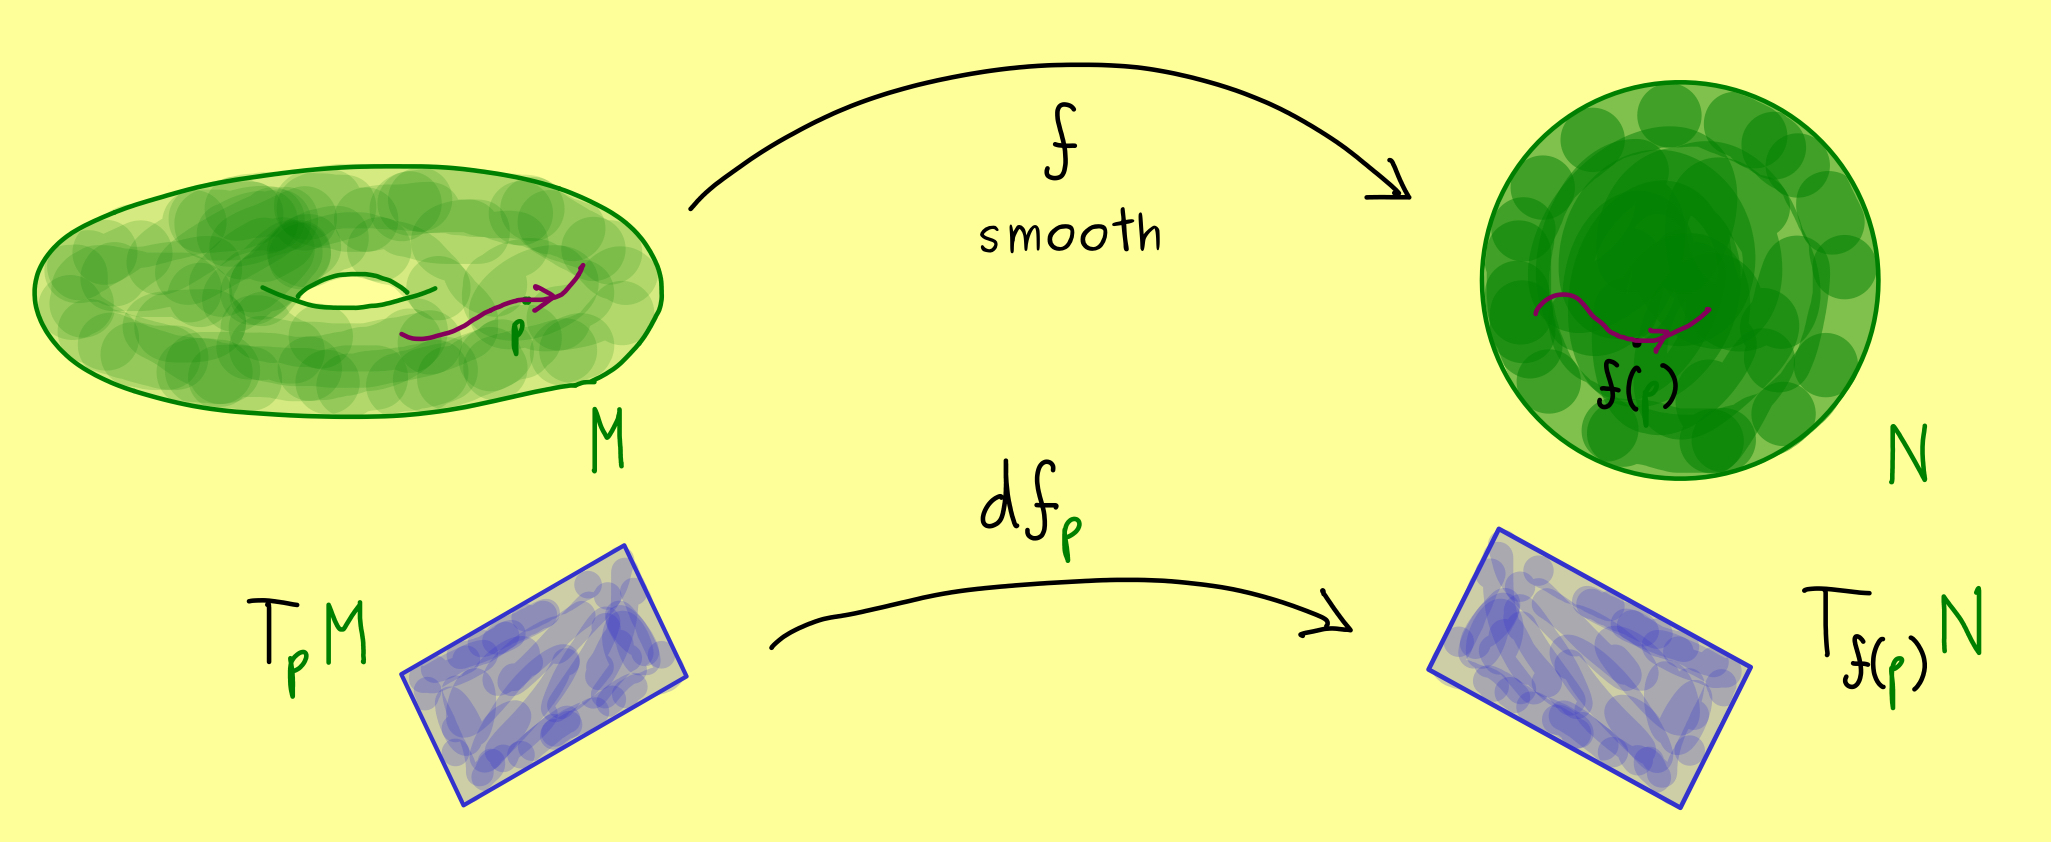
\includegraphics[width=0.7\textwidth]{Figs/differential_of_a_map_between_manifolds.jpeg}
    \caption{Differential of a smooth map}
\end{figure}

\begin{definition}{\textbf{Differential of f at point p}} \\
    Let \( f: M \to N \) be a smooth map between two smooth manifolds. \\
    Let \( p \in M \) and \( [\gamma] \in T_pM \). The differential of \( f \) at \( p \) is defined as \\
    \begin{equation*}
        df_p([\gamma]) = [f \circ \gamma] \in T_{f(p)}N
    \end{equation*}
\end{definition}

The linear map given by the differential is a linear approximation of the map \( f \) at the point \( p \). 

\begin{definition}{\textbf{Differential}} \\
    \begin{equation*}
        df : M \to TN \quad \text{defined as} \quad df(p) = df_p
    \end{equation*}
\end{definition}

\bigbreak

Example for submanifolds: \\
Let \( M , N \) be submanifolds of \( \mathbb{R}^n \), $p \in M$ and \( f: M \to N \) be a smooth map. \\
In this case, \(T_{f(p)}N = T_{f(p)}^{sub}N \). \\
$df_p ([\gamma]_{\sim}) = [f \circ \gamma_p]_{\sim} \stackrel{\text{bijection}}{=} (f \circ \gamma_p)'(0)$

\bigbreak

Example for $f : \mathbb{R}^n \to \mathbb{R}$ a smooth map: \\
$df_p([\gamma]_{\sim}) = (f \circ \gamma)'(0) = J_f(\gamma(0)) \cdot \gamma'(0) = \nabla f(p) \cdot \gamma'(0)$ \\
and we get that it's exactly the directional derivative of $f$ at $p$ along $[\gamma]$.

% * * * * * * * * * * * * * * * * * * * * * * * *
% * * * * * * * * * * * * * * * * * * * * * * * *
% * * * * * * * * * * * * * * * * * * * * * * * *
% * * * * * * * * * * * * * * * * * * * * * * * *
% * * * * * * * * * * * * * * * * * * * * * * * *
% * * * * * * * * * * * * * * * * * * * * * * * *
% * * * * * * * * * * * * * * * * * * * * * * * *

\section{Differential in Local charts}

Let \( f: M \to N \) be a smooth map from n-dimensional smooth manifold \( M \) to m-dimensional smooth manifold \( N \). \\
Let $p \in M$ and $(U, h)$ be a chart of $M$ at $p$ and $(V, k)$ be a chart of $N$ at $f(p)$. \\
\( \tilde{f} := k \circ f \circ h^{-1} : h(U) \to k(V) \) is a smooth map between open sets in \( \mathbb{R}^n \) and \( \mathbb{R}^m \). \\
\( k \circ f = \tilde{f} \circ h \). \\
Let $[\gamma] \in T_pM$ and $\gamma : (-\epsilon, \epsilon) \to M$ be a smooth curve with $\gamma(0) = p$. Then\\
 \begin{align*}
    dk_{f(p)}(df_p([\gamma])) &= dk_{f(p)}([f \circ \gamma]_{\sim}) \\
    &= [k \circ f \circ \gamma]_{\sim} \\&= (k \circ f \circ \gamma)'(0) \\
    &= (\tilde{f} \circ h \circ \gamma)'(0) \\&\stackrel{\tilde{f} : \mathbb{R}^n \to \mathbb{R}^m}{=} J_{\tilde{f}}(h(p)) \cdot (h \circ \gamma)'(0) \\
    &= J_{\tilde{f}}(h(p)) \cdot [\gamma \circ h]_\sim \\&= J_{\tilde{f}}(h(p)) \cdot dh_p([\gamma]_\sim)
 \end{align*}

Then after multipling by $k^{-1}$ we get that \\
\begin{empheq}[box=\fbox]{align*}
    f &= k^{-1} \circ \tilde{f} \circ h \\
    df &= dk^{-1} \circ J_{\tilde{f}} \circ dh 
\end{empheq}
   
The differential of the abstract smooth map $f$ is given as the Jacobian matrix in local charts.
The definitions with the the abstract tangent vectors were the correct way to generalize a differential.

\begin{figure}[H]
    \centering
    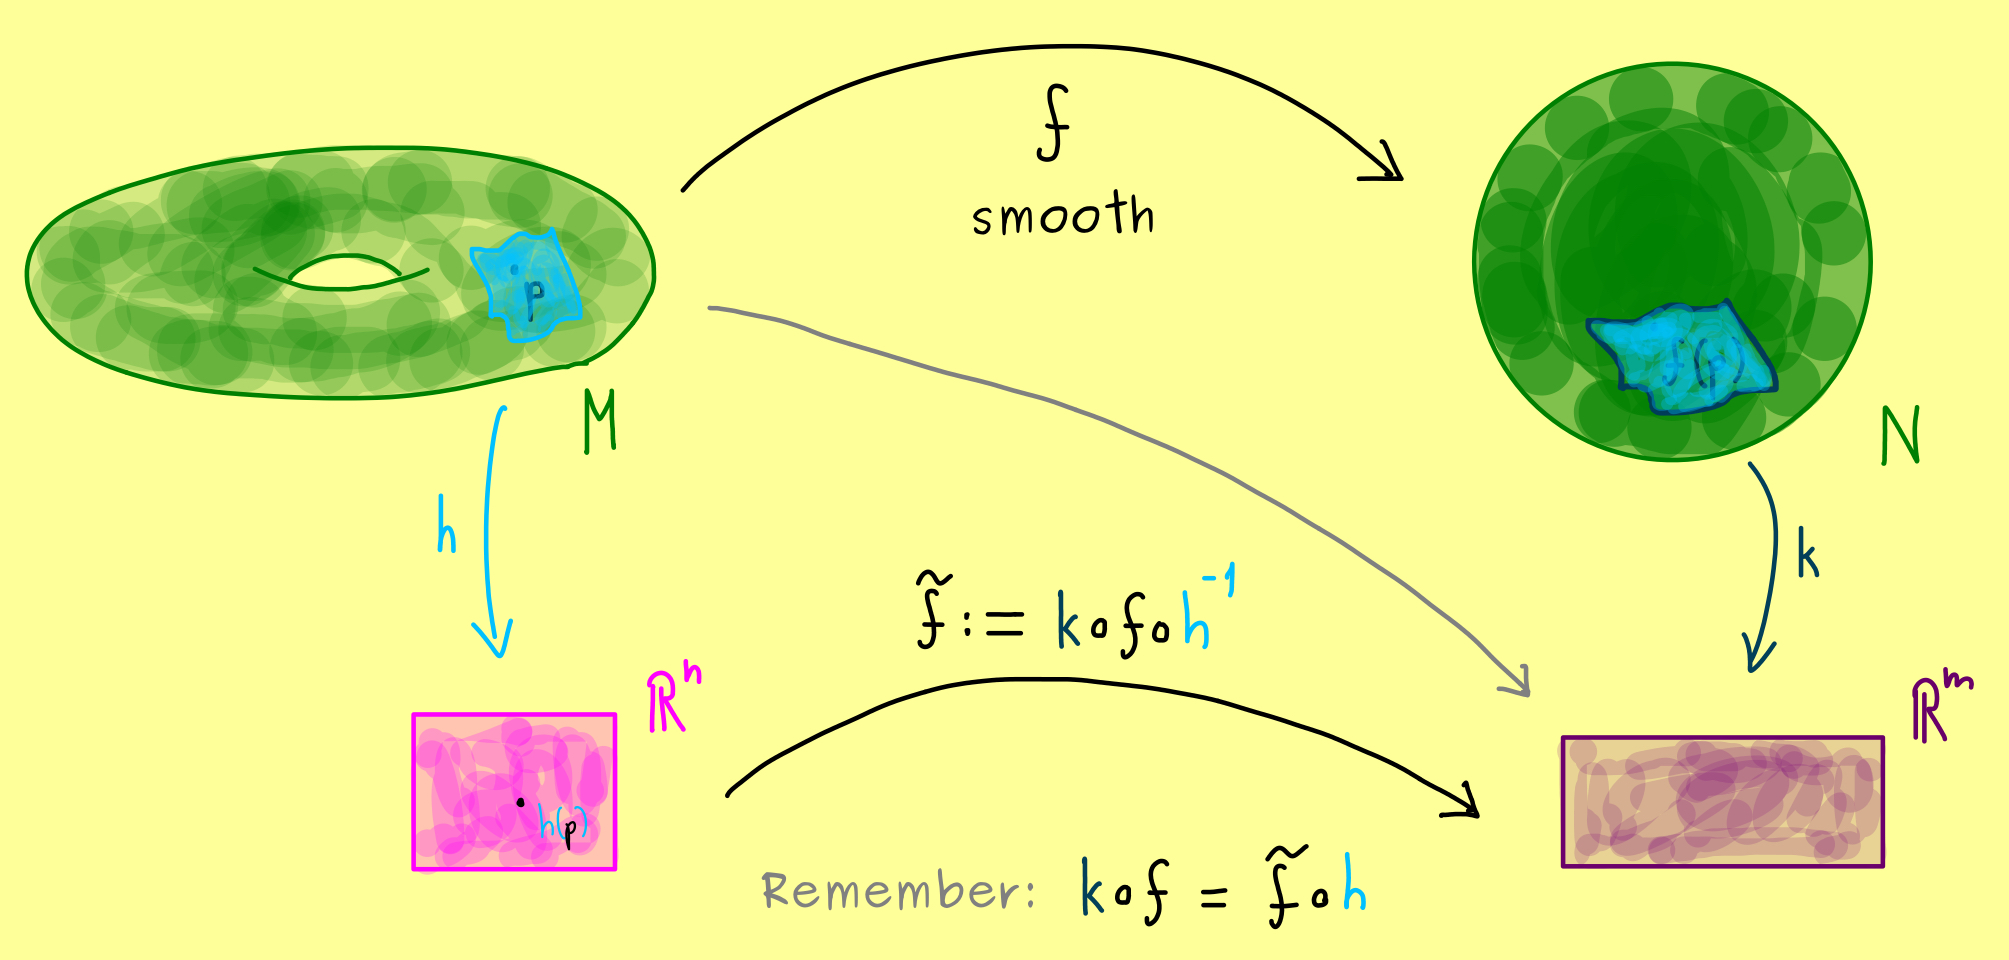
\includegraphics[width=0.8\textwidth]{Figs/differential_in_local_charts.jpeg}
    \caption{Differential in local charts}
\end{figure}


% * * * * * * * * * * * * * * * * * * * * * * * *
% * * * * * * * * * * * * * * * * * * * * * * * *
% * * * * * * * * * * * * * * * * * * * * * * * *
% * * * * * * * * * * * * * * * * * * * * * * * *
% * * * * * * * * * * * * * * * * * * * * * * * *
% * * * * * * * * * * * * * * * * * * * * * * * *
% * * * * * * * * * * * * * * * * * * * * * * * *

\section{Differential (example)}

We have previously defined the map $h_* : T_pM \to \mathbb{R}^n$ as $h_*([\gamma]_{\sim}) = (h \circ \gamma)'(0)$. \\
We have seen that $df_p([\gamma]_{\sim}) = [f \circ \gamma]_{\sim}$, and if the range of $f$ is a submanifold, then $df_p([\gamma]_{\sim}) = (f \circ \gamma)'(0)$. \\


Recall: for \( p \in M \) and $(U, h)$ the coordinate basis $\{ \partial_1, \ldots, \partial_n \}$ of $T_pM$ with respect to $(U, h)$
is given by $(\partial_1, \ldots, \partial_n)$ where $\partial_j := \varphi_*(e_j) = d\varphi_{h(p)}(e_j)$. \\ 

Directional derivative: \\
Let $f : M \to \mathbb{R}$ be a smooth map and $p \in M$. \\
In general, $df_p([\gamma]_{\sim})$ gives us a directional derivative. Then for partial derivatives $\partial_j f(p)$ we have $\tilde{\gamma}(t) = h(p) + t * e_j$ and \\
\begin{align*}
    \partial_j f(p) &:= df_p(\partial_j) \\
    &= df_p(d\varphi_{h(p)}(e_j)) \\
    &= [f \circ \varphi \circ \tilde{\gamma}]_{\sim} \\
    &= (f \circ \varphi \circ \tilde{\gamma})'(0) \\
    &= J_{f \circ \varphi}(h(p)) \cdot \tilde{\gamma}'(0) = \frac{\partial (f \circ \varphi)}{\partial x_j}(h(p))
\end{align*}



% * * * * * * * * * * * * * * * * * * * * * * * *
% * * * * * * * * * * * * * * * * * * * * * * * *
% * * * * * * * * * * * * * * * * * * * * * * * *
% * * * * * * * * * * * * * * * * * * * * * * * *
% * * * * * * * * * * * * * * * * * * * * * * * *
% * * * * * * * * * * * * * * * * * * * * * * * *
% * * * * * * * * * * * * * * * * * * * * * * * *

\section{Ricci calculus / Tensor calculus}

In Ricci calculus, we are calulating in the coordinates of a parametrization of a manifold. \\
Moreover, the poisition of indices in the notation is important (superscript indices are contravariant and subscript indices are covariant). \\

\begin{center} 
\begin{tabular}{|m{0.5\textwidth}|m{0.5\textwidth}|}
    \hline
    \multicolumn{1}{|c|}{\textbf{Our Language}} & \multicolumn{1}{c|}{\textbf{Ricci Calculus}} \\ 
    \hline
    components of a given chart $(U, h), h : U \to \mathbb{R}^n$ 
    & $h^j : U \to \mathbb{R}$ coordinates, or simply: $x^1, \ldots, x^n$ 
    \\ 
    \hline
    coordinate basis of $T_pM$: $\partial_j := \varphi_*(e_j)$
    & $\frac{\partial}{\partial x^1}, \ldots, \frac{\partial}{\partial x^n}$ 
    \\
    \hline
    tangent vector $[\gamma]_{\sim} \in T_pM$: $v_1 \partial_1 + \ldots + v_n \partial_n$
    & $v^1 \frac{\partial}{\partial x^1} + \ldots + v^n \frac{\partial}{\partial x^n} := v^j \frac{\partial}{\partial x^j}$ \\ &
    (Einsteins summation convention) ($\sum_{j=1}^{n} v^j \frac{\partial}{\partial x^j}$)
    \\
    \hline
    Inner product on $T_pM$: $\langle v, w\rangle \in \mathbb{R}$
    & $v^j g_{jk} w^k \in \mathbb{R}$ (metric tensor $g_{jk}$)
    \\
    \hline
\end{tabular}
\end{center}

We will deep dive later to the meaning of contravariant and covariant vectors, but for now:
\begin{itemize}
    \item Tangent vector is called contravariant vector in Ricci calculus.
\end{itemize}

\begin{definition}{\textbf{Contravariant vector}} \\
    A contravariant vector is a vector that transforms according to the rule: \\
    \begin{equation*}
        v^j \frac{\partial}{\partial x^j} \quad \text{where} \quad v^j \in \mathbb{R}
    \end{equation*}
\end{definition}

\begin{definition}{\textbf{Covariant vector}} \\
    A covariant vector is a vector that transforms according to the rule: \\
    \begin{equation*}
        v_j dx^j \quad \text{where} \quad v_j \in \mathbb{R}
    \end{equation*}
\end{definition}

Dual to a contravariant vector: $v_j dx^j$\\
For exmaple, the one-form for a vector in the tangent space: \\
In our language, $dx_j(\partial_k) = \delta_{jk}$, where $\delta_{jk}$ is the Kronecker delta.\\
In Ricci calculus, $dx^j(\frac{\partial}{\partial x^k}) = \delta^j_k$.



% * * * * * * * * * * * * * * * * * * * * * * * *
% * * * * * * * * * * * * * * * * * * * * * * * *
% * * * * * * * * * * * * * * * * * * * * * * * *
% * * * * * * * * * * * * * * * * * * * * * * * *
% * * * * * * * * * * * * * * * * * * * * * * * *
% * * * * * * * * * * * * * * * * * * * * * * * *
% * * * * * * * * * * * * * * * * * * * * * * * *

\section{Alternating k-forms}

\begin{definition}{\textbf{Dual Space (of a tangent space)}} \\
    Let \( M \) be an n-dimensional smooth manifold. \\
    The dual space of the tangent space of \( M \) at \( p \) is defined as
    \begin{equation*}
        T_p^*M := (T_pM)^* = \{ \alpha : T_pM \to \mathbb{R} \quad | \quad \alpha \quad \text{is linear} \}
    \end{equation*}
\end{definition}

For example, the one-form $dx_{j,p} : T_pM \to \mathbb{R}$ is defined as $dx_{j,p}(\partial_k) = \delta_{jk}$.

\begin{definition}{\textbf{Differential form}} \\
    A differential form on a smooth manifold \( M \) is a map $\omega$ defined on $M$ such that for each $p \in M$,
    $\omega(p)$ is a linear map $\omega_p : T_pM \to \mathbb{R}$.
\end{definition}

An example for a differential form is the one-form: $dx_j : p \mapsto dx_{j,p} \in T_p^*M$.

\begin{definition}{\textbf{k-linear (multilinear) map}} \\
    A map $f : V_1 \times \ldots \times V_k \to W$ is called k-linear if it is linear in each argument. \\ 
    That is, for each $i \in \{1, \ldots, k\}$, \\
    $f(v_1, \ldots, v_{i-1}, \lambda v_i + \mu v_i', v_{i+1}, \ldots, v_k) = \lambda f(v_1, \ldots, v_{i-1}, v_i, v_{i+1}, \ldots, v_k) + \mu f(v_1, \ldots, v_{i-1}, v_i', v_{i+1}, \ldots, v_k)$.
\end{definition}

\begin{definition}{\textbf{k-form}} \\
    Let \(V \) be a vector space. 
    A k-form on \( V \) is a k-linear map $\omega : V^k \to \mathbb{R}$.
\end{definition}

For exmaple, any inner product on a vector space \( V \) is a 2-form on \( V \) (bilinear form).

\begin{definition}{\textbf{Alternating k-form on $V$}} \\
    A k-form $\omega$ on \( V \) is called alternating if one of those conditions hold:
    \begin{itemize}
        \item $\omega(v_1, \ldots, v_k) = 0$ if $v_i = v_j$ for some $i \neq j$.
        \item $\omega(v_{\sigma(1)}, \ldots, v_{\sigma(k)}) = \text{sgn}(\sigma) \cdot \omega(v_1, \ldots, v_k)$ for each permutation $\sigma$ of $\{1, \ldots, k\}$. \\
            For example, $\omega(v_2, v_1, v_3) = -\omega(v_1, v_2, v_3)$.
        \item $\omega(v_1, \ldots, v_k) = 0$ if $v_i = \sum_{j=1}^{k} \lambda_j v_j$ for some $\lambda_j \in \mathbb{R}$ (linearly dependent vectors).
    \end{itemize}
\end{definition}

\begin{definition}{\textbf{$Alt^k(V)$}} \\
    Let \( V \) be a vector space. \\ 
    \begin{align*}
        Alt^k(V) &:= \{ \alpha : V^k \to \mathbb{R} \quad | \quad \omega \quad \text{is k-linear and alternating} \}
    \end{align*}
\end{definition}

Examples: 
\begin{itemize}
    \item $det \in Alt^n(\mathbb{R}^n)$ is an alternating n-form on $\mathbb{R}^n$.
    \item $Alt^1(V) = { \alpha : V \to \mathbb{R} \quad | \quad \alpha \quad \text{is linear} } = V^*$ is the dual space of \( V \).
    \item $Alt^0(V) = \mathbb{R}$.
\end{itemize}


% * * * * * * * * * * * * * * * * * * * * * * * *
% * * * * * * * * * * * * * * * * * * * * * * * *
% * * * * * * * * * * * * * * * * * * * * * * * *
% * * * * * * * * * * * * * * * * * * * * * * * *
% * * * * * * * * * * * * * * * * * * * * * * * *
% * * * * * * * * * * * * * * * * * * * * * * * *
% * * * * * * * * * * * * * * * * * * * * * * * *

\section{Wedge Product}

\begin{definition}{\textbf{Wedge product}} \\
    Let \( V \) be a vector space and \( \alpha \in Alt^k(V) \) and \( \beta \in Alt^s(V) \). \\
    The wedge product \( \wedge : Alt^k(V) \times Alt^s(V) \to Alt^{k+s}(V) \) is defined as
    \begin{align*}
        \wedge(\alpha, \beta) &\to \alpha \wedge \beta : V^{k+l} \to \mathbb{R} \quad \text{defined as} \\
        \alpha \wedge \beta(v_1, \ldots, v_{k+s}) &= \frac{1}{k! \cdot s!} \sum_{\sigma \in S_{k+s}} \text{sgn}(\sigma) \cdot \alpha(v_{\sigma(1)}, \ldots, v_{\sigma(k)}) \cdot \beta(v_{\sigma(k+1)}, \ldots, v_{\sigma(k+s)})
    \end{align*}
\end{definition}

Examples: 
\begin{itemize}
    \item $\alpha, \beta \in Alt^1(V) = V^*$. Then $\alpha \wedge \beta \in Alt^2(V)$, is a 2-form on \( V \) that is defined 
    as $\alpha \wedge \beta(v_1, v_2) = \alpha(v_1) \cdot \beta(v_2) - \alpha(v_2) \cdot \beta(v_1)$.
    
    
    \item $\alpha , \beta \in Alt^1(\mathbb{R}^3), \quad 
    \alpha ( \begin{pmatrix}
        x1 \\ x2 \\ x3
    \end{pmatrix}) = x1, \quad
    \beta ( \begin{pmatrix}
        x1 \\ x2 \\ x3
    \end{pmatrix}) = x2$. \\
    Then $\alpha \wedge \beta \in Alt^2(\mathbb{R}^3)$ is defined as
    \begin{align*}
        \alpha \wedge \beta ( \begin{pmatrix}
            x1 \\ x2 \\ x3
        \end{pmatrix}, \begin{pmatrix}
            y1 \\ y2 \\ y3
        \end{pmatrix}) &=  x1 \cdot y2 - y1 \cdot x2 = 
        \langle 
        \begin{pmatrix}
            x1 \\ x2 \\ x3
        \end{pmatrix}
        ,
        \begin{pmatrix}
            0 & 1 & 0 \\
            -1 & 0 & 0 \\
            0 & 0 & 0 \\
        \end{pmatrix}
        \begin{pmatrix}
            y1 \\ y2 \\ y3
        \end{pmatrix}
        \rangle
    \end{align*}

    and the matrix $\begin{pmatrix}
        0 & 1 & 0 \\
        -1 & 0 & 0 \\
        0 & 0 & 0 \\
    \end{pmatrix}$ is the matrix identified with the 2-form $\alpha \wedge \beta$.
\end{itemize}

\paragraph{Properties of the wedge product:}
\begin{enumerate}
    \item Anticommutative: $\alpha \wedge \beta = (-1)^{k \cdot s} \cdot \beta \wedge \alpha$.
    \item Bilinear:
        \begin{itemize}
            \item $(\alpha + \beta) \wedge \gamma = \alpha \wedge \gamma + \beta \wedge \gamma$.
            \item $\lambda (\cdot \alpha) \wedge \beta = \lambda \cdot (\alpha \wedge \beta)$.
        \end{itemize}
    \item Associative: $(\alpha \wedge \beta) \wedge \gamma = \alpha \wedge (\beta \wedge \gamma)$.
    \item Pullback: for a linear map $f : W \to V$, and $\alpha \in Alt^k(V)$, $(f^* \alpha)(w_1, \ldots, w_k) = \alpha(f(w_1), \ldots, f(w_k))$. \\
        $f^*(\alpha \wedge \beta) = f^* \alpha \wedge f^* \beta$.
\end{enumerate}


The wedge product of two vectors, \(\mathbf{u}\) and \(\mathbf{v}\), represented as \(\mathbf{u} \wedge \mathbf{v}\), 
can be interpreted geometrically as the oriented area of the parallelogram spanned by these two vectors. 
The orientation is significant because swapping the vectors reverses the sign of the resulting area.

Mathematically, if \(\mathbf{u} = ai + bj\) and \(\mathbf{v} = ci + dj\), where i and j are basis vectors, then the wedge product is defined as:

\begin{align*}
    i \wedge i = 0, \quad j \wedge j = 0
\end{align*}

\begin{align*}
    0 = (i + j) \wedge (i + j) = i \wedge i + i \wedge j + j \wedge i + j \wedge j = i \wedge j + j \wedge i \Rightarrow i \wedge j = -j \wedge i
\end{align*}

\begin{align*}
\mathbf{u} \wedge \mathbf{v} &= (ai + bj) \wedge (ci + dj) \\
&= ai \wedge ci + ai \wedge dj + bj \wedge ci + bj \wedge dj \\
&= ac i \wedge i + ad i \wedge j + bc j \wedge i + bd j \wedge j \\
&= (ad - bc) i \wedge j
\end{align*}



% * * * * * * * * * * * * * * * * * * * * * * * *
% * * * * * * * * * * * * * * * * * * * * * * * *
% * * * * * * * * * * * * * * * * * * * * * * * *
% * * * * * * * * * * * * * * * * * * * * * * * *
% * * * * * * * * * * * * * * * * * * * * * * * *
% * * * * * * * * * * * * * * * * * * * * * * * *
% * * * * * * * * * * * * * * * * * * * * * * * *

\section{Differential forms}

\begin{definition}{\textbf{k-form on the manifold}} \\
    A k-form on a smooth manifold \( M \) is a map 
    \begin{align*}
        \omega &: M \to \cup_{p \in M} Alt^k(T_pM) \\
        p &\mapsto \omega_p = w(p) \in Alt^k(T_pM)
    \end{align*}
\end{definition}

\bigbreak

We also define: $\omega \wedge \eta : M \to \cup_{p \in M} Alt^{k+s}(T_pM)$ as $(\omega \wedge \eta)_p := \omega_p \wedge \eta_p$. 
\medbreak
For any smooth map $f : M \to N$, we define $f^* \omega : M \to \cup_{p \in M} Alt^k(T_pM)$ as \\
$(f^* \omega)(p) := (df_p)^* \omega_{p}$.

\paragraph{Basis elements}: \\
Recall, For a chart $(U, h)$ of $M$ at $p$, the coordinate basis of $T_pM$ is $( \partial_1, \ldots, \partial_n )$, with $\partial_j = \varphi_*(e_j) = d\varphi_{h(p)}(e_j)$. \\
Then, the dual basis of $(T_pM)* = Alt^1(T_pM)$ is $( dx_p^1, \ldots, dx_p^n )$ where $dx_p^j(\partial_k) = \delta_k^j$.

\begin{definition}\textbf{Basis elements of k-forms} \\
    Let $dx_p^1, \ldots, dx_p^n$ be the dual basis of $T_pM$ at $p$. \\
    The basis elements of $Alt^k(T_pM)$ are defined as
    \begin{align*}
        &(dx_p^{\mu_1} \wedge \ldots \wedge dx_p^{\mu_k})_{\mu_1 < \mu_2 < \ldots < \mu_k} : T_pM^k \to \mathbb{R} 
    \end{align*}
\end{definition}

Example: $dim(M) = 3$, then the basis elements of $Alt^2(T_pM)$ are $(dx_p^1 \wedge dx_p^2, dx_p^1 \wedge dx_p^3, dx_p^2 \wedge dx_p^3)$.

\bigbreak

Conclusion: \\
Each k-form on a manifold M can locally be written as a linear combination of the basis elements of $Alt^k(T_pM)$:
\begin{equation*}
    \omega(p) = \sum_{\mu_1 < \ldots < \mu_k} \omega_{\mu_1, \ldots, \mu_k}(p) \cdot dx_p^{\mu_1} \wedge \ldots \wedge dx_p^{\mu_k}
\end{equation*}
Each $\omega_{\mu_1, \ldots, \mu_k} : U \to \mathbb{R}$ is called a component function of $\omega$ in the chart $(U, h)$.

\begin{definition}{\textbf{Differentible k-form on M}} \\
    A k-form $\omega$ on a smooth manifold \( M \) is called differentiable if for each chart $(U, h)$ of \( M \), 
    the component functions $\omega_{\mu_1, \ldots, \mu_k}$ are differentiable. \\
    We denote the set of all differentiable k-forms on \( M \) as \( \Omega^k(M) \).
    We define \( \Omega^0(M) = C^{\infty}(M) \).
\end{definition}



% * * * * * * * * * * * * * * * * * * * * * * * *
% * * * * * * * * * * * * * * * * * * * * * * * *
% * * * * * * * * * * * * * * * * * * * * * * * *
% * * * * * * * * * * * * * * * * * * * * * * * *
% * * * * * * * * * * * * * * * * * * * * * * * *
% * * * * * * * * * * * * * * * * * * * * * * * *
% * * * * * * * * * * * * * * * * * * * * * * * *

\section{Examples of differential forms}

M = $\mathbb{R}^2$ , $\partial_1 = \frac{\partial}{\partial x} = \begin{pmatrix} 1 \\ 0 \end{pmatrix}$, $\partial_2 = \frac{\partial}{\partial y} = \begin{pmatrix} 0 \\ 1 \end{pmatrix}$, 
$dx_p^1 = \begin{pmatrix} 1 & 0 \end{pmatrix}$, $dx_p^2 = \begin{pmatrix} 0 & 1 \end{pmatrix}$ \\
\begin{align*}
    dx_p^1 \wedge dx_p^2 ( \begin{pmatrix} a_{1,1} \\ a_{2,1} \end{pmatrix}, \begin{pmatrix} a_{1,2} \\ a_{2,2} \end{pmatrix}) &=  
    \sum_{\sigma \in S_2} \text{sgn}(\sigma) \cdot dx_p^1(\begin{pmatrix} a_{1, \sigma(1)} \\ a_{2, \sigma(1)} \end{pmatrix}) \cdot dx_p^2(\begin{pmatrix} a_{1, \sigma(2)} \\ a_{2, \sigma(2)} \end{pmatrix}) 
    \\&= \sum_{\sigma \in S_2} \text{sgn}(\sigma) \cdot a_{1, \sigma(1)} \cdot a_{2, \sigma(2)} 
    \\&= det \begin{pmatrix} a_{1,1} & a_{1,2} \\ a_{2,1} & a_{2,2} \end{pmatrix}
\end{align*}

In general for $\mathbb{R}^n$, $dx_p^{\mu_1} \wedge \ldots \wedge dx_p^{\mu_k} ( \begin{pmatrix} a_{1,1} \\ \vdots \\ a_{n,1} \end{pmatrix}, \ldots, \begin{pmatrix} a_{1,k} \\ \vdots \\ a_{n,k} \end{pmatrix}) = det \begin{pmatrix} a_{1,1} & \ldots & a_{1,k} \\ \vdots & \ddots & \vdots \\ a_{n,1} & \ldots & a_{n,k} \end{pmatrix}$

\bigbreak

M = $\mathbb{R}^2$, $\varphi : (r, \theta) \to \mathbb{R}^2$, $\varphi(r, \theta) = \begin{pmatrix} r \cdot cos(\theta) \\ r \cdot sin(\theta) \end{pmatrix}$ \\
$\partial_1(r, \theta) = \frac{\partial \varphi }{\partial r}(r, \theta) = \begin{pmatrix} cos(\theta) \\  sin(\theta) \end{pmatrix}$, 
$\partial_2(r, \theta) = \frac{\partial  \varphi}{\partial \theta}(r, \theta) = \begin{pmatrix} -r \cdot sin(\theta) \\ r \cdot cos(\theta) \end{pmatrix}$ \\
The corresponding dual basis is $dr_p = \begin{pmatrix} cos(\theta) & sin(\theta) \end{pmatrix}$, $d\theta_p = \frac{1}{r} \begin{pmatrix} - \cdot sin(\theta) & \cdot cos(\theta) \end{pmatrix}$ \\
for $p = (x, y)$, $dr_p = \begin{pmatrix} \frac{x}{\sqrt{x^2 + y^2}} & \frac{y}{\sqrt{x^2 + y^2}} \end{pmatrix}$, $d\theta_p = \begin{pmatrix} - \frac{y}{x^2 + y^2} & \frac{x}{x^2 + y^2} \end{pmatrix}$ \\
Then $(dr_p \wedge d\theta_p) (e_1, e_2) = dr_p(e_1) \cdot d\theta_p(e_2) - dr_p(e_2) \cdot d\theta_p(e_1) = \frac{1}{r} (\cos^2(\theta) + \sin^2(\theta)) = \frac{1}{r}$

% * * * * * * * * * * * * * * * * * * * * * * * *
% * * * * * * * * * * * * * * * * * * * * * * * *
% * * * * * * * * * * * * * * * * * * * * * * * *
% * * * * * * * * * * * * * * * * * * * * * * * *
% * * * * * * * * * * * * * * * * * * * * * * * *
% * * * * * * * * * * * * * * * * * * * * * * * *
% * * * * * * * * * * * * * * * * * * * * * * * *

\section{Orientable manifolds}

For example. $\mathbb{R}^n$ with basis $(e_1, \ldots, e_n)$ is oriented by the basis $(e_1, \ldots, e_n)$. \\
For change of basis matrix $T_{C \leftarrow B}$, 
$det(T_{C \leftarrow B}) > 0$ means that the basis $C$ is positively oriented with respect to the basis $B$, 
and $det(T_{C \leftarrow B}) < 0$ means that the basis $C$ is negatively oriented with respect to the basis $B$. \\
\medbreak
Thus, there are two equivalence classes of bases: positively and negatively oriented bases with respect to the standard basis. \\

\begin{definition}{\textbf{Orientation in vector spaces}} \\
    An orientation $(V, or)$ is a tuple of V finite-dimensional vector space and a choice of an equivalence class of bases. \\
\end{definition}

Let M be an n-dimensional smooth manifold, and $p \in M$. \\
Let \(U, h\) be a chart of \(M\) at \(p\), and $\varphi_* : \mathbb{R}^n \to T_pM$ be the differential of the chart map, $e_j \to \partial_j^{h}(p)$. \\

\begin{definition}{\textbf{Orientable manifold}} \\
    A smooth manifold \( M \) is called orientable if there is a family of orientations for the tangent spaces $\{(T_pM, or_p)\}_{p \in M}$ such that
    $\forall p \in M, \exists (U,h) \quad \text{chart of} \quad M \quad \text{at} \quad p$ such that $\forall x \in U$: $(\partial_1^h(x), \ldots, \partial_n^h(x)) \in or x$.
\end{definition}

% * * * * * * * * * * * * * * * * * * * * * * * *
% * * * * * * * * * * * * * * * * * * * * * * * *
% * * * * * * * * * * * * * * * * * * * * * * * *
% * * * * * * * * * * * * * * * * * * * * * * * *
% * * * * * * * * * * * * * * * * * * * * * * * *
% * * * * * * * * * * * * * * * * * * * * * * * *
% * * * * * * * * * * * * * * * * * * * * * * * *

\todo[inline]{complete the orientation section}
% \section{Alternative definitions for orientation}


% * * * * * * * * * * * * * * * * * * * * * * * *
% * * * * * * * * * * * * * * * * * * * * * * * *
% * * * * * * * * * * * * * * * * * * * * * * * *
% * * * * * * * * * * * * * * * * * * * * * * * *
% * * * * * * * * * * * * * * * * * * * * * * * *
% * * * * * * * * * * * * * * * * * * * * * * * *
% * * * * * * * * * * * * * * * * * * * * * * * *

\section{Riemannian metrics}

% * * * * * * * * * * * * * * * * * * * * * * * *
% * * * * * * * * * * * * * * * * * * * * * * * *
% * * * * * * * * * * * * * * * * * * * * * * * *
% * * * * * * * * * * * * * * * * * * * * * * * *
% * * * * * * * * * * * * * * * * * * * * * * * *
% * * * * * * * * * * * * * * * * * * * * * * * *
% * * * * * * * * * * * * * * * * * * * * * * * *

% \section{Examples for Riemannian Manifolds}

% * * * * * * * * * * * * * * * * * * * * * * * *
% * * * * * * * * * * * * * * * * * * * * * * * *
% * * * * * * * * * * * * * * * * * * * * * * * *
% * * * * * * * * * * * * * * * * * * * * * * * *
% * * * * * * * * * * * * * * * * * * * * * * * *
% * * * * * * * * * * * * * * * * * * * * * * * *
% * * * * * * * * * * * * * * * * * * * * * * * *

% \section{Canonical Volume Form}




% * * * * * * * * * * * * * * * * * * * * * * * * 
% * * * * * * * * * * * * * * * * * * * * * * * * 
% * * * * * * * * * * * * * * * * * * * * * * * * 
% * * * * * * * * * * * * * * * * * * * * * * * * 
% * * * * * * * * * * * * * * * * * * * * * * * * 
% * * * * * * * * * * * * * * * * * * * * * * * * 
% * * * * * * * * * * * * * * * * * * * * * * * * 
% * * * * * * * * * * * * * * * * * * * * * * * * 
% * * * * * * * * * * * * * * * * * * * * * * * * 
% * * * * * * * * * * * * * * * * * * * * * * * * 
% * * * * * * * * * * * * * * * * * * * * * * * * 
% * * * * * * * * * * * * * * * * * * * * * * * * 
% * * * * * * * * * * * * * * * * * * * * * * * * 
% * * * * * * * * * * * * * * * * * * * * * * * * 
% * * * * * * * * * * * * * * * * * * * * * * * * 
% * * * * * * * * * * * * * * * * * * * * * * * * 
% * * * * * * * * * * * * * * * * * * * * * * * * 
% * * * * * * * * * * * * * * * * * * * * * * * * 
% * * * * * * * * * * * * * * * * * * * * * * * * 


\chapter{The First Miracle: Robustness}

Let f be a convex function, and let $x^*$ be a minimizer of f. 

\section{Gradient Descent}
\begin{definition}{Gradient Descent} \\
    \begin{equation}
       x_{t+1} = x_t - \eta \nabla f(x_t) 
    \end{equation}
\end{definition}

It holds that:
\begin{equation}
    f(x^*) \geq f(x_t) + \nabla f(x_t) \cdot (x^* - x_t)
\end{equation}

\begin{equation}
    0 \leq f(x_t) - f(x^*) \leq \nabla f(x_t) \cdot (x_t - x^*) 
\end{equation}

\subsection{Analysis of the Gradient Descent Algorithm}

\begin{align*}
    \|a\|^2  &= \|b\|^2 + \|a - b\|^2   \\ 
    \|b\|^2 &= \|a\|^2 - \|a - b\|^2 = \|a\|^2 - ( \|a\|^2 - 2a \cdot b + \|b\|^2  ) = 2 a \cdot b - \|b\|^2
\end{align*}
Then we have:
\begin{align*}
    \| x^* - x_t \|^2 - \| x^* - x_{t+1} \|^2 &= - 2 \eta (x^* - x_t) \cdot \nabla f(x_t) - \eta^2 \| \nabla f(x_t) \|^2 \\
    &= 2 \eta (x_t - x^*) \cdot \nabla f(x_t) - \eta^2 \| \nabla f(x_t) \|^2 \\
    &\geq  2 ( f(x_t) - f(x^*) ) - \eta^2 L^2
\end{align*}

Where the last inequality follows from the convexity and the Lipschitz continuity of $f$. 

\begin{figure}[H]
    \centering
    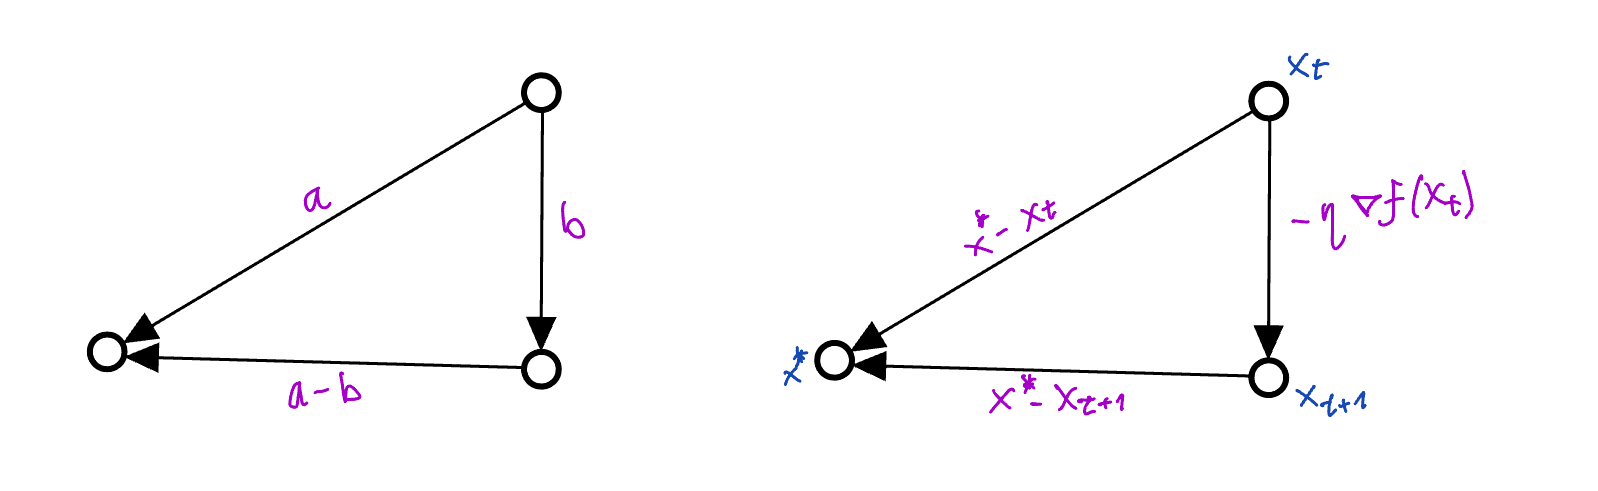
\includegraphics[width=0.8\textwidth]{Figs/vectors_triangle.jpeg}
    \caption{Gradient Descent}
\end{figure}

Then if we sum the above inequality from $t=1$ to $T$, we get:
\begin{align*}
    \sum_{t=1}^T ( f(x_t) - f(x^*) ) &\leq \frac{\|x_1 - x^*\|^2}{2 \eta} + \frac{\eta L^2}{2} T 
\end{align*}

In fact, this is a specific case of the Fundamental Inequality of Optimization. 

\begin{theorem}{Fundamental Inequality of Optimization (unconstrained version)} \\
    Suppose \( x_{t+1} = x_t - \eta g_t \) for all \( t \), where \( g_1, \ldots, g_T \in \mathbb{R}^d \) are arbitrary vectors. Then for all \( x^* \in \mathbb{R}^d \) it holds that
    \[
    \sum_{t=1}^T g_t \cdot (x_t - x^*) \leq \frac{\|x_1 - x^*\|^2}{2\eta} + \frac{\eta}{2} \sum_{t=1}^T \|g_t\|^2.
    \]
\end{theorem}
    
\begin{proof}{Fundamental Inequality of Optimization} \\
    The proof tracks \( \|x_t - x^*\|^2 \) as a ``potential''. First write
    \[
    \|x_{t+1} - x^*\|^2 = \|(x_t - x^*) - \eta g_t\|^2 = \|x_t - x^*\|^2 - 2\eta g_t \cdot (x_t - x^*) + \eta^2 \|g_t\|^2,
    \]
    that is,
    \[
    \|x_t - x^*\|^2 - \|x_{t+1} - x^*\|^2 = 2\eta g_t \cdot (x_t - x^*) - \eta^2 \|g_t\|^2.
    \]
    Summing over \( t = 1, \ldots, T \) and telescoping terms, we obtain
    \[
    \|x_1 - x^*\|^2 - \|x_{T+1} - x^*\|^2 = 2\eta \sum_{t=1}^T g_t \cdot (x_t - x^*) - \eta^2 \sum_{t=1}^T \|g_t\|^2.
    \]
    Organizing terms, we conclude:
    \[
    \sum_{t=1}^T g_t \cdot (x_t - x^*) \leq \frac{\|x_1 - x^*\|^2 - \|x_{T+1} - x^*\|^2}{2\eta} + \frac{\eta}{2} \sum_{t=1}^T \|g_t\|^2. \quad 
    \]
\end{proof}

\bigbreak


\todo[inline]{SGD , choosing eta} 
    

% * * * * * * * * * * * * * * * * * * * * * * * * 
% * * * * * * * * * * * * * * * * * * * * * * * * 
% * * * * * * * * * * * * * * * * * * * * * * * * 
% * * * * * * * * * * * * * * * * * * * * * * * * 
% * * * * * * * * * * * * * * * * * * * * * * * * 
% * * * * * * * * * * * * * * * * * * * * * * * * 
% * * * * * * * * * * * * * * * * * * * * * * * * 
% * * * * * * * * * * * * * * * * * * * * * * * * 
% * * * * * * * * * * * * * * * * * * * * * * * * 
% * * * * * * * * * * * * * * * * * * * * * * * * 
% * * * * * * * * * * * * * * * * * * * * * * * * 
% * * * * * * * * * * * * * * * * * * * * * * * * 
% * * * * * * * * * * * * * * * * * * * * * * * * 
% * * * * * * * * * * * * * * * * * * * * * * * * 
% * * * * * * * * * * * * * * * * * * * * * * * * 
% * * * * * * * * * * * * * * * * * * * * * * * * 
% * * * * * * * * * * * * * * * * * * * * * * * * 
% * * * * * * * * * * * * * * * * * * * * * * * * 
% * * * * * * * * * * * * * * * * * * * * * * * * 

\chapter{The Second Miracle: Potential Based}

\section{Experts Problem}

At each time step, the player picks an action $I_t \in [n]$ (we have n experts) and the adversary picks a loss vector $l_t \in {0,1}^n$. 
The player incurs loss $l_t(I_t)$ and the goal is to minimize the regret:
\begin{equation}
    \text{Regret}_T(i) = \sum_{t=1}^T \left( l_t(I_t) - l_t(i) \right)
\end{equation}

We consider the case where in each time step the player chooses an action from a distribution $\vec{p}$ over the $n$ experts (a vector from the simplex):
\begin{equation*}
    \vec{p} \in \mathcal{K} := \bigtriangleup_n = \{ \vec{p} \in \mathbb{R}_+^n : p_i \geq 0, \sum_{i=1}^n p_i = 1 \}
\end{equation*}

\subsubsection{Approach 1: Gradient Descent}
We can use gradient descent on $f_t(\vec{p}_t) = \vec{l_t} \cdot \vec{p}$, where $\vec{l_t}$ is the loss vector at time $t$.
It holds that $\nabla f_t(\vec{p}_t) = \vec{l_t}$. We can use the analysis of the gradient descent algorithm for gradient descent of convex functions varying in time.

Let $q \in \bigtriangleup_n$ be any distribution. Then we have:
\begin{align*}
    f_t(q) &\geq f_t(\vec{p}_t) + \nabla f_t(q) \cdot (q - \vec{p}_t) \Longrightarrow \\
    f_t(\vec{p}_t) - f_t(q) &\leq \nabla f_t(q) \cdot (\vec{p}_t - q) 
\end{align*}
Then:
\begin{align*}
    \| q - p_t \|^2 - \| q - p_{t+1} \|^2 &= - 2 \eta (q - p_t) \cdot \nabla f_t(p_t) - \eta^2 \| \nabla f_t(p_t) \|^2  \Longrightarrow \\
    f_t(\vec{p}_t) - f_t(q) &\leq \nabla f_t(q) \cdot (\vec{p}_t - q)  = \frac{1}{2\eta} \left( \| q - \vec{p}_t \|^2  - \| q - \vec{p}_{t+1} \|^2 \right) + \frac{\eta}{2} \| \nabla f_t(\vec{p}_t) \|^2 \Longrightarrow \\ 
    \sum_{t=1}^T \left( f_t(\vec{p}_t) - f_t(q) \right) &\leq \frac{1}{2\eta} \left( \| q - \vec{p}_1 \|^2 - \| q - \vec{p}_{T+1} \|^2 \right)+ \frac{\eta}{2} \sum_{t=1}^T \| \nabla f_t(\vec{p}_t) \|^2 \\
    &\leq \frac{1}{2\eta} \| q - \vec{p}_1 \|^2 + \frac{\eta}{2} \sum_{t=1}^T \| \nabla f_t(\vec{p}_t) \|^2 \\
    &\leq \frac{1}{\eta} + \frac{\eta}{2} T n  = \textbf{O} ( \sqrt{Tn} )
\end{align*}

We have used the facts that: 
\begin{itemize}
    \item Both $q$ and $\vec{p}_1$ are distributions, so $\| q - \vec{p}_1 \|^2 \leq 2$.
    \item $\| \nabla f_t(\vec{p}_t) \|^2 \leq n$ (as the loss vector is in ${0,1}^n$).
\end{itemize}

we can see that in this case, the rate of convergence DO depend on the dimension of the problem, in contrast to the non-varying case.
The fact that the rate of convergence DO NOT depend on the dimension of the problem in GD is one of the reasons why GD is so useful in practice.


\subsubsection{Approach 2: Multiplicative Weights Update (MWU)}

The optimal convergence rate for the experts problem is $\sqrt{T \log n}$, which is achieved by the MWU algorithm.
It is achieved by considering the sparsity of the OPT strategy (which is just a point mass on the best expert). 
We will modify GD such that it will move faster when far from a sparse point.

\medbreak

\todo[inline] {Approach 2: M}


\section{Mirror Descent}

Endow $\mathcal{K}$ with a Riemannian structure: \\
$<\cdot, \cdot>_x$ for each $x \in \mathcal{K}$, the tangent space will be $\mathbb{R}^n$. \\
\begin{align*}
    \text{Before:}\\
    x_{t+1} = x_t - \eta \nabla f(x_t) \rightarrow f(x + dx) &\approx f(x) + \langle \nabla f(x) , dx \rangle \\
    \text{Now:}\\
   f(x + dx) &\approx f(x) + \langle grad_M f(x) , dx \rangle_x
\end{align*}

We will consider $M$ such that $\langle \cdot, \cdot \rangle_x = \nabla^2 \phi [\cdot, \cdot]$, where $\phi$ is a fixed convex function. 
The function $\phi$ encodes the geometry of the space, and this is where the prior information is encoded. We get that:
\begin{align*}
    (dx)^T  \nabla f(x) = \langle grad_M f(x) , dx \rangle_x &= dx^T \nabla^2 \phi(x) grad_M f(x) \Rightarrow \\
    grad_M f(x) &= [\nabla^2 \phi(x)]^{-1} \nabla f(x)
\end{align*}

Idea: $x_{t+1} = x_t - \eta [\nabla^2 \phi(x_t)]^{-1} \nabla g_t $ \\
Question: what is the potential? (how do we analyze this algorithm?) \\
Miracle: the potential is the Bregman divergence of $\phi$ ($D_{\phi}(x, y) = \phi(x) - \phi(y) - \langle \nabla \phi(y), x-y \rangle_x$) [Nemiroski, 1979] 

\bigbreak

\begin{algorithm}[H]
    \SetNoFillComment
    \SetAlgoLined
    % \KwIn{} 
    % \KwOut{}
    $g : \mathbb{R}_+ \to \mathbb{R}^n$ is a smooth vector field \\
    \begin{align*}
        \frac{d}{dt} x_t &= -[\nabla^2 \phi(x_t)]^{-1} (\eta g(t) + \lambda (t))
    \end{align*}
    Where $\lambda(t) \in N_{\mathcal{K}}(x_t), x(t) \in \mathcal{K}$ is a lagrange multiplier - it is an element of the normal cone of $\mathcal{K}$ at $x_t$. \\
    \caption{Continues time Mirror Descent} \label{Continues time Mirror Descent}

    This is the same as the following: 
    \begin{align*}
        x(t + dt) = \argmin_{x \in \mathcal{K}} \left\{ \eta g(t) \cdot x + \frac{1}{2} \| x - x(t) \|^2_{\nabla^2 \phi(x_t)} \right\}
    \end{align*}
\end{algorithm}




% * * * * * * * * * * * * * * * * * * * * * * * * 
% * * * * * * * * * * * * * * * * * * * * * * * * 
% * * * * * * * * * * * * * * * * * * * * * * * * 
% * * * * * * * * * * * * * * * * * * * * * * * * 
% * * * * * * * * * * * * * * * * * * * * * * * * 
% * * * * * * * * * * * * * * * * * * * * * * * * 
% * * * * * * * * * * * * * * * * * * * * * * * * 
% * * * * * * * * * * * * * * * * * * * * * * * * 
% * * * * * * * * * * * * * * * * * * * * * * * * 
% * * * * * * * * * * * * * * * * * * * * * * * * 
% * * * * * * * * * * * * * * * * * * * * * * * * 
% * * * * * * * * * * * * * * * * * * * * * * * * 
% * * * * * * * * * * * * * * * * * * * * * * * * 
% * * * * * * * * * * * * * * * * * * * * * * * * 
% * * * * * * * * * * * * * * * * * * * * * * * * 
% * * * * * * * * * * * * * * * * * * * * * * * * 
% * * * * * * * * * * * * * * * * * * * * * * * * 
% * * * * * * * * * * * * * * * * * * * * * * * * 
% * * * * * * * * * * * * * * * * * * * * * * * * 

\chapter{The Third Miracle: }

% * * * * * * * * * * * * * * * * * * * * * * * * 
% * * * * * * * * * * * * * * * * * * * * * * * * 
% * * * * * * * * * * * * * * * * * * * * * * * * 
% * * * * * * * * * * * * * * * * * * * * * * * * 
% * * * * * * * * * * * * * * * * * * * * * * * * 
% * * * * * * * * * * * * * * * * * * * * * * * * 
% * * * * * * * * * * * * * * * * * * * * * * * * 
% * * * * * * * * * * * * * * * * * * * * * * * * 
% * * * * * * * * * * * * * * * * * * * * * * * * 
% * * * * * * * * * * * * * * * * * * * * * * * * 
% * * * * * * * * * * * * * * * * * * * * * * * * 
% * * * * * * * * * * * * * * * * * * * * * * * * 
% * * * * * * * * * * * * * * * * * * * * * * * * 
% * * * * * * * * * * * * * * * * * * * * * * * * 
% * * * * * * * * * * * * * * * * * * * * * * * * 
% * * * * * * * * * * * * * * * * * * * * * * * * 
% * * * * * * * * * * * * * * * * * * * * * * * * 
% * * * * * * * * * * * * * * * * * * * * * * * * 
% * * * * * * * * * * * * * * * * * * * * * * * * 

\chapter{The Fourth Miracle: }

% * * * * * * * * * * * * * * * * * * * * * * * * 
% * * * * * * * * * * * * * * * * * * * * * * * * 
% * * * * * * * * * * * * * * * * * * * * * * * * 
% * * * * * * * * * * * * * * * * * * * * * * * * 
% * * * * * * * * * * * * * * * * * * * * * * * * 
% * * * * * * * * * * * * * * * * * * * * * * * * 
% * * * * * * * * * * * * * * * * * * * * * * * * 
% * * * * * * * * * * * * * * * * * * * * * * * * 
% * * * * * * * * * * * * * * * * * * * * * * * * 
% * * * * * * * * * * * * * * * * * * * * * * * * 
% * * * * * * * * * * * * * * * * * * * * * * * * 
% * * * * * * * * * * * * * * * * * * * * * * * * 
% * * * * * * * * * * * * * * * * * * * * * * * * 
% * * * * * * * * * * * * * * * * * * * * * * * * 
% * * * * * * * * * * * * * * * * * * * * * * * * 
% * * * * * * * * * * * * * * * * * * * * * * * * 
% * * * * * * * * * * * * * * * * * * * * * * * * 
% * * * * * * * * * * * * * * * * * * * * * * * * 
% * * * * * * * * * * * * * * * * * * * * * * * * 

\chapter{The Fifth Miracle: }

% * * * * * * * * * * * * * * * * * * * * * * * * 
% * * * * * * * * * * * * * * * * * * * * * * * * 
% * * * * * * * * * * * * * * * * * * * * * * * * 
% * * * * * * * * * * * * * * * * * * * * * * * * 
% * * * * * * * * * * * * * * * * * * * * * * * * 
% * * * * * * * * * * * * * * * * * * * * * * * * 
% * * * * * * * * * * * * * * * * * * * * * * * * 
% * * * * * * * * * * * * * * * * * * * * * * * * 
% * * * * * * * * * * * * * * * * * * * * * * * * 
% * * * * * * * * * * * * * * * * * * * * * * * * 
% * * * * * * * * * * * * * * * * * * * * * * * * 
% * * * * * * * * * * * * * * * * * * * * * * * * 
% * * * * * * * * * * * * * * * * * * * * * * * * 
% * * * * * * * * * * * * * * * * * * * * * * * * 
% * * * * * * * * * * * * * * * * * * * * * * * * 
% * * * * * * * * * * * * * * * * * * * * * * * * 
% * * * * * * * * * * * * * * * * * * * * * * * * 
% * * * * * * * * * * * * * * * * * * * * * * * * 
% * * * * * * * * * * * * * * * * * * * * * * * * 

\end{document}